% !TeX encoding = UTF-8
% !TeX program = xelatex
% !TeX spellcheck = en_US

\documentclass[degree=bachelor]{thuthesis}
  % 学位 degree:
  %   doctor | master | bachelor | postdoc
  % 学位类型 degree-type:
  %   academic(默认)| professional
  % 语言 language
  %   chinese(默认)| english
  % 字体库 fontset
  %   windows | mac | fandol | ubuntu
  % 建议终版使用 Windows 平台的字体编译


% 论文基本配置,加载宏包等全局配置
% !TeX root = ./thuthesis-example.tex

% 论文基本信息配置

\thusetup{
  %******************************
  % 注意:
  %   1. 配置里面不要出现空行
  %   2. 不需要的配置信息可以删除
  %   3. 建议先阅读文档中所有关于选项的说明
  %******************************
  %
  % 输出格式
  %   选择打印版(print)或用于提交的电子版(electronic),前者会插入空白页以便直接双面打印
  %
  output = electronic,
  %
  % 标题
  %   可使用“\\”命令手动控制换行
  %
  title  = {前端自定义的点线联合VIO框架},
  title* = {Front-end Customized Point-Line VIO Framework},
  %
  % 学科门类
  %   1. 学术型
  %      - 中文
  %        需注明所属的学科门类,例如:
  %        哲学、经济学、法学、教育学、文学、历史学、理学、工学、农学、医学、
  %        军事学、管理学、艺术学
  %      - 英文
  %        博士:Doctor of Philosophy
  %        硕士:
  %          哲学、文学、历史学、法学、教育学、艺术学门类,公共管理学科
  %          填写“Master of Arts“,其它填写“Master of Science”
  %   2. 专业型
  %      直接填写专业学位的名称,例如:
  %      教育博士、工程硕士等
  %      Doctor of Education, Master of Engineering
  %   3. 本科生不需要填写
  %
  degree-category  = {工学硕士},
  degree-category* = {Master of Science},
  %
  % 培养单位
  %   填写所属院系的全名
  %
  department = {美团},
  %
  % 学科
  %   1. 研究生学术型学位,获得一级学科授权的学科填写一级学科名称,其他填写二级学科名称
  %   2. 本科生填写专业名称,第二学位论文需标注“(第二学位)”
  %
  discipline  = {行健-力0},
  discipline* = {Computer Science and Technology},
  %
  % 专业领域
  %   1. 设置专业领域的专业学位类别,填写相应专业领域名称
  %   2. 2019 级及之前工程硕士学位论文,在 `engineering-field` 填写相应工程领域名称
  %   3. 其他专业学位类别的学位论文无需此信息
  %
  % professional-field  = {计算机技术},
  % professional-field* = {Computer Technology},
  %
  % 姓名
  %
  author  = {于舒昂},
  author* = {Shu'ang Yu},
  %
  % 指导教师
  %   中文姓名和职称之间以英文逗号“,”分开,下同
  %
  supervisor  = {黄鹏辉},
  supervisor* = {Penghui Huang},
  % inc = {美团},
  % inc* = {MeiTuan},
  %
  % 副指导教师
  %
  % associate-supervisor  = {陈文光, 教授},
  % associate-supervisor* = {Professor Chen Wenguang},
  %
  % 联合指导教师
  %
  % co-supervisor  = {某某某, 教授},
  % co-supervisor* = {Professor Mou Moumou},
  %
  % 日期
  %   使用 ISO 格式;默认为当前时间
  %
  % date = {2019-07-07},
  %
  % 是否在中文封面后的空白页生成书脊(默认 false)
  %
  include-spine = false,
  %
  % 密级和年限
  %   秘密, 机密, 绝密
  %
  % secret-level = {秘密},
  % secret-year  = {10},
  %
  % 博士后专有部分
  %
  % clc                = {分类号},
  % udc                = {UDC},
  % id                 = {编号},
  % discipline-level-1 = {计算机科学与技术},  % 流动站(一级学科)名称
  % discipline-level-2 = {系统结构},          % 专业(二级学科)名称
  % start-date         = {2011-07-01},        % 研究工作起始时间
}

% 载入所需的宏包
\usepackage{makecell}

% 定理类环境宏包
\usepackage{amsthm}
% 也可以使用 ntheorem
% \usepackage[amsmath,thmmarks,hyperref]{ntheorem}

\thusetup{
  %
  % 数学字体
  % math-style = GB,  % GB | ISO | TeX
  math-font  = xits,  % stix | xits | libertinus
}

% 可以使用 nomencl 生成符号和缩略语说明
% \usepackage{nomencl}
% \makenomenclature

% 表格加脚注
\usepackage{threeparttable}

% 表格中支持跨行
\usepackage{multirow}

% 固定宽度的表格。
\usepackage{tabularx}

% 跨页表格
\usepackage{longtable}

% 算法
\usepackage{algorithm}
\usepackage{algorithmic}

% 量和单位
\usepackage{siunitx}

% 参考文献使用 BibTeX + natbib 宏包
% 顺序编码制
\usepackage[sort]{natbib}
\bibliographystyle{thuthesis-numeric}

% 著者-出版年制
% \usepackage{natbib}
% \bibliographystyle{thuthesis-author-year}

% 本科生参考文献的著录格式
% \usepackage[sort]{natbib}
% \bibliographystyle{thuthesis-bachelor}

% 参考文献使用 BibLaTeX 宏包
% \usepackage[style=thuthesis-numeric]{biblatex}
% \usepackage[style=thuthesis-author-year]{biblatex}
% \usepackage[style=apa]{biblatex}
% \usepackage[style=mla-new]{biblatex}
% 声明 BibLaTeX 的数据库
% \addbibresource{ref/refs.bib}

% 定义所有的图片文件在 figures 子目录下
\graphicspath{{figures/}}

% 数学命令
\makeatletter
\newcommand\dif{%  % 微分符号
  \mathop{}\!%
  \ifthu@math@style@TeX
    d%
  \else
    \mathrm{d}%
  \fi
}
\makeatother

% hyperref 宏包在最后调用
\usepackage{hyperref}



\begin{document}

% 封面
\maketitle

% 学位论文指导小组、公开评阅人和答辩委员会名单
% 本科生不需要
% % !TeX root = ../thuthesis-example.tex

\begin{committee}[name={学位论文指导小组、公开评阅人和答辩委员会名单}]

  \newcolumntype{C}[1]{@{}>{\centering\arraybackslash}p{#1}}

  \section*{指导小组名单}

  \begin{center}
    \begin{tabular}{C{3cm}C{3cm}C{9cm}@{}}
      李XX & 教授     & 清华大学 \\
      王XX & 副教授   & 清华大学 \\
      张XX & 助理教授 & 清华大学 \\
    \end{tabular}
  \end{center}


  \section*{公开评阅人名单}

  \begin{center}
    \begin{tabular}{C{3cm}C{3cm}C{9cm}@{}}
      刘XX & 教授   & 清华大学                    \\
      陈XX & 副教授 & XXXX大学                    \\
      杨XX & 研究员 & 中国XXXX科学院XXXXXXX研究所 \\
    \end{tabular}
  \end{center}


  \section*{答辩委员会名单}

  \begin{center}
    \begin{tabular}{C{2.75cm}C{2.98cm}C{4.63cm}C{4.63cm}@{}}
      主席 & 赵XX                  & 教授                    & 清华大学       \\
      委员 & 刘XX                  & 教授                    & 清华大学       \\
          & \multirow{2}{*}{杨XX} & \multirow{2}{*}{研究员} & 中国XXXX科学院 \\
          &                       &                         & XXXXXXX研究所  \\
          & 黄XX                  & 教授                    & XXXX大学       \\
          & 周XX                  & 副教授                  & XXXX大学       \\
      秘书 & 吴XX                  & 助理研究员              & 清华大学       \\
    \end{tabular}
  \end{center}

\end{committee}



% 也可以导入 Word 版转的 PDF 文件
% \begin{committee}[file=figures/committee.pdf]
% \end{committee}


% 使用授权的说明
\copyrightpage
% 将签字扫描后授权文件 scan-copyright.pdf 替换原始页面
% \copyrightpage[file=scan-copyright.pdf]

\frontmatter
% !TeX root = ../thuthesis-example.tex

% 中英文摘要和关键字

\begin{abstract}

  视觉定位是无人系统中最基础也最重要的问题之一,视觉惯性里程计(Visual-Inertial Odometry,VIO)是无人机、机器人等无人设备中应用广泛的视觉定位系统。传统的VIO系统主要基于点特征,通过提取和匹配图像中的角点或特征点来估计相机的位姿和轨迹。然而,点特征在低纹理场景下存在局限,将导致VIO系统的性能下降。线特征的加入可以进一步利用图像中的存在的边缘信息,使VIO系统在更广泛的环境中具有更好的性能。但是,线特征存在参数化复杂且耗时的问题,将导致VIO系统在嵌入式设备上难以达到实时性需求。

  为了构建一个可以在嵌入式小型无人设备上实时运行的点线VIO系统,本课题首先基于神经网络的特征推理网络,提出了点线融合的SP-SOLD2网络,并利用自监督训练使得该网络可以通过一次推理得到特征点、特征线以及同时适用于点线匹配的描述子;为了将各类点线提取和匹配方法灵活应用于VIO任务中,本工作构建了一个前端方法可自定义的NN-PL-VIO框架,并利用SP-SOLD2点线联合网络以及一系列速度优化方法,得到了一个可以在嵌入式设备Nvidia Orin NX上实时运行的点线联合VIO系统。

  % 关键词用“英文逗号”分隔,输出时会自动处理为正确的分隔符
  \thusetup{
    keywords = {计算机视觉, 点线特征, 视觉里程计},
  }
\end{abstract}

\begin{abstract*}

  Visual positioning is one of the most basic and important issues in unmanned systems. Visual inertial odometry is a widely used visual positioning system in unmanned equipment such as drones and robots. Traditional VIO systems are mainly based on point features, estimating the camera's pose and trajectory by extracting and matching corner points or feature points in the image. However, point features have limitations in low-texture scenes, which will lead to performance degradation of the VIO system. The addition of line features can further utilize the edge information existing in the image, allowing the VIO system to have better performance in a wider range of environments. However, line features have complex parameterization and time-consuming problems, which will make it difficult for the VIO system to meet real-time requirements on embedded devices.

  In order to build a point-line VIO system that can run in real time on embedded small unmanned devices, this topic first proposes a point-line fusion SP-SOLD2 network based on the feature inference network of neural networks, and uses self-supervised training to make the network Feature points, feature lines, and descriptors suitable for point-line matching can be obtained through one-time reasoning; in order to flexibly apply various point-line extraction and matching methods to VIO tasks, this work builds a NN with customizable front-end methods. -PL-VIO framework, and using the SP-SOLD2 point-line joint network and a series of speed optimization methods, a point-line joint VIO system that can run in real time on the embedded device Nvidia Orin NX is obtained.

  % Use comma as separator when inputting
  \thusetup{
    keywords* = {Computer Vision, Point-Line Feature, Visual-Inertial Odometry},
  }
\end{abstract*}


% 目录
\tableofcontents

% 插图和附表清单
% 本科生的插图索引和表格索引需要移至正文之后、参考文献前
% \listoffiguresandtables  % 插图和附表清单(仅限研究生)


% 符号对照表
% % !TeX root = ../thuthesis-example.tex

\begin{denotation}[3cm]
  \item[PI] 聚酰亚胺
  \item[MPI] 聚酰亚胺模型化合物,N-苯基邻苯酰亚胺
  \item[PBI] 聚苯并咪唑
  \item[MPBI] 聚苯并咪唑模型化合物,N-苯基苯并咪唑
  \item[PY] 聚吡咙
  \item[PMDA-BDA] 均苯四酸二酐与联苯四胺合成的聚吡咙薄膜
  \item[MPY] 聚吡咙模型化合物
  \item[As-PPT] 聚苯基不对称三嗪
  \item[MAsPPT] 聚苯基不对称三嗪单模型化合物,3,5,6-三苯基-1,2,4-三嗪
  \item[DMAsPPT] 聚苯基不对称三嗪双模型化合物(水解实验模型化合物)
  \item[S-PPT] 聚苯基对称三嗪
  \item[MSPPT] 聚苯基对称三嗪模型化合物,2,4,6-三苯基-1,3,5-三嗪
  \item[PPQ] 聚苯基喹噁啉
  \item[MPPQ] 聚苯基喹噁啉模型化合物,3,4-二苯基苯并二嗪
  \item[HMPI] 聚酰亚胺模型化合物的质子化产物
  \item[HMPY] 聚吡咙模型化合物的质子化产物
  \item[HMPBI] 聚苯并咪唑模型化合物的质子化产物
  \item[HMAsPPT] 聚苯基不对称三嗪模型化合物的质子化产物
  \item[HMSPPT] 聚苯基对称三嗪模型化合物的质子化产物
  \item[HMPPQ] 聚苯基喹噁啉模型化合物的质子化产物
  \item[PDT] 热分解温度
  \item[HPLC] 高效液相色谱(High Performance Liquid Chromatography)
  \item[HPCE] 高效毛细管电泳色谱(High Performance Capillary lectrophoresis)
  \item[LC-MS] 液相色谱-质谱联用(Liquid chromatography-Mass Spectrum)
  \item[TIC] 总离子浓度(Total Ion Content)
  \item[\textit{ab initio}] 基于第一原理的量子化学计算方法,常称从头算法
  \item[DFT] 密度泛函理论(Density Functional Theory)
  \item[$E_a$] 化学反应的活化能(Activation Energy)
  \item[ZPE] 零点振动能(Zero Vibration Energy)
  \item[PES] 势能面(Potential Energy Surface)
  \item[TS] 过渡态(Transition State)
  \item[TST] 过渡态理论(Transition State Theory)
  \item[$\increment G^\neq$] 活化自由能(Activation Free Energy)
  \item[$\kappa$] 传输系数(Transmission Coefficient)
  \item[IRC] 内禀反应坐标(Intrinsic Reaction Coordinates)
  \item[$\nu_i$] 虚频(Imaginary Frequency)
  \item[ONIOM] 分层算法(Our own N-layered Integrated molecular Orbital and molecular Mechanics)
  \item[SCF] 自洽场(Self-Consistent Field)
  \item[SCRF] 自洽反应场(Self-Consistent Reaction Field)
\end{denotation}



% 也可以使用 nomencl 宏包,需要在导言区
% \usepackage{nomencl}
% \makenomenclature

% 在这里输出符号说明
% \printnomenclature[3cm]

% 在正文中的任意为都可以标题
% \nomenclature{PI}{聚酰亚胺}
% \nomenclature{MPI}{聚酰亚胺模型化合物,N-苯基邻苯酰亚胺}
% \nomenclature{PBI}{聚苯并咪唑}
% \nomenclature{MPBI}{聚苯并咪唑模型化合物,N-苯基苯并咪唑}
% \nomenclature{PY}{聚吡咙}
% \nomenclature{PMDA-BDA}{均苯四酸二酐与联苯四胺合成的聚吡咙薄膜}
% \nomenclature{MPY}{聚吡咙模型化合物}
% \nomenclature{As-PPT}{聚苯基不对称三嗪}
% \nomenclature{MAsPPT}{聚苯基不对称三嗪单模型化合物,3,5,6-三苯基-1,2,4-三嗪}
% \nomenclature{DMAsPPT}{聚苯基不对称三嗪双模型化合物(水解实验模型化合物)}
% \nomenclature{S-PPT}{聚苯基对称三嗪}
% \nomenclature{MSPPT}{聚苯基对称三嗪模型化合物,2,4,6-三苯基-1,3,5-三嗪}
% \nomenclature{PPQ}{聚苯基喹噁啉}
% \nomenclature{MPPQ}{聚苯基喹噁啉模型化合物,3,4-二苯基苯并二嗪}
% \nomenclature{HMPI}{聚酰亚胺模型化合物的质子化产物}
% \nomenclature{HMPY}{聚吡咙模型化合物的质子化产物}
% \nomenclature{HMPBI}{聚苯并咪唑模型化合物的质子化产物}
% \nomenclature{HMAsPPT}{聚苯基不对称三嗪模型化合物的质子化产物}
% \nomenclature{HMSPPT}{聚苯基对称三嗪模型化合物的质子化产物}
% \nomenclature{HMPPQ}{聚苯基喹噁啉模型化合物的质子化产物}
% \nomenclature{PDT}{热分解温度}
% \nomenclature{HPLC}{高效液相色谱(High Performance Liquid Chromatography)}
% \nomenclature{HPCE}{高效毛细管电泳色谱(High Performance Capillary lectrophoresis)}
% \nomenclature{LC-MS}{液相色谱-质谱联用(Liquid chromatography-Mass Spectrum)}
% \nomenclature{TIC}{总离子浓度(Total Ion Content)}
% \nomenclature{\textit{ab initio}}{基于第一原理的量子化学计算方法,常称从头算法}
% \nomenclature{DFT}{密度泛函理论(Density Functional Theory)}
% \nomenclature{$E_a$}{化学反应的活化能(Activation Energy)}
% \nomenclature{ZPE}{零点振动能(Zero Vibration Energy)}
% \nomenclature{PES}{势能面(Potential Energy Surface)}
% \nomenclature{TS}{过渡态(Transition State)}
% \nomenclature{TST}{过渡态理论(Transition State Theory)}
% \nomenclature{$\increment G^\neq$}{活化自由能(Activation Free Energy)}
% \nomenclature{$\kappa$}{传输系数(Transmission Coefficient)}
% \nomenclature{IRC}{内禀反应坐标(Intrinsic Reaction Coordinates)}
% \nomenclature{$\nu_i$}{虚频(Imaginary Frequency)}
% \nomenclature{ONIOM}{分层算法(Our own N-layered Integrated molecular Orbital and molecular Mechanics)}
% \nomenclature{SCF}{自洽场(Self-Consistent Field)}
% \nomenclature{SCRF}{自洽反应场(Self-Consistent Reaction Field)}



% 正文部分
\mainmatter
% !TeX root = ../thuthesis-example.tex

\chapter{引言}
\label{introduction}
对大部分的无人系统而言,为了让其能够自主完成任务,任务通常被分解为感知、决策、控制三个子任务,并要求在任务过程中有稳定的定位和通信。四旋翼飞行器是一种具有敏捷动作能力的飞行器,考虑到实际应用场景,飞行器往往需要具备自主感知和决策的能力以摆脱对外部定位、通信和操纵的依赖。在这种情况下四旋翼飞行器的自主导航是极具挑战性的系统问题。本研究借助强化学习这一交互式学习的人工智能算法,提出了一种三段式训练方法以解决复杂环境下四旋翼飞行器的自主导航问题,提升算法收敛速度,提高算法泛化性和飞行稳定性。同时本研究还针对算法训练和实机部署的需求开发了一整套仿真、部署平台。

下面将详细介绍研究背景,提出三个该领域现存的主要挑战并引出研究内容。最后介绍本研究报告各章节的构成。

\section{研究背景}
\label{background}
\subsection{四旋翼飞行器发展背景}
四旋翼飞行器(quadrotor aircraft)是用四个旋翼产生升力的多轴飞行器,是直升机的一种。随着惯性测量单元(Inertial measurement unit, IMU)、飞行控制器(Flight control unit, FCU)和电子调速器(Electronic speed control, ESC)等电子器件的出现,四旋翼飞行器开始使用电传操纵系统控制,并逐渐发展为一种结构简单使用方便的飞行平台。四旋翼飞行器是迄今为止最为灵活、敏捷的无人飞行器之一\cite{verbeke2018experimental}\cite{ackermann2020ai}。得益于其敏捷的动力学特性,它们可以穿越复杂地形到达人类和大型机械无法到达的地方。四旋翼飞行器已经在搜索救援、物流、基础设施、娱乐、农业甚至军事领域得到了了广泛的应用。例如,美国国防部高级研究计划局(DARPA)在具备自主行动的无人机(集群)方向就先后设立了面向GPS拒止环境下的快速轻量级自主无人机(FLA)、面向未来复杂城市环境作战的进攻型机器人集群战术系统(OFFSET)、人机分层协作作战体系(ACE)等项目\cite{darpa2023}。

相较于其它无人系统,四旋翼飞行器在执行自主任务时具有以下三个显著特点:
\begin{enumerate}
  \item 载荷资源受限。四旋翼飞行器作为一种空中无人平台,在任务目标和续航时间确定的情况下,其载荷资源受严格限制。飞行器所搭载的传感、计算、通信设备受载荷限制影响,其提供的感知、通信质量往往比其他无人系统更低。
  \item 计算资源受限。在载荷首先的前提下,机载计算机的规模严格受限,同时考虑到功率的限制,机载计算机的计算能力往往远低于同一时代的消费级计算机。
  \item 动力学高度复杂。相较于无人车和其它飞行器,四旋翼无人机的动力学高度复杂且非线性。同时由于其飞行特性,四旋翼无人机对决策、控制的稳定性和连续性都有较高要求。
\end{enumerate}
在上述情况下,自主导航任务对算法提出了更高要求,感知算法需要对传感器噪声、运动带来的模糊和不断变化的环境具有鲁棒性,而决策和控制算法需要在包含噪声的感知结果下利用有限的计算资源做出稳定而有效的规划。现有较成熟的方法可大致分为两类:基于优化的方法和基于学习的方法,详细的介绍将在\ref{related_works}节中展开。

\subsection{强化学习发展背景}
强化学习(Reinforcement learning, RL)是机器学习的一个分支。其工作流程是智能体(Agent)在与环境(Environment)交互的过程中不断获得奖励(Reward),通过试错的方式学习到最优策略(Policy)。其工作原理如图\ref{fig_RL}所示。深度学习(Deep learning, DL)具有学习特征表示的梯度信息,而强化学习算法可以利用环境信息产生梯度并学习最佳策略。二者结合的方法被称为深度强化学习,已在各个领域取得了很多成就。例如2016年谷歌开发的AlphaGo\cite{silver2016mastering}在围棋人机大赛中战胜世界冠军李世石,标志着人工智能又一里程碑式的胜利。而后该团队推陈出新,提出了在不使用人类棋局数据情况下战胜AlphaGo的AlphaZero\cite{silver2017mastering}、在StarCraft \uppercase\expandafter{\romannumeral2}中战胜职业玩家的AlphaStar\cite{vinyals2019grandmaster}、可以预测蛋白质结构的AlphaFold\cite{senior2020improved}、可以高效计算矩阵乘法的AlphaTensor\cite{fawzi2022discovering}等AI。同时,深度强化学习在无人驾驶、机器人控制等领域也取得了很多成果\cite{chiang2019learning}\cite{liu2022safe}。后续强化学习还产生了多个分支,例如多智能体强化学习、安全强化学习等。
\begin{figure}
  \centering
  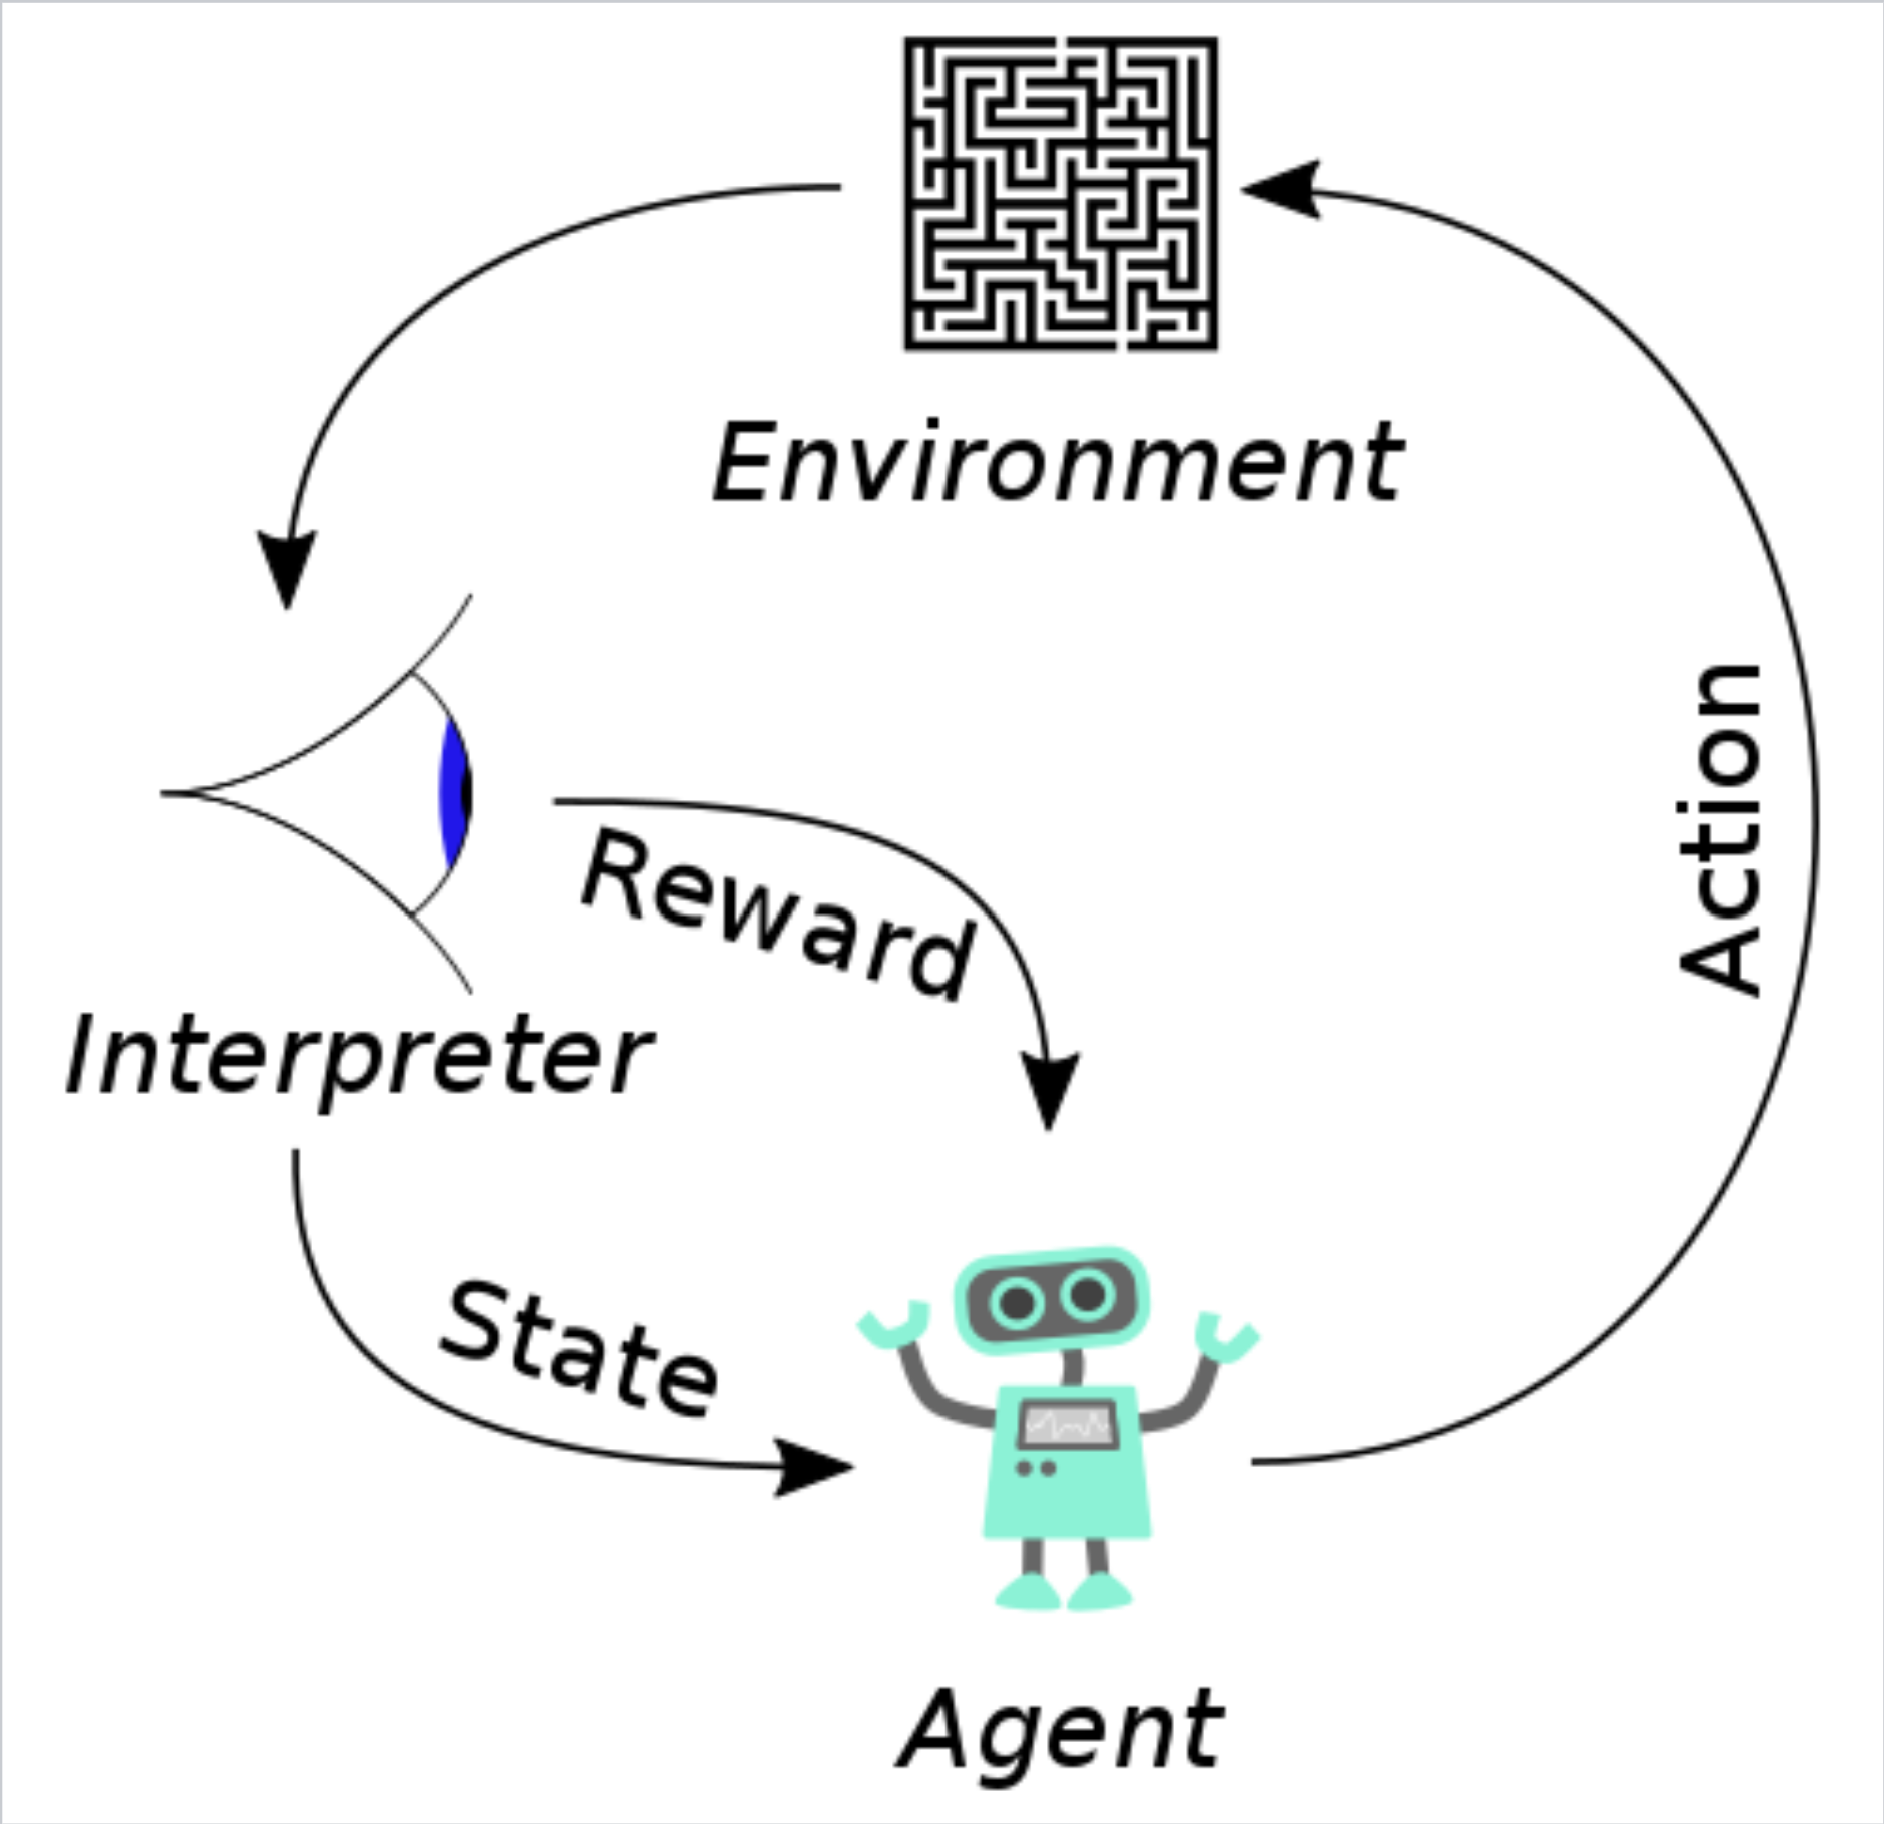
\includegraphics[width = 0.6\textwidth]{RL.png}
  \caption{强化学习工作原理}
  \label{fig_RL}
\end{figure}

\section{相关工作}
\label{related_works}
\subsection{自主导航算法}
四旋翼飞行器自主导航算法的研究已有较多成果,大体上看可以分为两类:基于优化的规划方法和基于学习的规划方法。下面将分别介绍这两类方法的研究现状。
\subsubsection{基于优化的规划方法}
同一般的无人系统一样,自主导航任务被划分为感知、规划、控制三个阶段。感知算法的任务是从传感器原始输入(如深度相机、激光雷达等)构建地图。现有的一些工作提出了从较低精度感知数据构建较高精度地图的方法\cite{heng2014autonomous}\cite{saeedi20173d}\cite{faessler2016autonomous}。而另一部分工作专注于规划无碰撞的路径而不考虑感知精度\cite{allen2016real}\cite{liu2018search}。近年来很多工作提出将这些在线建图和规划算法结合的系统,以实现在未知环境中的导航任务。例如,提出快速构建欧基里得符号距离场(Euclidean Signed Distance Fields, ESDFs)的VoxBlox\cite{oleynikova2017voxblox}、使用局部规划以提升规划效率的FASTER\cite{tordesillas2019faster}、无需构建ESDFs的规划方法EGO-Planner\cite{zhou2020ego}、考虑多无人机协同规划的EGO-swarm\cite{zhou2021ego}等。

从工程上看将导航任务分为感知、规划和控制三个子任务有不少优点:例如系统可以在不同子任务间实现并行、利用建图和规划的阶段性结果使整个系统更具可解释性等。但是三个子任务独立进行的方式忽略了不同子任务间的影响,带来了可能的累计误差,同时他们的顺序性(即下一阶段的输入为上一阶段的输出)引入了额外的延迟,为高速敏捷的飞行带来了困难\cite{falanga2019fast}。

\subsubsection{基于学习的规划方法}
总结上述工作,受限于机载计算资源和传感器精度,低延迟和高精度的感知和规划往往难以兼顾\cite{falanga2019fast}。近年来一些工作提出直接从数据中学习端到端策略而无需区分明确的感知和规划阶段。这些策略是通过模仿人类在仿真器\cite{sadeghi2016cad2rl}\cite{loquercio2021learning}或现实世界\cite{gandhi2017learning}中收集的经验训练得到的。最近的工作表明在仿真器中训练得到的敏捷的规划和控制策略可以被零成本(Zero-Shot)地迁移至部署平台\cite{kaufmann2020deep}\cite{loquercio2021learning}。但此类方法需要大量经验性的人工数据或是\cite{sadeghi2016cad2rl}或是设计复杂的专家(Expert)方法以采集足够数量的训练数据\cite{loquercio2021learning}。

\subsection{仿真器}
为加快开发速度、降低试验成本,上述两类方法均需要真实可靠的仿真器作为训练、验证的工具。尤其是随着深度强化学习技术发展,使用具有更强建模能力的基于深度学习技术的方法成为了无人系统领域的未来趋势。对于以四旋翼飞行器为代表的无人系统仿真器主要有以下三点需求:
\begin{enumerate}
  \item 仿真器能够较为真实地遵循机器人自身的物理动力学定律,并能高效地解算机器人和环境产生的交互作用。
  \item 仿真器能够集成IMU、相机、轻微系统、激光雷达等传感器。因为,这些传感器普遍应用于各项无人系统中。
  \item 仿真器能够和机器人操作系统(Robot operating system, ROS)的生态系统进行对接。ROS作为当今最完善的机器人软件系统,已经成为了标准的开发机器人应用的主流工具。
\end{enumerate}
国内外已有的针对无人机的仿真器主要有以下三个:

微软(Microsoft)公司于2017年提出了AirSim无人机驾驶自动控制仿真平台\cite{airsim2017},可实现基于虚幻引擎的无人机驾驶自动控制仿真功能。同时具备普通相机,立体相机,激光雷达,全球定位系统(GPS),IMU,磁力计等传感器。

苏黎世联邦理工学院提出了Flightmare四旋翼飞行器仿真平台\cite{flightmare},由两个主要组件组成:基于Unity的渲染引擎和可用于动力学模拟的物理引擎。且两个组件完全解耦、可以独立运行。该仿真器支持ROS环境,平台上集成了丰富的传感器,包括普通相机,立体相机,IMU等。

多伦多大学提出了Gym-pybullet-drones四旋翼飞行器仿真平台\cite{pybullet},同样集成了普通相机,立体相机,IMU等的传感器,可实现无人机集群的模拟,同时支持与ROS2系统通信。

三者采用了不同的物理引擎和和界面渲染,都支持ROS、视觉传感器模块,且考虑了空气动力学因素。但是三者的仿真运行速度较慢,仿真每秒状态数(Frame per second, FPS)$<100$。难以满足强化学习等需要大量仿真数据算法的需求。

\subsection{部署平台}
四旋翼飞行器部署平台具有结构相对简单、成本相对较低的优点。常见的科研用四旋翼无人机平台,如Crazyfile\cite{crazyfly},具有结构简单、结实耐用的优点,但并不搭载感知和计算单元,依靠上位机完成整个任务流程。此类平台常用于做科研算法快速验证而无法实际部署应用,如图\ref{fig_crazyfile}所示。最近一些无人系统工作选择将其仿真平台硬件开源\cite{zhou2020ego},但其部署平台和部署系统接口高度定制化,难以二次开发,如图\ref{fig_egofly}。一些国内外公司专门研发了科研用无人机\cite{amove},但其商品化程度高,飞行性能低,不便有效的改装和定制,如图\ref{fig_amove}。
\begin{figure}
  \centering
    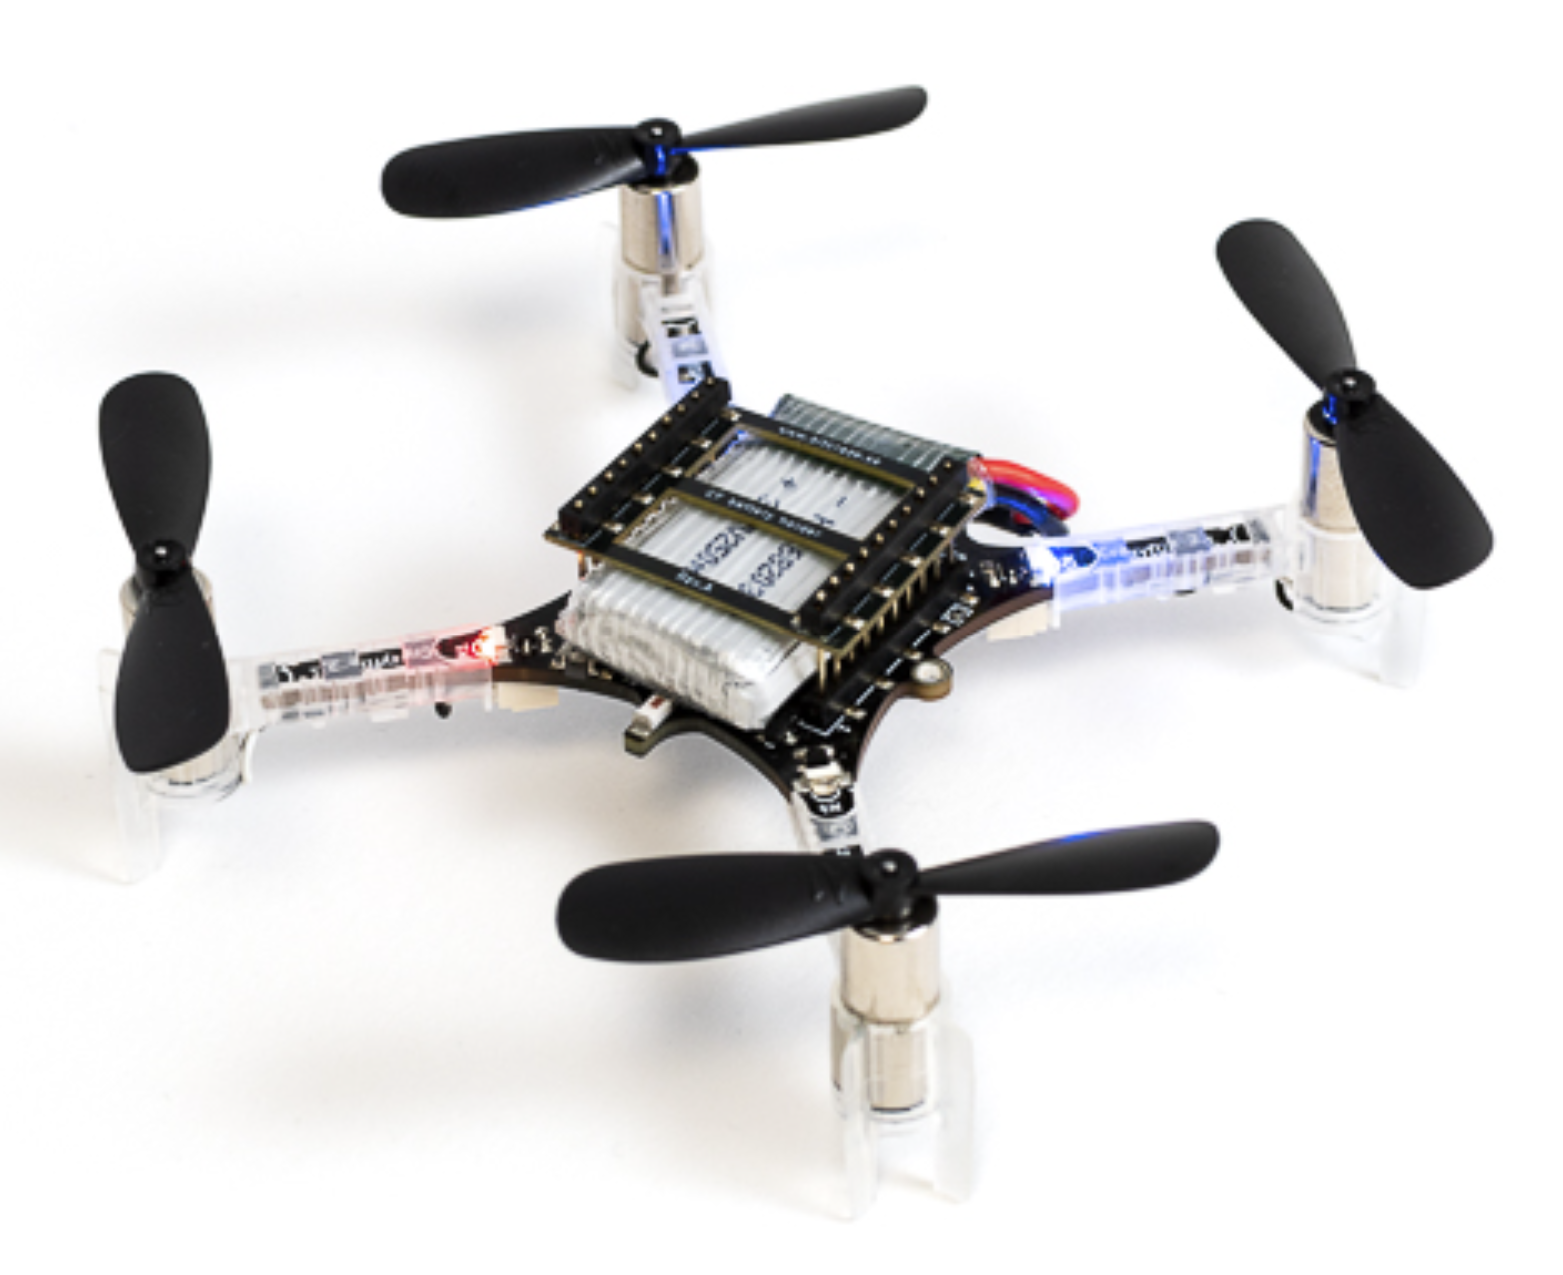
\includegraphics[width = 0.6\textwidth]{crazyfile.png}
    \caption{Crazyfile无人机}
    \label{fig_crazyfile}
\end{figure}
\begin{figure}
  \centering
    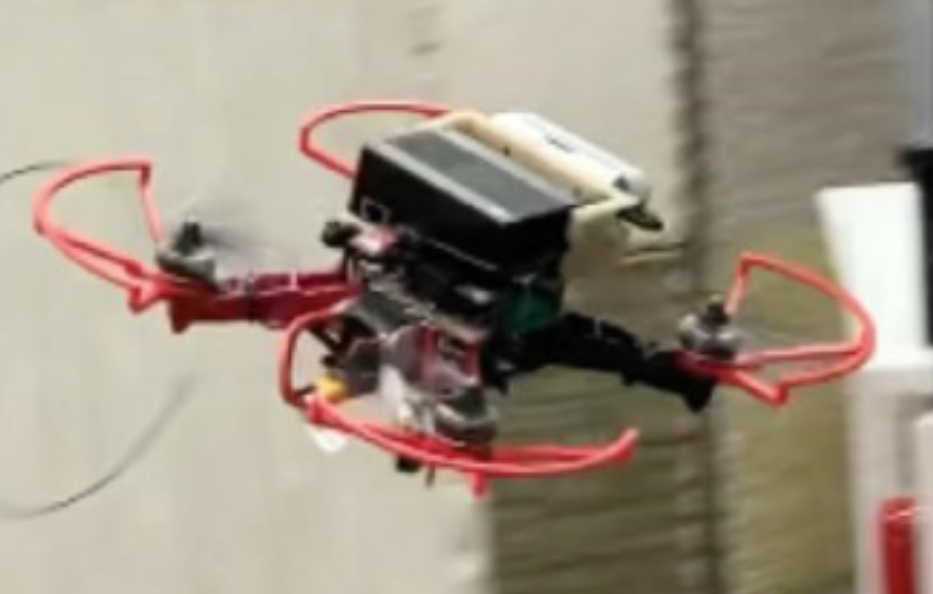
\includegraphics[width = 0.6\textwidth]{egofly.png}
    \caption{ego-planner项目硬件开源的无人机}
    \label{fig_egofly}
\end{figure}
\begin{figure}
  \centering
    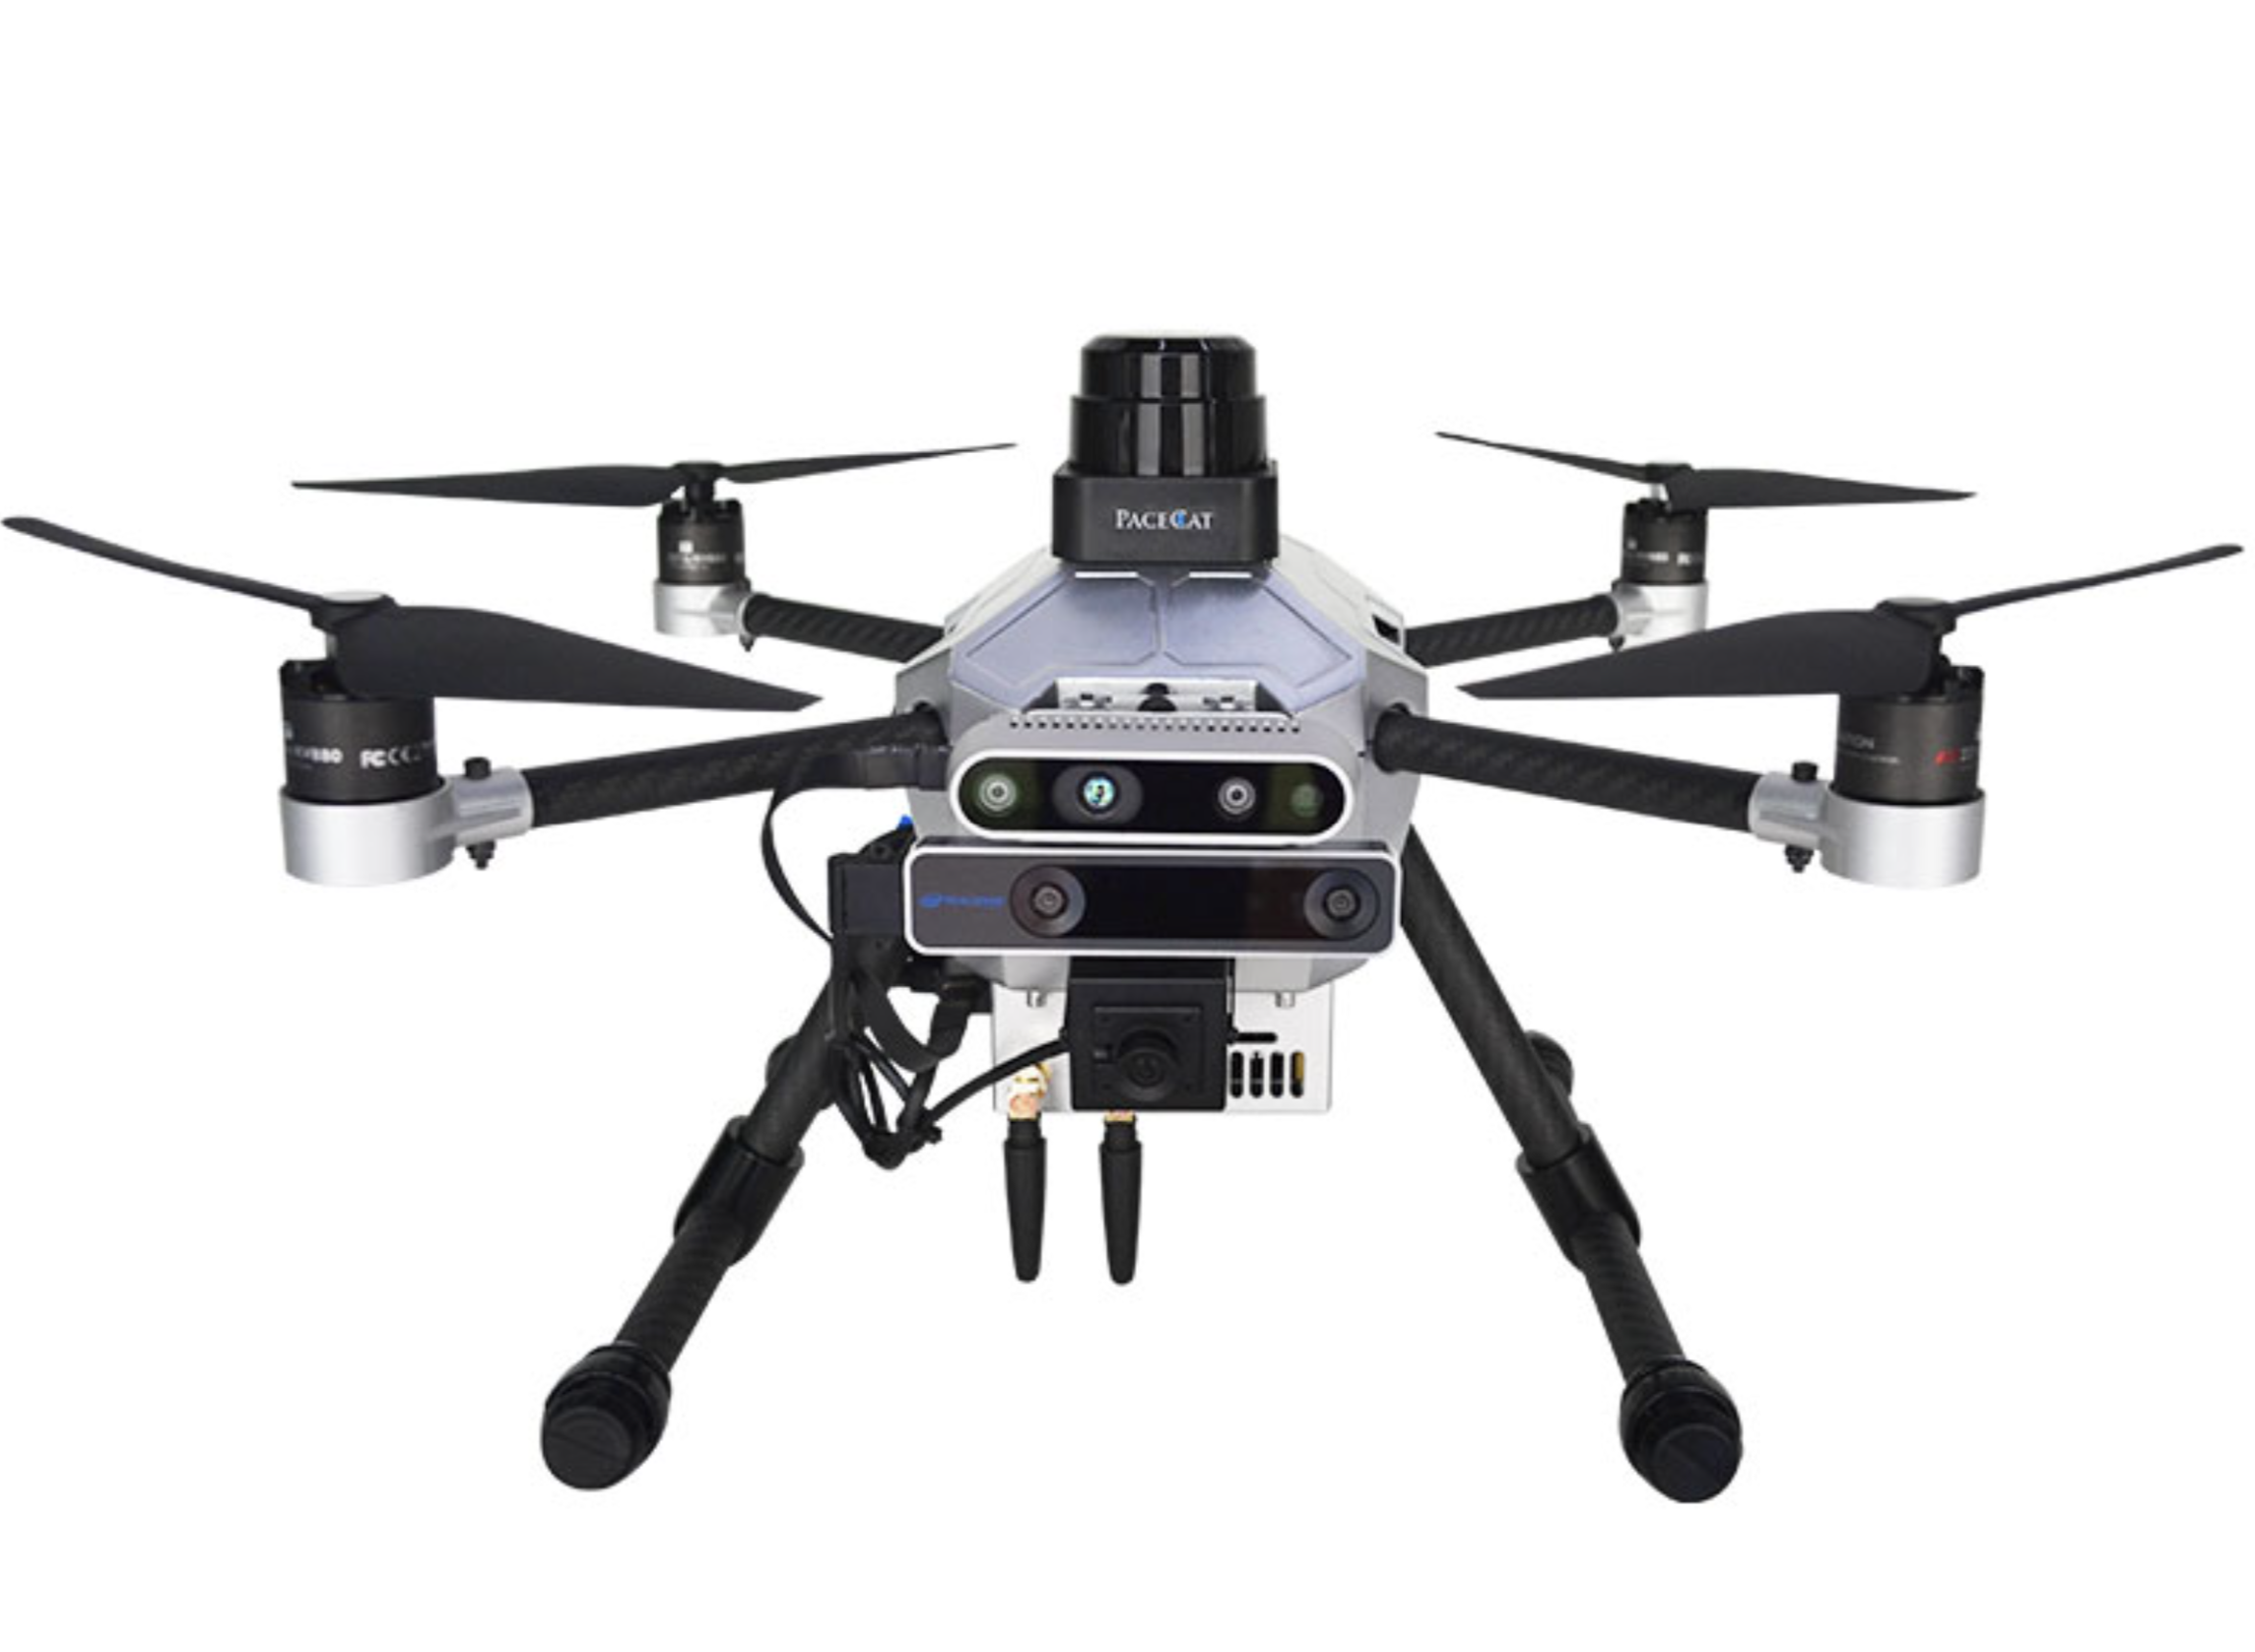
\includegraphics[width = 0.6\textwidth]{amove.png}
    \caption{市售科研用无人机}
    \label{fig_amove}
\end{figure}

\section{研究目的}
\label{target}
本研究面向面向以四旋翼飞行器为代表的无人机的自主导航任务,设计一种高效的自主导航算法。自主导航任务的定义如图\ref{fig_task_define}所示。自主导航指的是一类在没有环境地图,没有外部定位、通信和操纵指令情况下自主通过未知区域并到达目标点的任务。
\begin{figure}
  \centering
  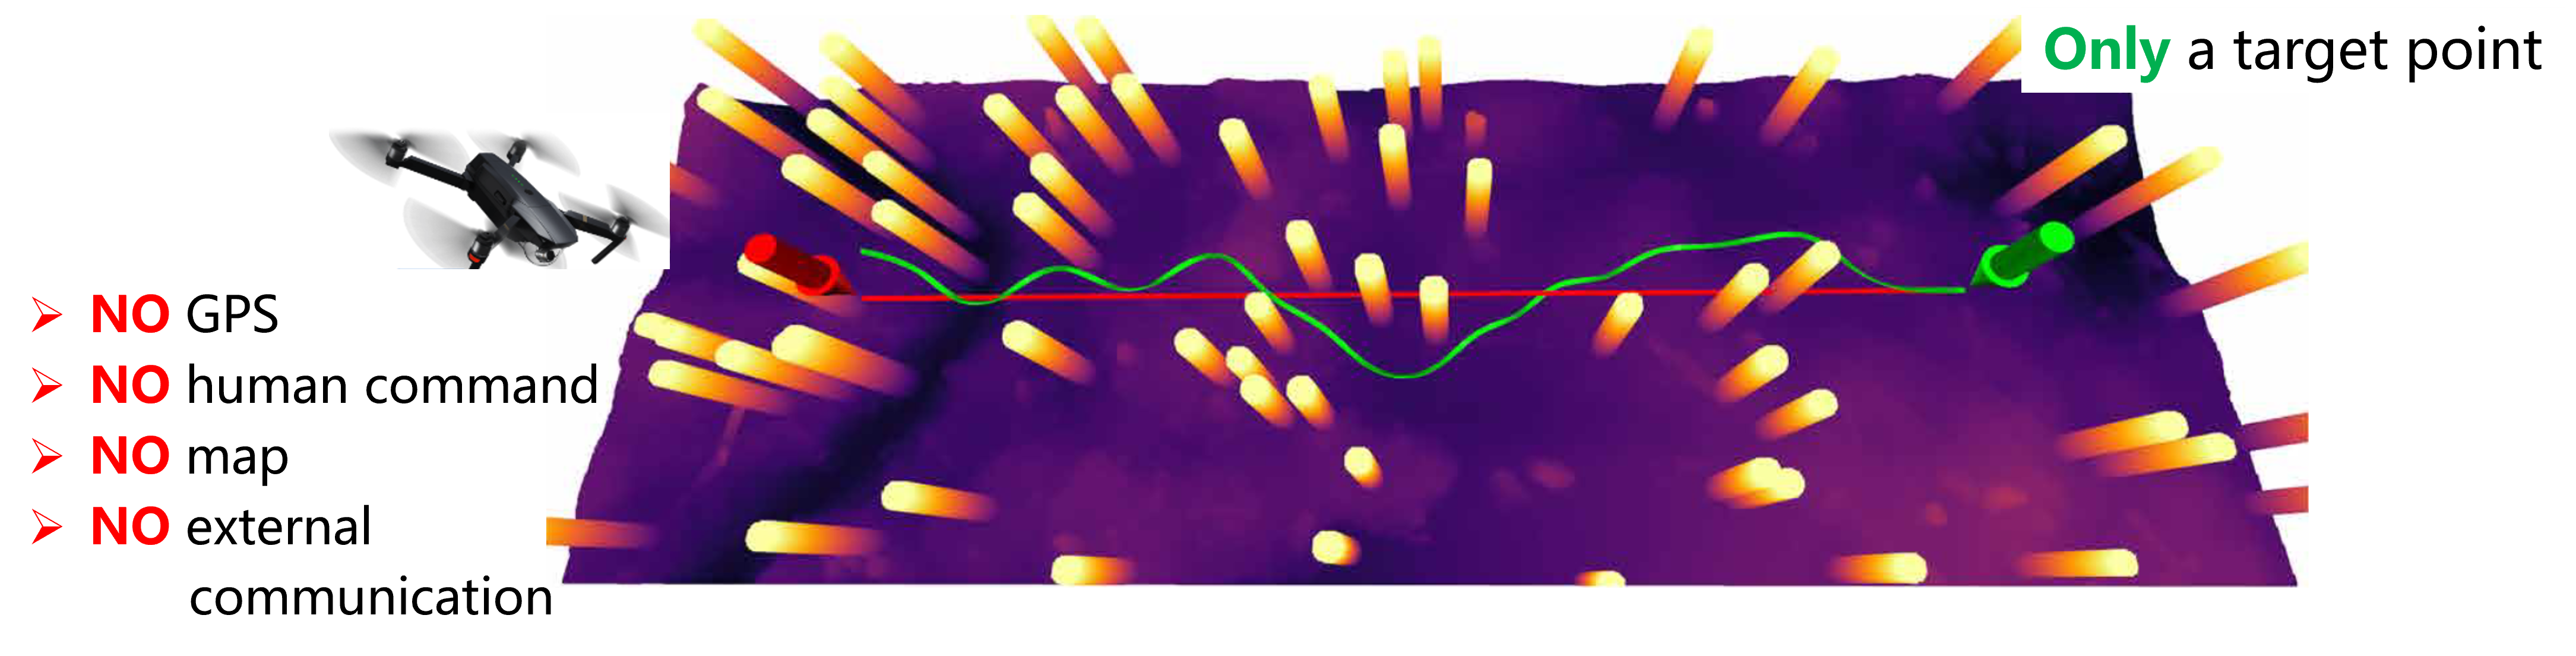
\includegraphics[width = 0.97\textwidth]{task.png}
  \caption{自主导航任务示意图}
  \label{fig_task_define}
\end{figure}

总结\ref{background}和\ref{related_works}节中提到的需求和研究现状,以四旋翼无人机完成自主导航任务存在以下三个挑战:
\begin{enumerate}
  \item 常用的无人机仿真器存在拟真度和仿真速度的矛盾。根据调研和实验,拟真度较高的仿真器虽然可以实现零成本部署,但采集数据速度慢,采集一条轨迹数据需要约90s时间\cite{loquercio2021learning}。而采集数据速度较快的仿真器往往难以直接部署\cite{zhu2022viola}。
  \item 现存的无人机自主导航算法难以满足需求。基于感知算法的使用优化方法的规划器规划速度慢,算力需求高\cite{ren2022bubble}。而基于人类专家数据的深度学习方法虽然很好的解决了规划速度的问题,但需要较大量的人类专家数据\cite{loquercio2021learning},需要大量经验性的设定。
  \item 目前尚没有一种功能齐全、接口丰富、运行稳定的成熟的无人机平台供自主导航任务使用。
\end{enumerate}

本研究聚焦无人机在无外部定位、通信、操纵情况下的自主导航任务。对应于上述三个挑战,主要研究内容有三:
\begin{enumerate}
  \item 基于现有仿真器,通过增加并行度等方法提高仿真器采集数据的速度以满足强化学习算法对大量数据的需求。
  \item 设计一种基于强化学习的无人机自主导航算法,并设计配套的训练方法。在利用强化学习算法解决算法运行速度慢、需要大量专家数据这两个问题的同时也尽可能规避其自身存在的数据效率低、收敛慢等问题。
  \item 设计并搭建具有自主定位、自主计算的四旋翼无人机并设计一套部署系统。该部署系统应集成多种传感器和多种控制器供选择,并预留完善的算法接口。最后在该算法平台上验证自主导航算法的实际飞行效果。
\end{enumerate}
本研究的研究框架如图\ref{fig_outline}所示。
\begin{figure}
  \centering
  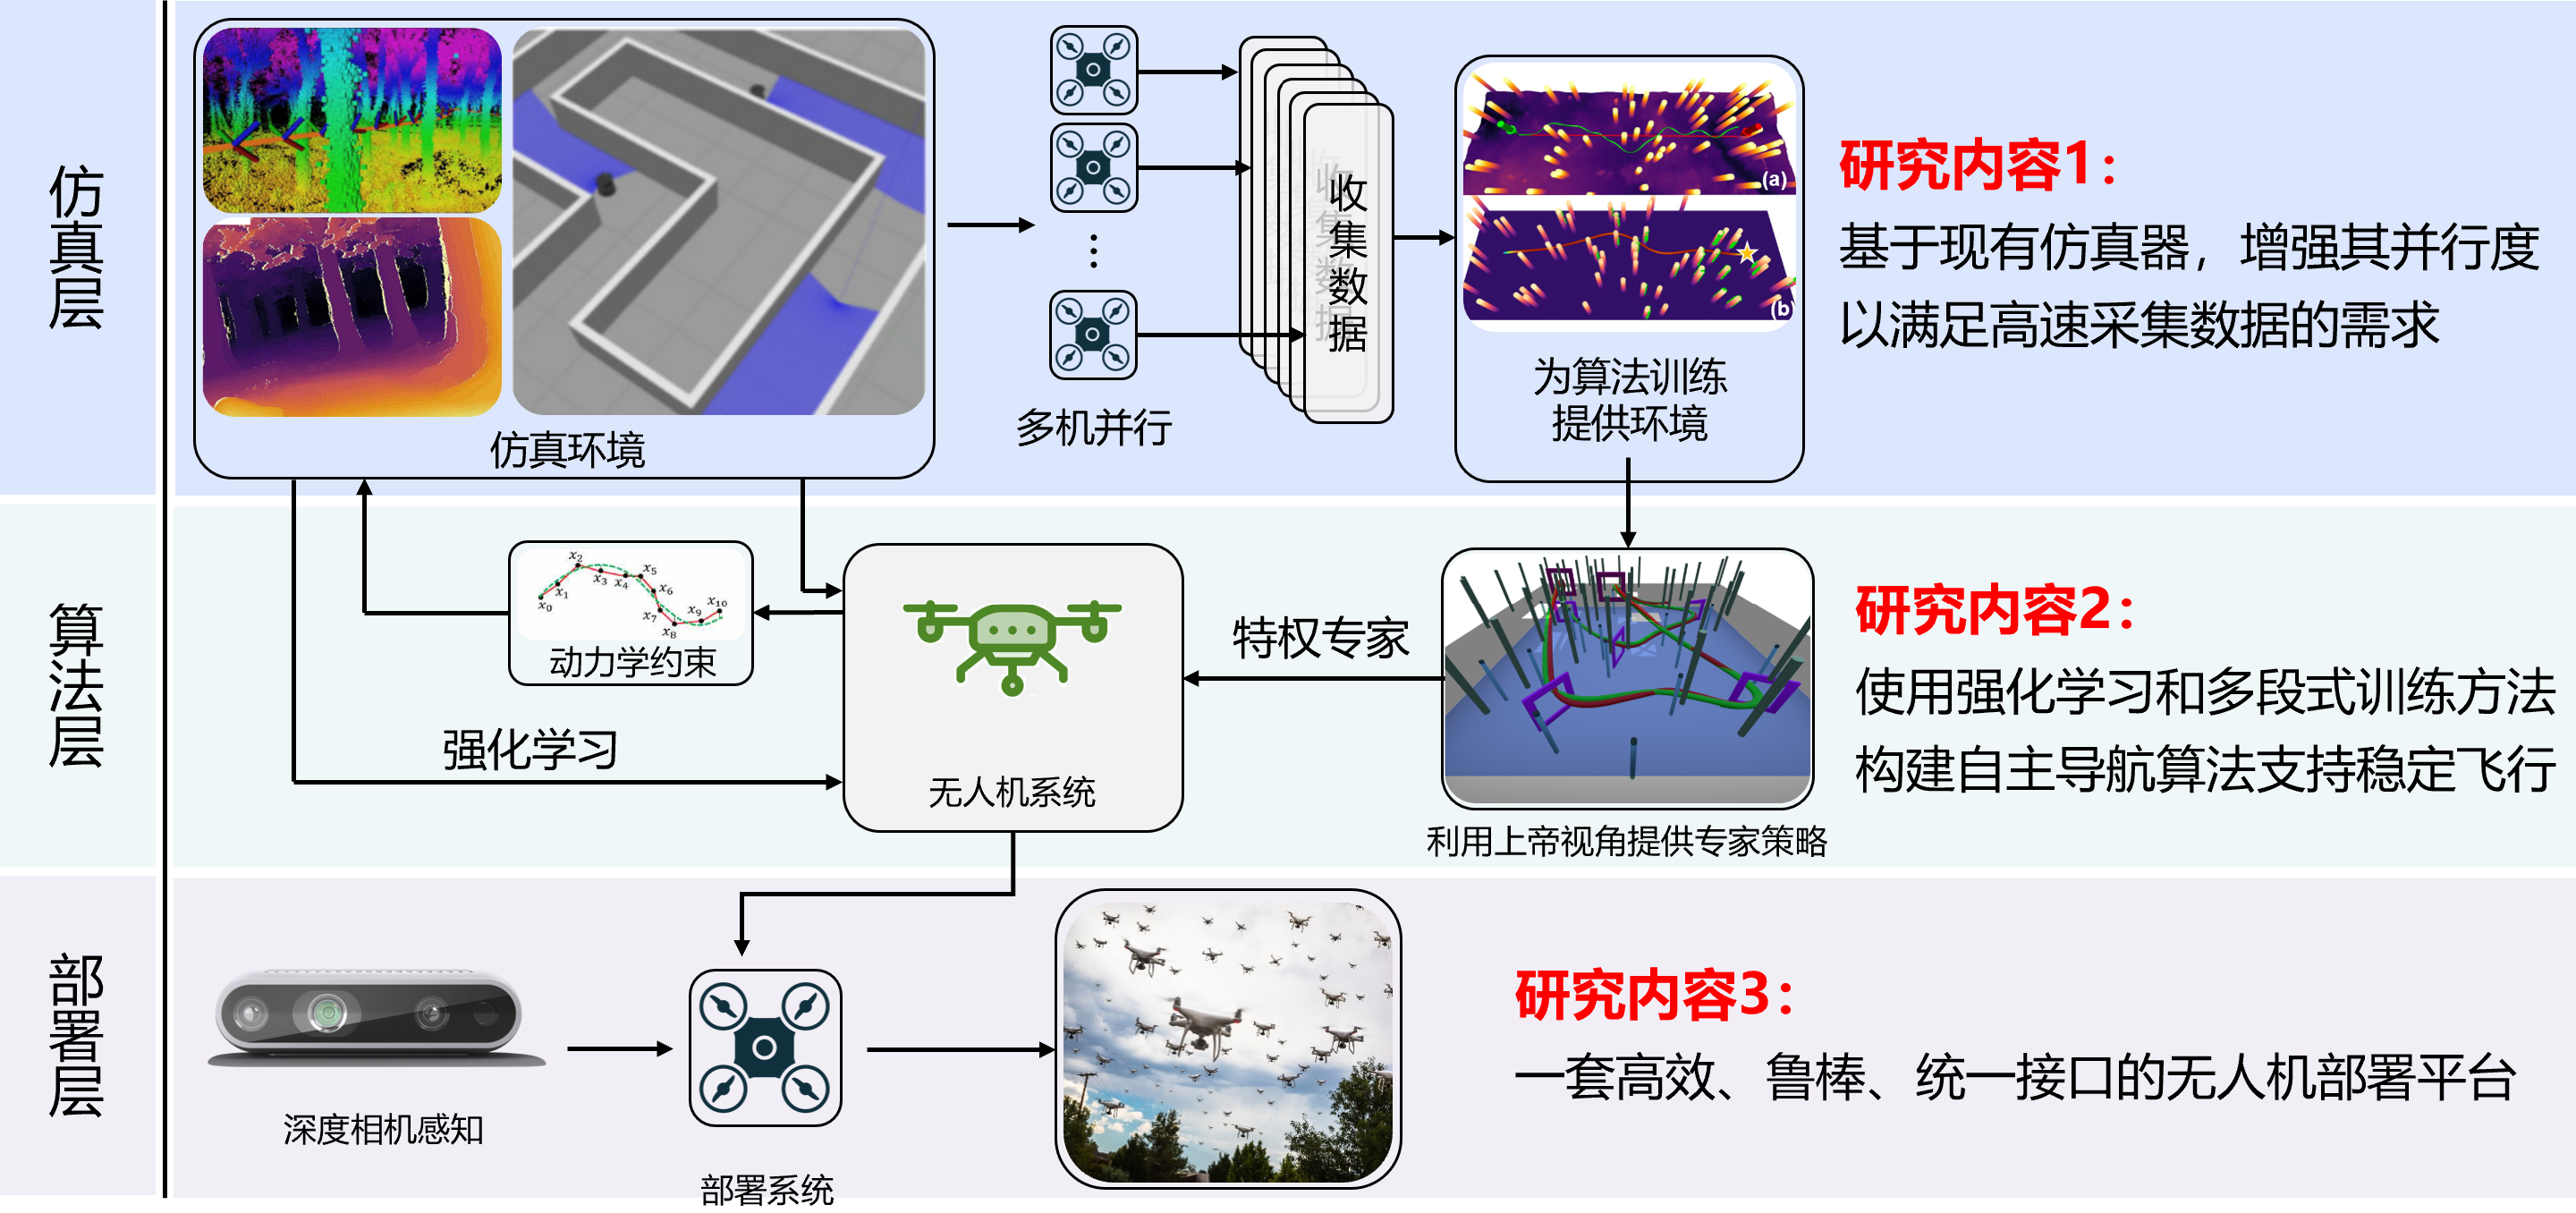
\includegraphics[width = 1\textwidth]{outline.png}
  \caption{研究框架示意图}
  \label{fig_outline}
\end{figure}

本研究是一个系统性研究,其中强化学习算法设计部分为主要的创新点。仿真器和部署平台包含则较多工程技巧,工作量较大,但这是完成算法训练和算法验证必不可少的环节。同时本项目所设计的仿真器和部署平台将作为课题组后续相关研究重要的基础设施。

\section{各章节概述}
\label{outline}
本研究报告共分为六章,本章主要介绍了本研究的背景、现存挑战,从应用和学术研究的角度阐述了本研究的必要性和挑战性。第二章至第四章分别介绍了仿真器的改进工作、强化学习算法和部署平台的结构设计,并简要介绍这些设计对总体飞行性能的影响。第五章介绍了本研究的实验结果,包括仿真平台参数的设置,算法调试的结果和实机部署的结果。第六章对本研究做一个整体总结并提出该项目未来可继续改进的方向。


% \section{引言的写法}

% 一篇学位论文的引言大致包含如下几个部分:
% 1、问题的提出;
% 2、选题背 景及意义;
% 3、文献综述;
% 4、研究方法;
% 5、论文结构安排。
% \begin{itemize}
%   \item 问题的提出:要清晰地阐述所要研究的问题“是什么”。
%     \footnote{选题时切记要有“问题意识”,不要选不是问题的问题来研究。}
%   \item 选题背景及意义:论述清楚为什么选择这个题目来研究,即阐述该研究对学科发展的贡献、对国计民生的理论与现实意义等。
%   \item 文献综述:对本研究主题范围内的文献进行详尽的综合述评,“述”的同时一定要有“评”,指出现有研究状态,仍存在哪些尚待解决的问题,讲出自己的研究有哪些探索性内容。
%   \item 研究方法:讲清论文所使用的学术研究方法。
%   \item 论文结构安排:介绍本论文的写作结构安排。
% \end{itemize}



% \section{正文的写法}

% 本部分是论文作者的研究内容,不能将他人研究成果不加区分地掺和进来。
% 已经在引言的文献综述部分讲过的内容,这里不需要再重复。
% 各章之间要存在有机联系,符合逻辑顺序。



% \section{结论的写法}

% 结论是对论文主要研究结果、论点的提炼与概括,应精炼、准确、完整,使读者看后能全面了解论文的意义、目的和工作内容。
% 结论是最终的、总体的结论,不是正文各章小结的简单重复。
% 结论应包括论文的核心观点,主要阐述作者的创造性工作及所取得的研究成果在本领域中的地位、作用和意义,交代研究工作的局限,提出未来工作的意见或建议。
% 同时,要严格区分自己取得的成果与指导教师及他人的学术成果。

% 在评价自己的研究工作成果时,要实事求是,除非有足够的证据表明自己的研究是“首次”、“领先”、“填补空白”的,否则应避免使用这些或类似词语。

% !TeX root = ../thuthesis-example.tex

\chapter{仿真器改进}
本章主要介绍高并行度仿真器的设计和开发。本研究以苏黎世联邦理工大学开发的FLightmare\cite{flightmare}仿真器为基础,增加了并行设计以加快仿真速度。由于该仿真器使用Gazebo作为物理引擎,Unity作为渲染引擎,因此该仿真器仿真度较高。本章将介绍Flightmare仿真器的基本情况和本研究所做的改进。

\section{仿真器基本情况}
FLightmare仿真器\cite{flightmare}是苏黎世联邦理工大学开发的一款四旋翼飞行器仿真平台。使用Gazebo作为物理引擎并使用Unity作为渲染引擎,两个模块可分开运行。仿真器的原始结构如图\ref{fig_simulator_origin}所示。
\begin{figure}
  \centering
  
\includegraphics[width = 0.75\textwidth]{simulator_origin.png}
  \caption{FLightmare仿真器结构图}
  \label{fig_simulator_origin}
\end{figure}

\subsection{Gazebo简介}
Gazebo是加州大学提出的机器人仿真平台(平台界面如图\ref{fig_gazebo}所示),可实现对于复杂的室内外环境精确的模拟一个或多个机器人的运动。Gazebo的多体动力学模拟精确,但图形渲染能力羸弱,只能够使用CPU资源仿真简单的传感器模块,随着场景变得复杂,仿真运行速度会急剧降低。
\begin{figure}
  \centering
  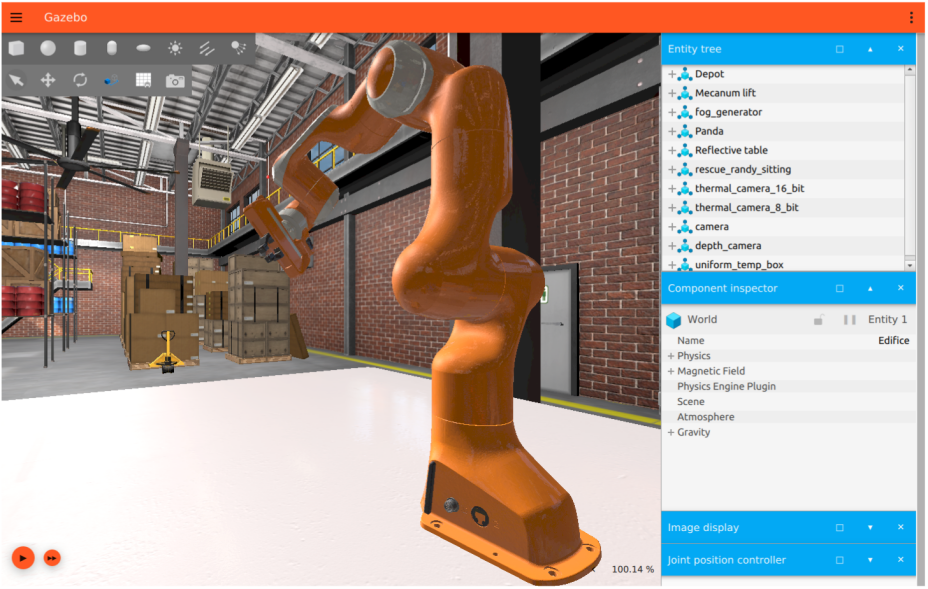
\includegraphics[width = 0.7\textwidth]{gazebo.png}
  \caption{Gazebo物理引擎界面示意图}
  \label{fig_gazebo}
\end{figure}
Gazebo对于ROS生态支持效果较好。因此多出现在使用ROS的仿真平台中。

\subsection{Unity简介}
Unity是一款跨平台的二维和三维游戏引擎\cite{unity},拥有强大的建模和渲染能力。在本仿真器中,Unity主要负责构建场景,并渲染相机、激光雷达等传感器的结果。图\ref{fig_pointcloud}是Unity引擎渲染出树林场景的点云(Pointcloud)数据,图\ref{fig_camera}是同场景对应的图像和深度图像渲染效果。
\begin{figure}
  \centering
  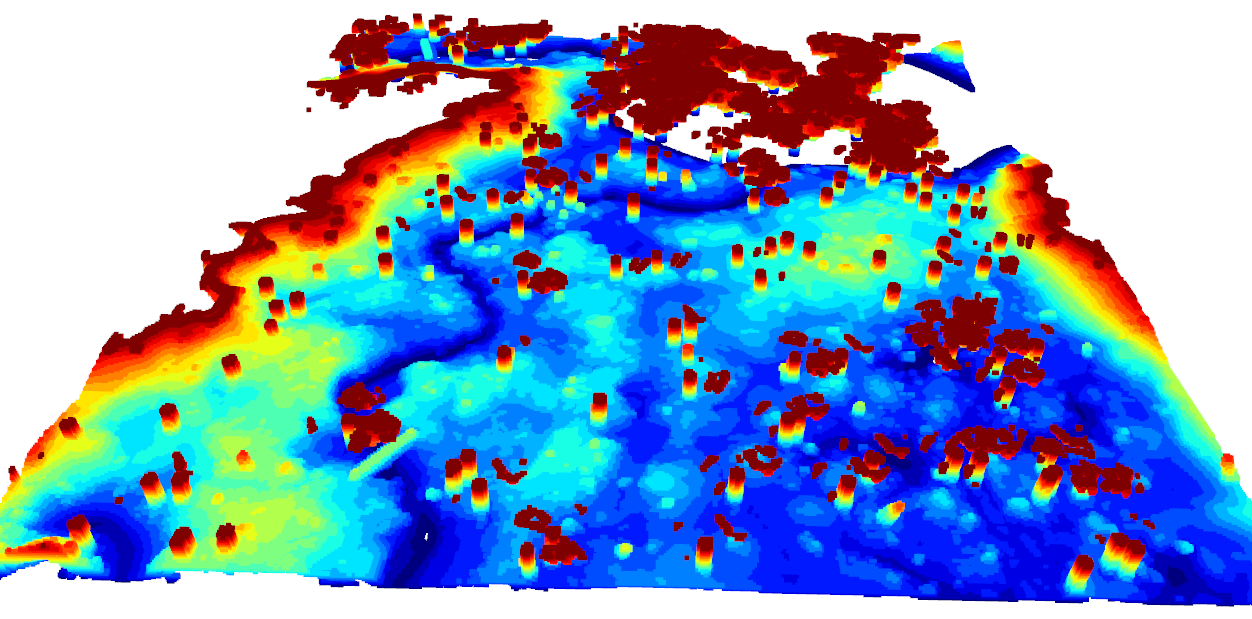
\includegraphics[width = 0.9\textwidth]{pointcloud.png}
  \caption{Unity渲染点云效果示意图}
  \label{fig_pointcloud}
\end{figure}
\begin{figure}
  \centering  
  \subcaptionbox{图像渲染}
    {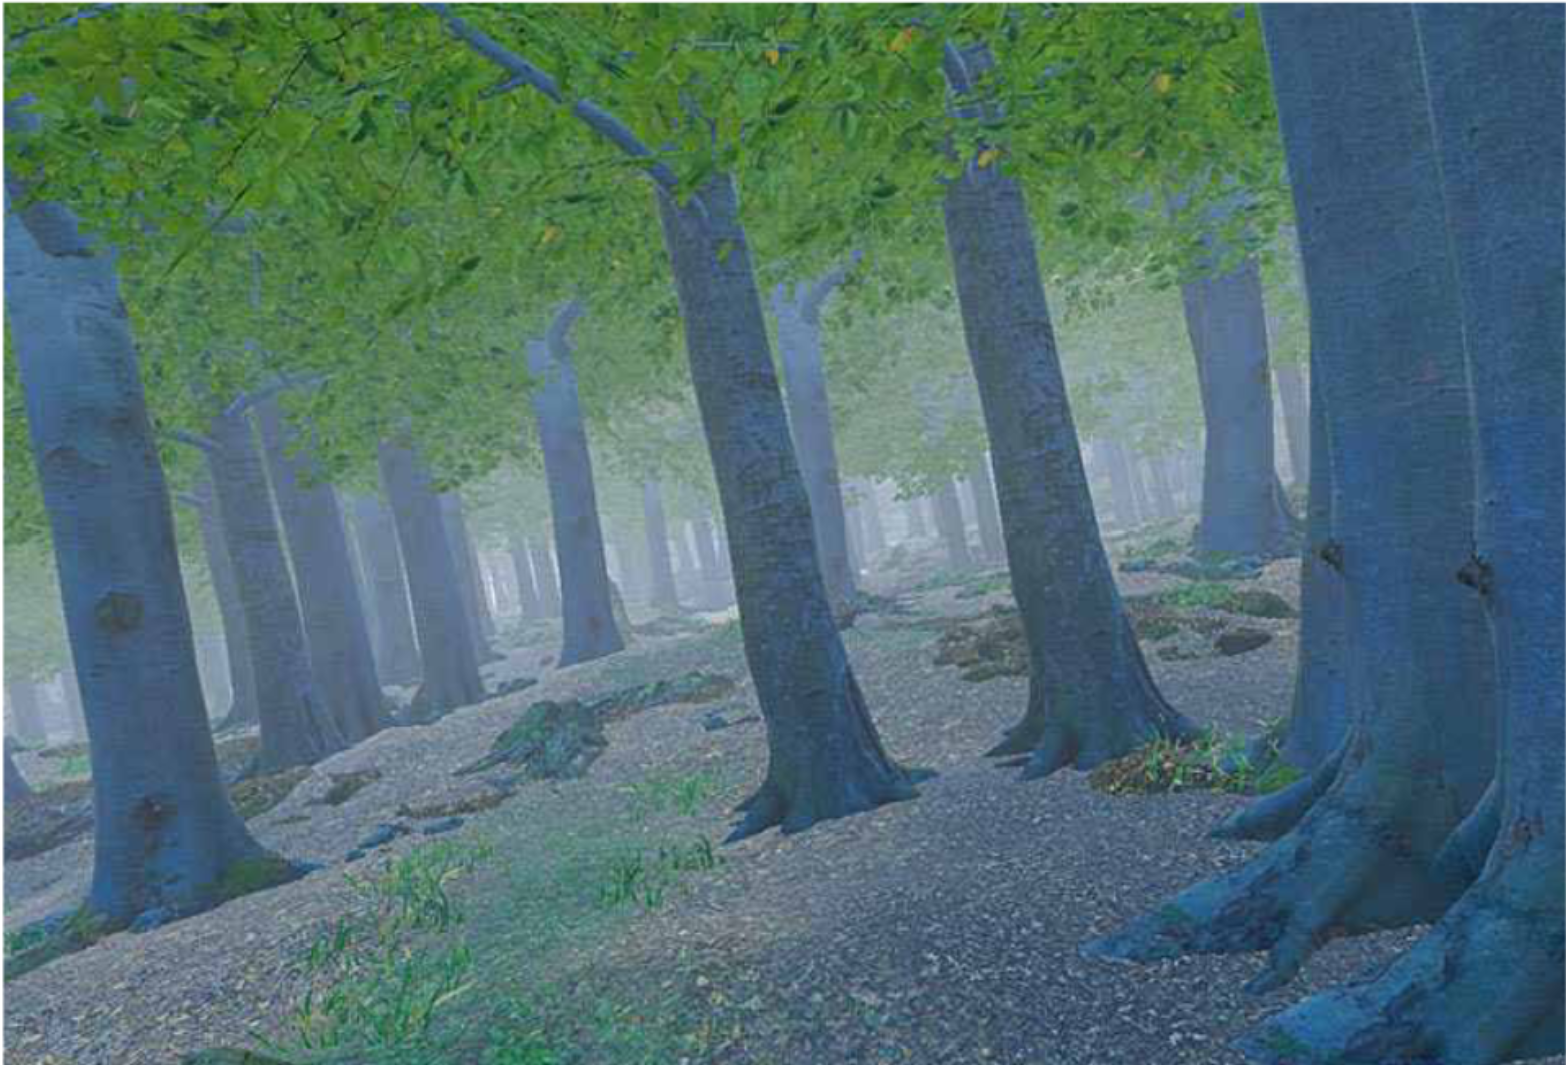
\includegraphics[width=0.45\linewidth]{rgbcamera.png}}
  \subcaptionbox{深度图渲染}
    {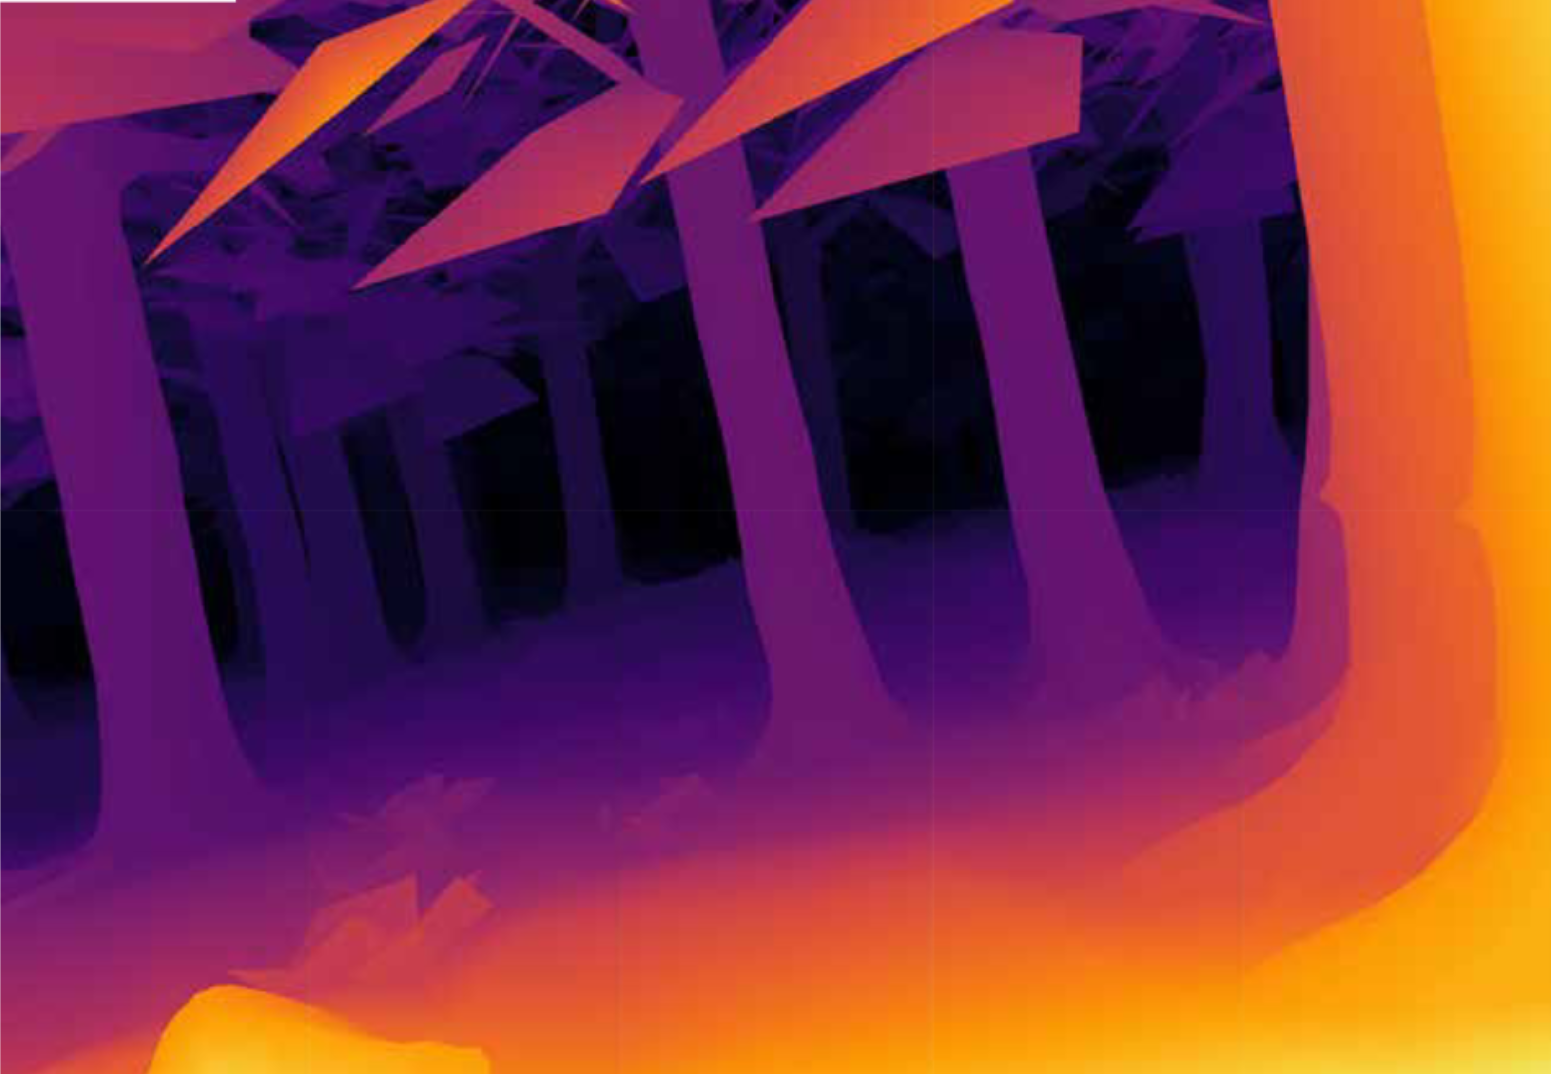
\includegraphics[width=0.45\linewidth]{depcamera.png}}
  \caption{Unity渲染效果示意图}
  \label{fig_camera}
\end{figure}

\section{仿真器加速改进}
\subsection{仿真器加速设计}
本研究利用ROS和Unity的特性通过多线程并行实现了仿真器的加速,具体工作有如下三点:
\begin{enumerate}
  \item 多线程并行Unity,并在Gazebo内并行起飞多架无人机
  \item 使用统一的桥接(Bridge)节点负责Unity和Gazebo的通信
  \item 并行控制器节点为每台飞机提供独立控制
\end{enumerate}

除此之外,受限于单台计算机计算资源,利用ROS的分布式特性还可以在局域网内搭建分布式仿真器结构,进一步加快仿真速度。改造完成的仿真器结构如图\ref{fig_simulator_multi}所示。

在Intel i9 + Nvidia RTX 4090配置的测试平台上实验,改进后的仿真器在每台机器上最多并行2台无人机,通过局域网至多连接3台机器,实现2*3倍并行,训练强化学习算法的速度可提升6倍。
\begin{figure}
  \centering
  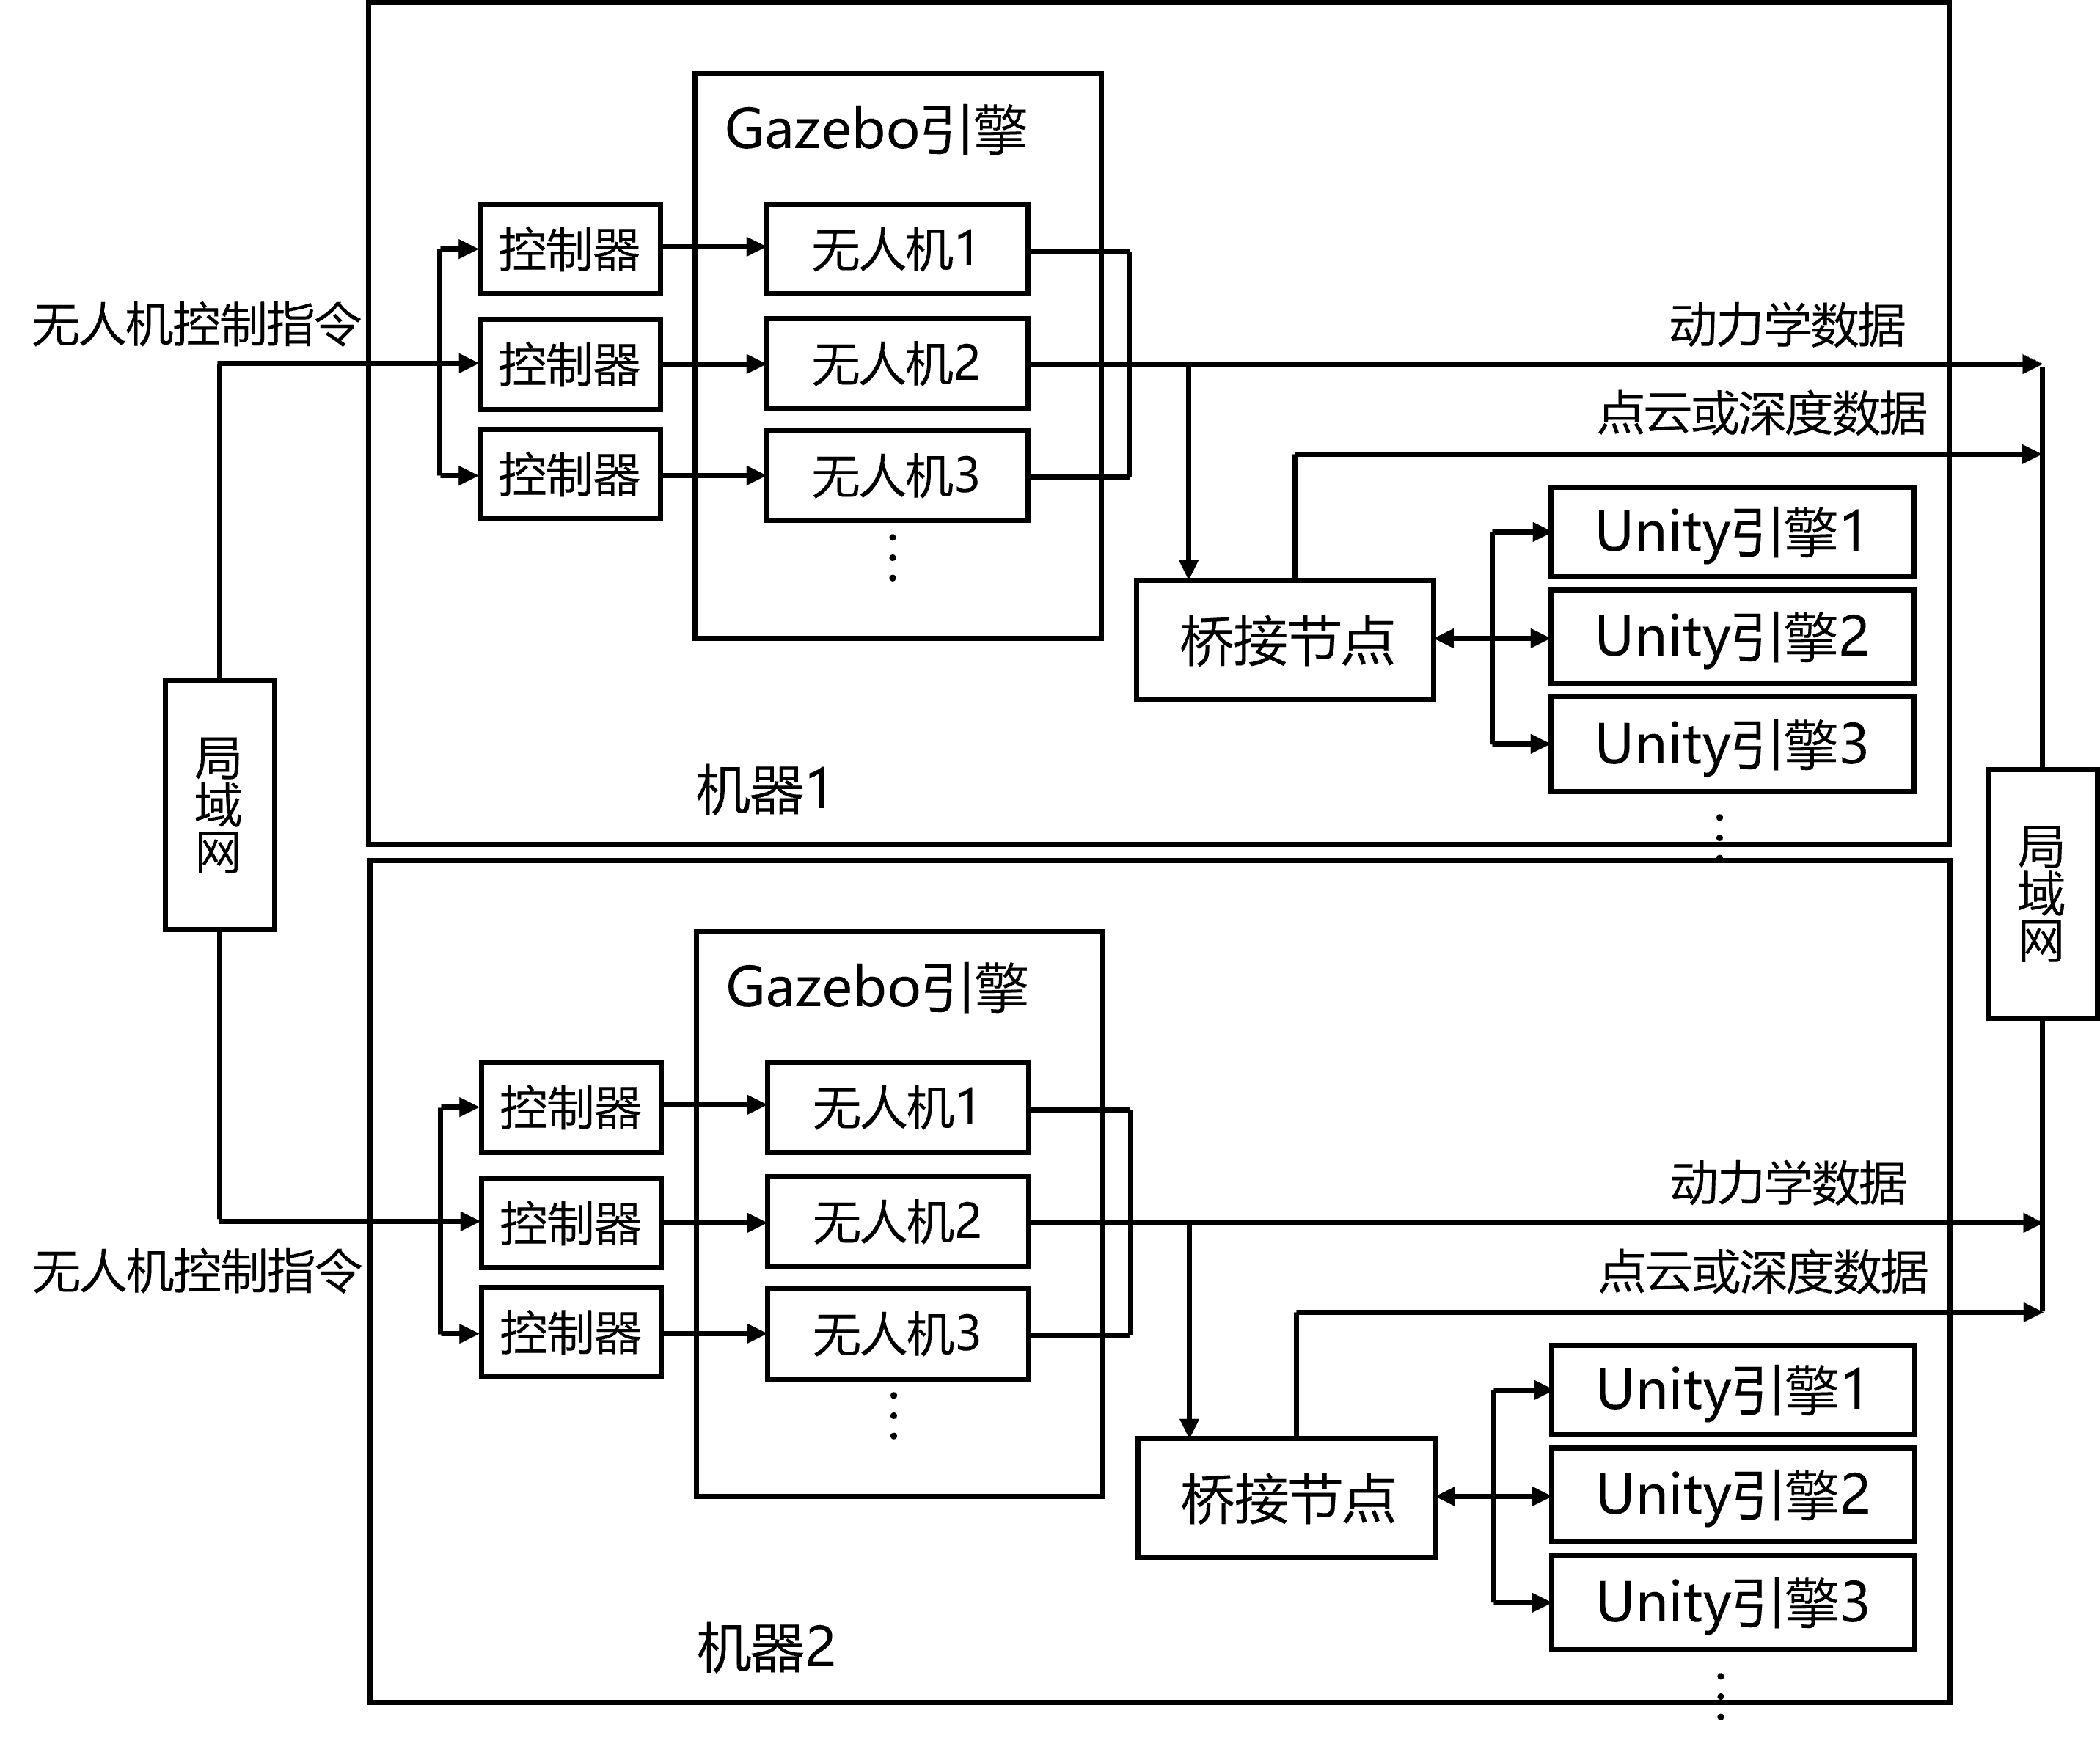
\includegraphics[width = 1\textwidth]{simulator_multi.png}
  \caption{改进后仿真器结构图}
  \label{fig_simulator_multi}
\end{figure}

\section{本章小结}

本章介绍了本研究所使用基础仿真器的基本情况。并介绍了对基础仿真器进行改动的设计。经过并行化设计仿真器的仿真速度得到了大幅提升,为后续算法研究和训练提供了保障。经过测试,改进后仿真器收集算法收敛所需的数据花费的时间约为48$\sim$72小时。


% \section{插图}

% 图片通常在 \env{figure} 环境中使用 \cs{includegraphics} 插入,如图~\ref{fig:example} 的源代码。
% 建议矢量图片使用 PDF 格式,比如数据可视化的绘图;
% 照片应使用 JPG 格式;
% 其他的栅格图应使用无损的 PNG 格式。
% 注意,LaTeX 不支持 TIFF 格式;EPS 格式已经过时。

% \begin{figure}
%   \centering
%   
\includegraphics[width=0.5\linewidth]{example-image-a.pdf}
%   \caption*{国外的期刊习惯将图表的标题和说明文字写成一段,需要改写为标题只含图表的名称,其他说明文字以注释方式写在图表下方,或者写在正文中。}
%   \caption{示例图片标题}
%   \label{fig:example}
% \end{figure}

% 若图或表中有附注,采用英文小写字母顺序编号,附注写在图或表的下方。
% 国外的期刊习惯将图表的标题和说明文字写成一段,需要改写为标题只含图表的名称,其他说明文字以注释方式写在图表下方,或者写在正文中。

% 如果一个图由两个或两个以上分图组成时,各分图分别以 (a)、(b)、(c)...... 作为图序,并须有分图题。
% 推荐使用 \pkg{subcaption} 宏包来处理, 比如图~\ref{fig:subfig-a} 和图~\ref{fig:subfig-b}。

% \begin{figure}
%   \centering
%   \subcaptionbox{分图 A\label{fig:subfig-a}}
%     {
\includegraphics[width=0.35\linewidth]{example-image-a.pdf}}
%   \subcaptionbox{分图 B\label{fig:subfig-b}}
%     {
\includegraphics[width=0.35\linewidth]{example-image-b.pdf}}
%   \caption{多个分图的示例}
%   \label{fig:multi-image}
% \end{figure}



% \section{表格}

% 表应具有自明性。为使表格简洁易读,尽可能采用三线表,如表~\ref{tab:three-line}。
% 三条线可以使用 \pkg{booktabs} 宏包提供的命令生成。

% \begin{table}
%   \centering
%   \caption{三线表示例}
%   \begin{tabular}{ll}
%     \toprule
%     文件名          & 描述                         \\
%     \midrule
%     thuthesis.dtx   & 模板的源文件,包括文档和注释 \\
%     thuthesis.cls   & 模板文件                     \\
%     thuthesis-*.bst & BibTeX 参考文献表样式文件    \\
%     \bottomrule
%   \end{tabular}
%   \label{tab:three-line}
% \end{table}

% 表格如果有附注,尤其是需要在表格中进行标注时,可以使用 \pkg{threeparttable} 宏包。
% 研究生要求使用英文小写字母 a、b、c……顺序编号,本科生使用圈码 ①、②、③……编号。

% \begin{table}
%   \centering
%   \begin{threeparttable}[c]
%     \caption{带附注的表格示例}
%     \label{tab:three-part-table}
%     \begin{tabular}{ll}
%       \toprule
%       文件名                 & 描述                         \\
%       \midrule
%       thuthesis.dtx\tnote{a} & 模板的源文件,包括文档和注释 \\
%       thuthesis.cls\tnote{b} & 模板文件                     \\
%       thuthesis-*.bst        & BibTeX 参考文献表样式文件    \\
%       \bottomrule
%     \end{tabular}
%     \begin{tablenotes}
%       \item [a] 可以通过 xelatex 编译生成模板的使用说明文档;
%         使用 xetex 编译 \file{thuthesis.ins} 时则会从 \file{.dtx} 中去除掉文档和注释,得到精简的 \file{.cls} 文件。
%       \item [b] 更新模板时,一定要记得编译生成 \file{.cls} 文件,否则编译论文时载入的依然是旧版的模板。
%     \end{tablenotes}
%   \end{threeparttable}
% \end{table}

% 如某个表需要转页接排,可以使用 \pkg{longtable} 宏包,需要在随后的各页上重复表的编号。
% 编号后跟表题(可省略)和“(续)”,置于表上方。续表均应重复表头。

% \begin{longtable}{cccc}
%     \caption{跨页长表格的表题}
%     \label{tab:longtable} \\
%     \toprule
%     表头 1 & 表头 2 & 表头 3 & 表头 4 \\
%     \midrule
%   \endfirsthead
%     \caption*{续表~\thetable\quad 跨页长表格的表题} \\
%     \toprule
%     表头 1 & 表头 2 & 表头 3 & 表头 4 \\
%     \midrule
%   \endhead
%     \bottomrule
%   \endfoot
%   Row 1  & & & \\
%   Row 2  & & & \\
%   Row 3  & & & \\
%   Row 4  & & & \\
%   Row 5  & & & \\
%   Row 6  & & & \\
%   Row 7  & & & \\
%   Row 8  & & & \\
%   Row 9  & & & \\
%   Row 10 & & & \\
% \end{longtable}



% \section{算法}

% 算法环境可以使用 \pkg{algorithms} 或者 \pkg{algorithm2e} 宏包。

% \renewcommand{\algorithmicrequire}{\textbf{输入:}\unskip}
% \renewcommand{\algorithmicensure}{\textbf{输出:}\unskip}

% \begin{algorithm}
%   \caption{Calculate $y = x^n$}
%   \label{alg1}
%   \small
%   \begin{algorithmic}
%     \REQUIRE $n \geq 0$
%     \ENSURE $y = x^n$

%     \STATE $y \leftarrow 1$
%     \STATE $X \leftarrow x$
%     \STATE $N \leftarrow n$

%     \WHILE{$N \neq 0$}
%       \IF{$N$ is even}
%         \STATE $X \leftarrow X \times X$
%         \STATE $N \leftarrow N / 2$
%       \ELSE[$N$ is odd]
%         \STATE $y \leftarrow y \times X$
%         \STATE $N \leftarrow N - 1$
%       \ENDIF
%     \ENDWHILE
%   \end{algorithmic}
% \end{algorithm}

% !TeX root = ../thuthesis-example.tex

\chapter{自主导航算法设计}

正如\ref{target}节所讲,本章要介绍的是一种基于强化学习的端到端自主导航算法。本章将首先介绍强化学习的基本概念以及本算法使用的骨干(Backbone)算法:近端梯度下降法(Prximal policy optimization, PPO),然后介绍自主导航算法的整体框架和神经网络结构设计,最后介绍本研究提出的三段式训练方法以及其它提升训练效果的手段。

\section{强化学习基本介绍}
强化学习是一类通过智能体与环境不断交互逐渐改进策略的机器学习方法。和有监督学习(Supervised Learning)不同,强化学习无需标签。本节将具体地介绍强化学习的基本概念、核心算法和本研究所使用的骨干算法:近端梯度下降法。

\subsection{强化学习基础}
强化学习中,智能体(Agent)是指执行学习和决策的实体,可以是一个机器人、自动驾驶车辆或其他能够感知环境、做出决策并执行动作的实体。环境(Environment)是智能体与之进行交互的外部实体,可以是真实的物理环境,也可以是仿真环境。
智能体在环境中有自身状态(State),并在观测到状态后选择一个动作(Action)。环境接受智能体的动作并执行、执行后为智能体生成奖励(Reward)。强化学习与环境交互的过程如图\ref{fig_RL}所示。

为方便阐述强化学习算法的设计,引入一些符号和标记。
\begin{enumerate}
  \item 强化学习将任务描述为一个离散的事件序列,每个事件称为一个时间步(Step),记为$t$。
  \item 在$t$时刻智能体观测到的状态记作$S_t$
  \item 智能体通过状态选择动作的方法称为策略,被记作$\pi(a|s)$描述在状态$s$下选择动作$a$的概率。
  \item $t$时刻根据智能体状态和动作由环境给出的及时反馈,记作$R_t$,是一个标量。通常由实验者手动设计。
\end{enumerate}
按照流程,若将初始值以角标$0$记录,不断交互就可以得到一条交互轨迹$\tau$:
\[
  S_0,\ R_0,\ A_0,\ S_1,\ R_1,\ A_1,\ S_2,\ R_2,\ A_2,\ \dots
\]
强化学习所研究的问题必须是马尔可夫决策(Markov Decision Process, MDP)问题,即下一时刻的状态仅仅与上一时刻的状态和动作有关,与之前的状态和动作无关。可以使用五元组$(\mathcal{S,A,P,R,}\gamma)$来描述MDP问题:
\begin{enumerate}
  \item $\mathcal{S}$为状态空间,表示所有可能出现的状态的集合。
  \item $\mathcal{A}$为动作空间,表示所有可能出现的动作的集合。
  \item $\mathcal{P}$为环境状态转移概率,表示给定某一时刻$(s,a)$下一时刻状态转移为$s'$的概率,即$\mathcal{P}(s'|s,a)$。
  \item $\mathcal{R}$为奖励函数,是$(s,a)$的函数。
  \item $\gamma$是折扣因子,$0\leq\gamma\leq 1$,表示智能体对未来奖励的重视程度。
\end{enumerate}

由此我们可以引出状态值函数(State value function)$V(s)$和动作值函数(Action value function)$Q(s,a)$的定义:
\[\begin{aligned}
  G_t &= \sum_{k=0}^{\infty} \gamma^k R_{t+k+1}\\
  V(s) &= \mathbb{E}[G_t|S_t=s]\\
  Q(s,a) &= \mathbb{E}[G_t|S_t=s,A_t=a]
\end{aligned}\]
MDP问题总存在最优策略$\pi^*$,满足
\[
  \pi^* = {\arg\max}_\pi {Q_\pi(s,a)}
\]
由于$\mathcal{P},\ \mathcal{R}$是智能体所未知的,因此强化学习的目的就是利用采集到的轨迹$\tau$更新策略$\pi$使得$\pi$尽可能接近$\pi^*$以获取最高的累计奖励$G_t$。其中通过估计值函数$V,\ Q$再通过值函数选择$a$的一类方法被称为基于值的方法(Value based) ,直接通过梯度更新策略$\pi$的一类方法被称为基于策略的方法(Policy Based)。

\subsection{近端策略优化算法}
\label{PPO_alg}
近端策略优化算法\cite{schulman2017proximal}(Prximal policy optimization, PPO)是一种Policy Based强化学习方法,并使用KL散度来控制策略的变化率使得策略始终保持在稳定的范围内。

PPO 算法采取Actor-Critic的训练架构,分别学习学习策略$\pi_\theta(a|s)$和价值函数$V_\phi(s)$,其中$\theta,\ \phi$分别是$\pi,\ \phi$的神经网络参数。PPO 算法的核心是使用一种称为“截断优化”(Clipping)的技术来限制策略更新的范围,以避免过大的策略更新幅度导致训练不稳定。PPO 的优化目标为:
\[
  J^{\mathrm{CLIP}}(\theta)=\mathbb{E}_{t}\left[\min \left(\alpha_{t}(\theta) \hat{A}_{t}, \operatorname{clip}\left(\alpha_{t}(\theta), 1-\epsilon, 1+\epsilon\right) \hat{A}_{t}\right)\right]
\]
其中
\[
  \alpha_{t}(\theta)=\frac{\pi_{\theta}\left(a_{t} \mid s_{t}\right)}{\pi_{\theta_{\text {old }}}\left(a_{t} \mid s_{t}\right)}
\]
表示新、旧策略之间的变化情况,$\epsilon$表示置信区间,$\hat{A}_t = G_t-V_{\pi_\theta}(s_t)$是优势函数(Advantage function).PPO 算法使用广义优势估计
(Generalized Advantage Estimation,GAE)[79]方法来估计$\hat{A}_t$。具体而言,GAE估计的公式如下:
\[
  A_{t}^{G A E(\gamma, \lambda)}=\sum_{l=0}^{\infty}(\gamma \lambda)^{l} \delta_{t+l}
\]
其中,$\delta_{t+1}$表示从时刻$t$开始的累计奖励与价值函数的差异:
\[
  \delta_{t+l}=r_{t+l}+\gamma V\left(s_{t+l+1}\right)-V\left(s_{t+l}\right)
\]
其中$\lambda$是一个超参数,控制GAE估计的偏差和方差间的权衡。在实践中,$\lambda$通常被设置为一个较小的值,例如$0.95$。

\section{端到端自主导航算法整体结构}
本研究设计了一套适用于无人机自主导航任务的端到端算法框架结构,如图\ref{fig_framework}所示。下面将详细介绍各部分的功能。
\begin{figure}
  \centering
  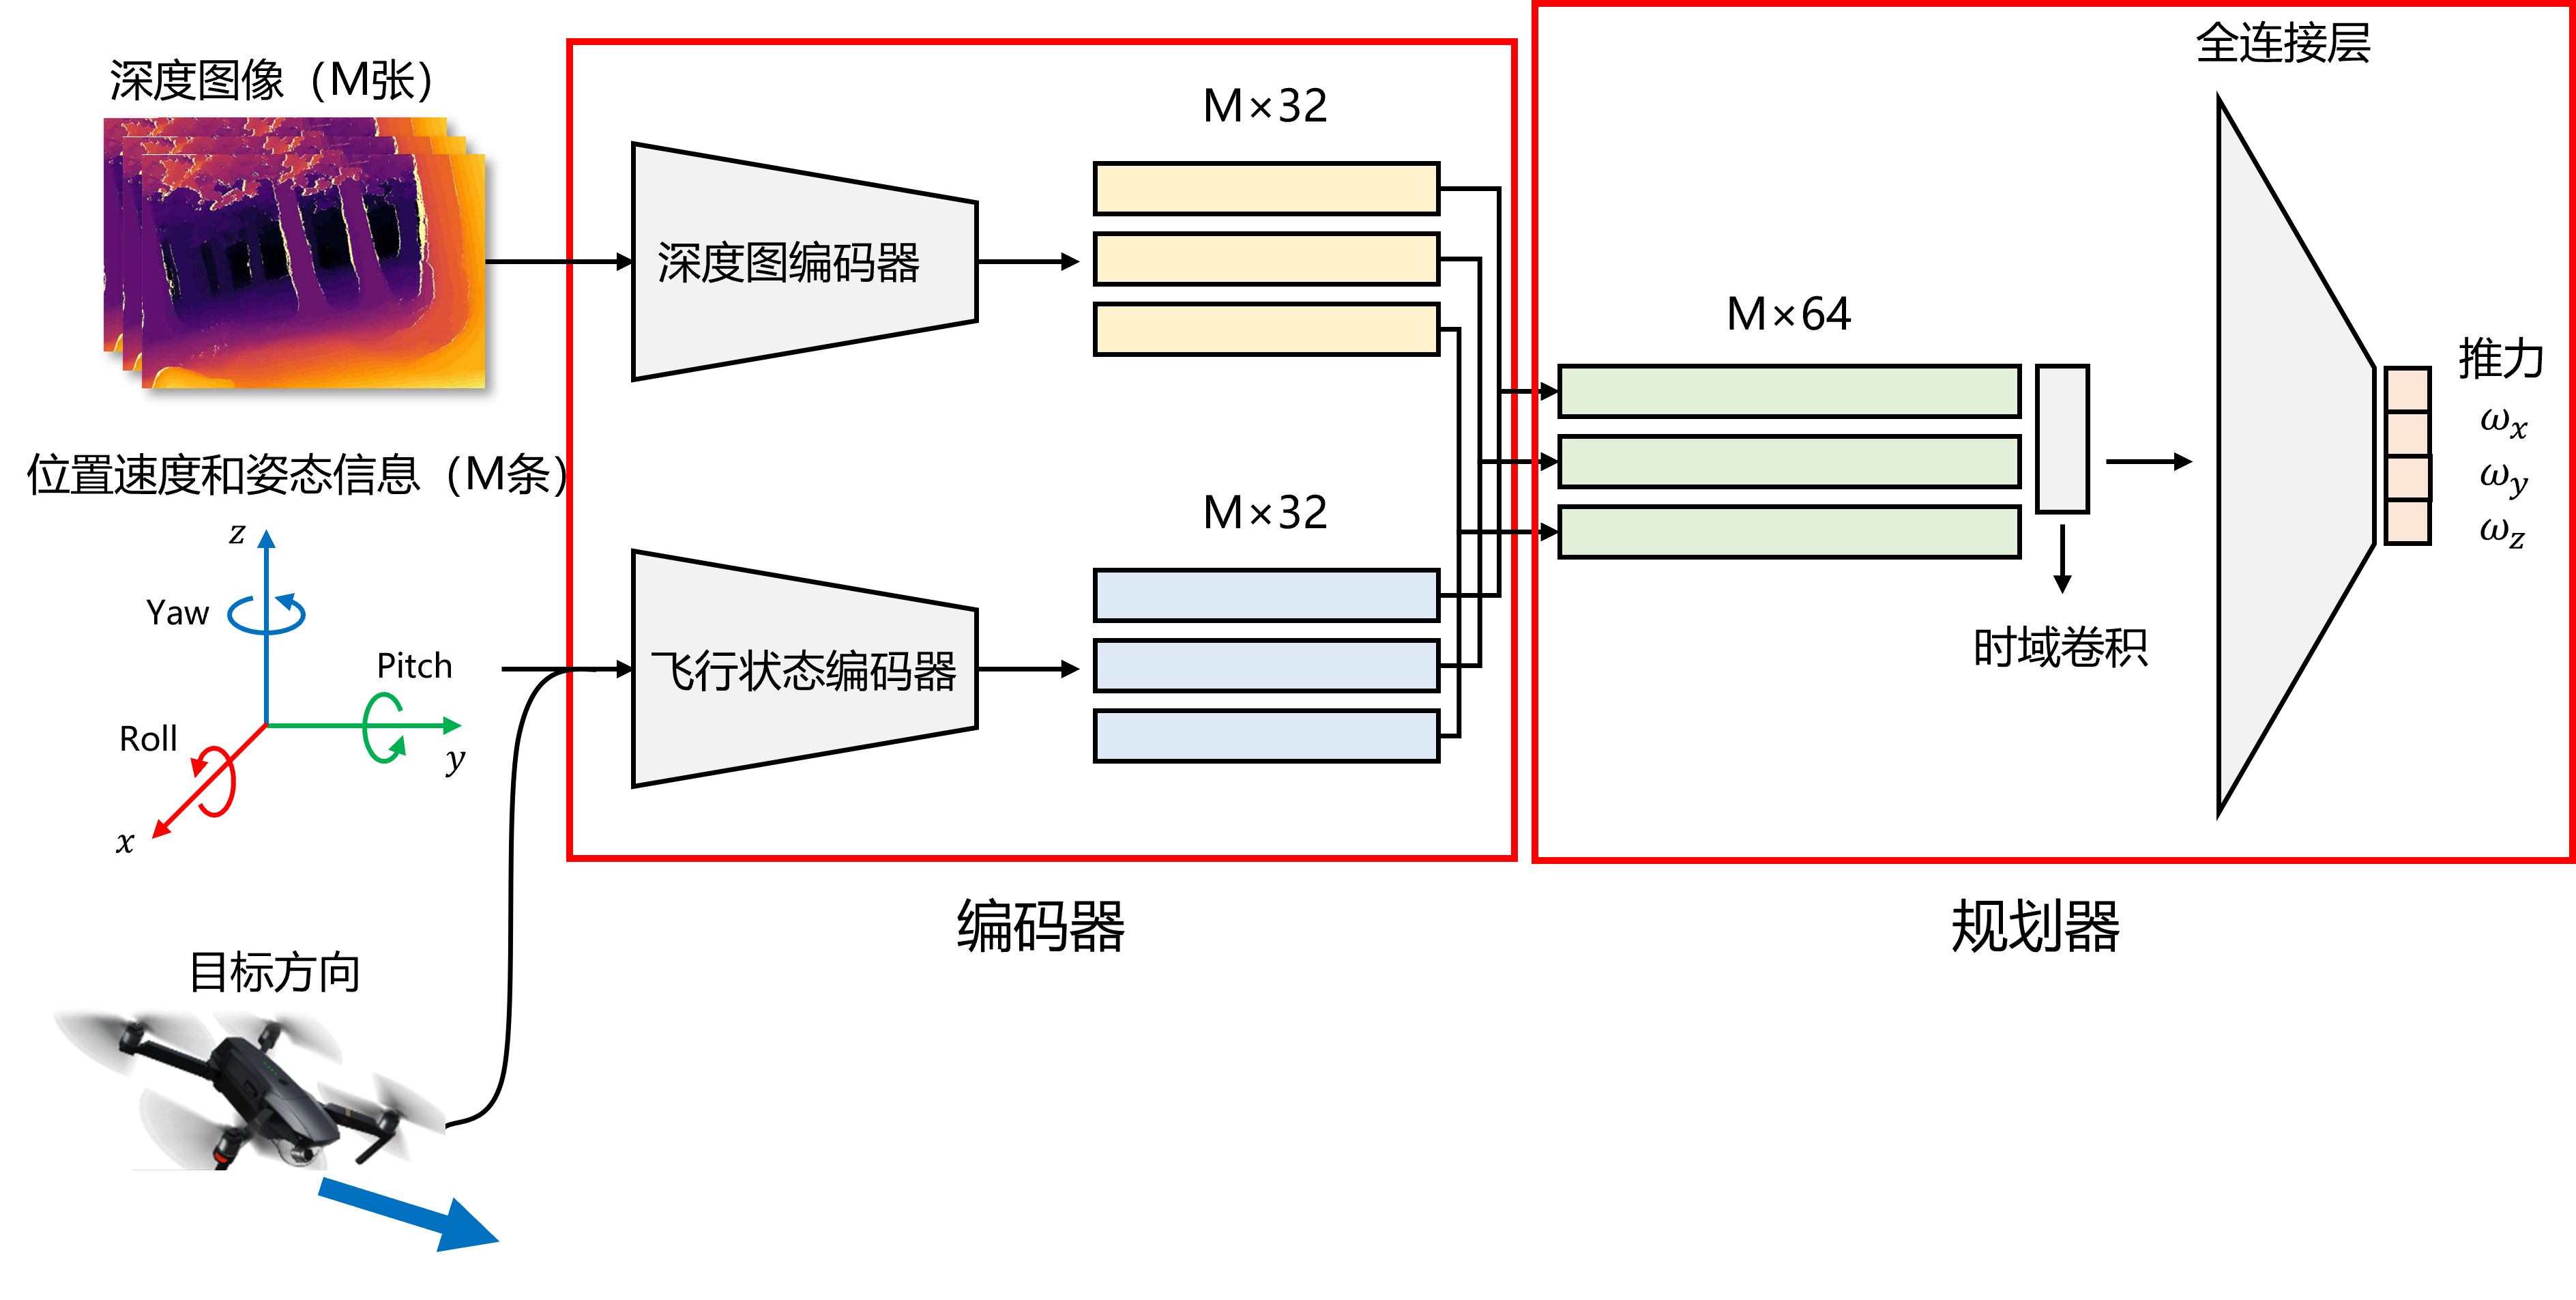
\includegraphics[width = 1\textwidth]{framework.png}
  \caption{自主导航端到端算法框架}
  \label{fig_framework}
\end{figure}

\subsection{输入和输出}
正如\ref{related_works}节所讲,无人机自主飞行任务常被划分为感知、决策、控制三部分,但实践中这样的划分往往并不绝对。为加快计算速度,本框架采用端到端的方式,将决策和部分感知、控制算法融合。框架的输入包括由IMU测量的无人机速度、加速度、角速度、角加速度;由深度相机得到的深度图,分辨率为$320\times240$像素;以及由视觉里程计(Visual-inertial odometry, VIO)输出的飞行器位置与角位置。特别地为增强算法稳定性,算法实际输入为过去一段时间的输入序列,实践中取这段序列长度为3,即$t$时刻的输入为$t-1,\ t-2,\ t-3$时刻的深度图和飞行器位置、速度、加速度信息。

企图控制一台飞行器,算法的输出也是多样的,例如飞行器的线速度和角速度、飞行器的总推力(Collective thrust)和角速度、飞行器四个旋翼的推力或转速等。相关工作表明\cite{kaufmann2022benchmark}输出为总推力与角速度(Collective thrust and body rates, CTBR)的策略往往会产生更稳健的效果,在仿真器和现实世界中的动力学差异也更小且该命令更具可解释性。因此本框架的输出为CTBR命令。在输出CTBR指令后,由飞行控制器将CTBR指令转换为四个电动机推力并执行。

\subsection{编码器(Encoder)}
\label{encoder}
无人机的输入是多模态(Multimodal)的,即包含可表达为21维向量的飞行器状态信息和可表达为320*240矩阵的深度图像,算法输入具体情况见表\ref{tab_input}。这些信息直接输入规划器可能会引起以下两个问题:
\begin{enumerate}
  \item 维度爆炸。深度图像素数量为$320\times240=76800$,维度过高,训练难度大,难以收敛。
  \item 信息不对称。深度图和飞行器状态两条输入的维度差距过大,可能会导致算法过于关注某一条输入,而忽略另一条输入。
\end{enumerate}
因此在正式输入规划器前需要两个编码器将输入信息编码为统一的维度和格式。两个编码器的结构如图\ref{fig_dep_encoder}, \ref{fig_state_encoder}中编码器部分所示。飞行状态编码器主要由时域卷积模块(Temporal Convolutional)组成,将飞行器状态信息编码时域卷积为$3*32$维。深度图编码器先经过一个MobileNetV3\cite{Howard_2019_ICCV}编码为512维向量,再通过一个时域卷积模块同样编码为$3*32$维。
\begin{table}
  \centering
  \begin{tabular}{ccccc}
  \hline
  \textbf{输入来源} & VIO & IMU & 深度相机 & 任务目标\\ \hline
  \textbf{输入形状} & 12维向量 & 6维向量 & 320*240矩阵 & 3维向量\\ \hline
      \multirow{2}*{\textbf{输入描述}} & 无人机位置3维 & \multirow{2}*{线速度与角速度} & \multirow{2}*{深度图像}  & \multirow{2}*{指向目标的单位向量}\\ 
      & 姿态旋转矩阵9维 & & \\ \hline
  \end{tabular}
  \caption{自主导航算法输入}
  \label{tab_input}
\end{table}

\begin{figure}
  \centering
  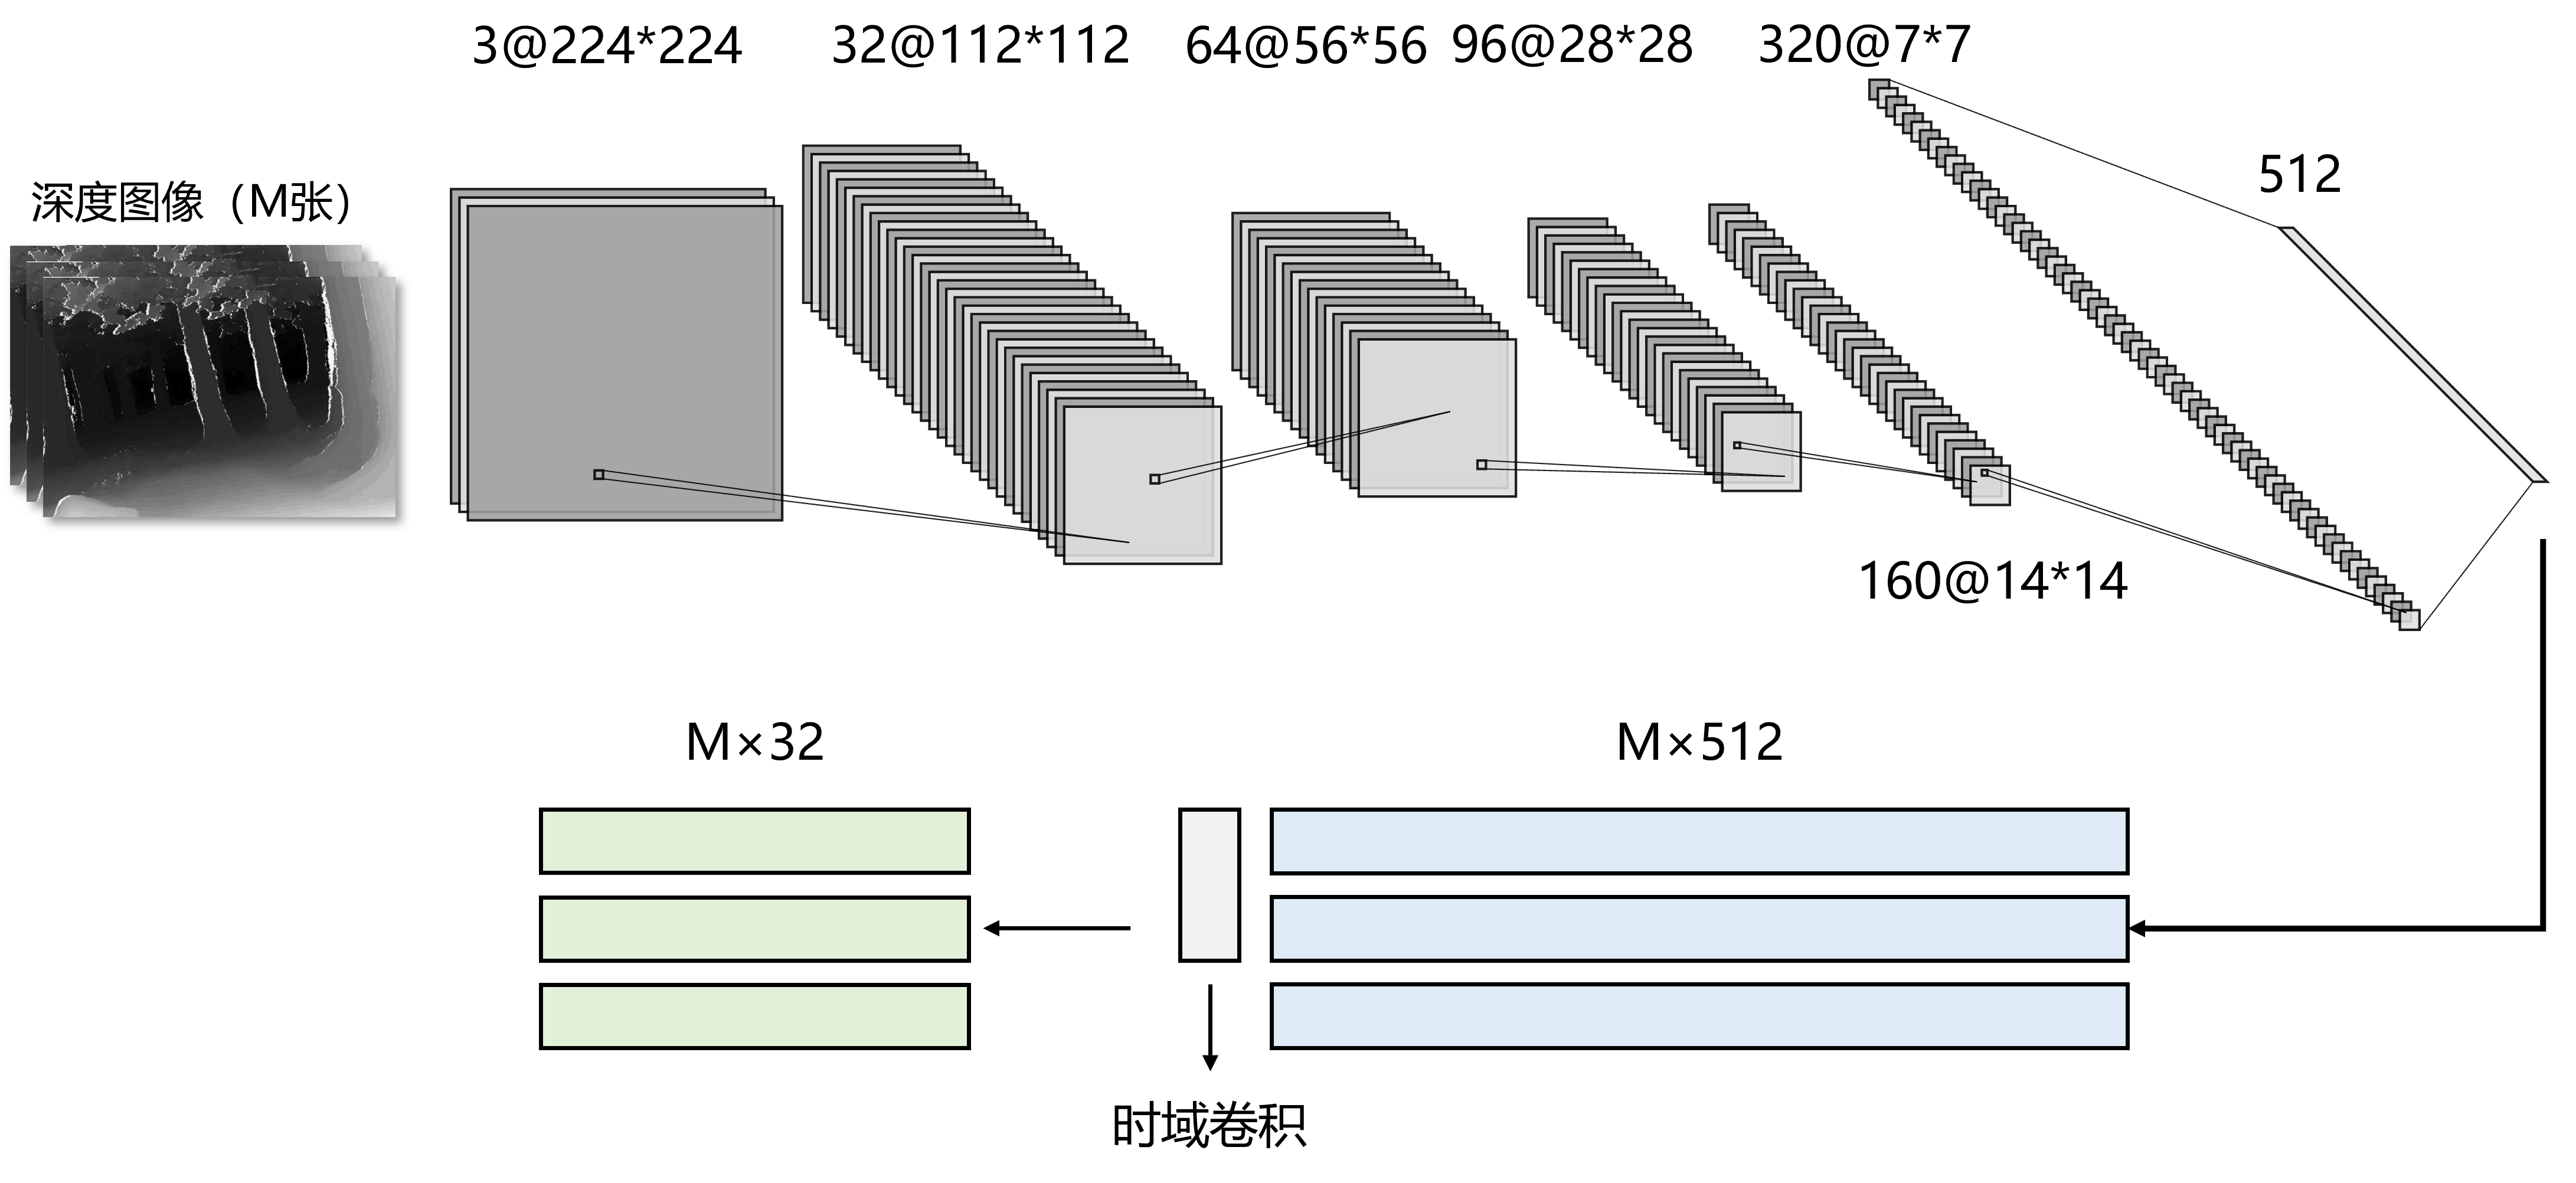
\includegraphics[width = 1\textwidth]{dep_encoder.png}
  \caption{深度图编码器结构图}
  \label{fig_dep_encoder}
\end{figure}

\begin{figure}
  \centering
  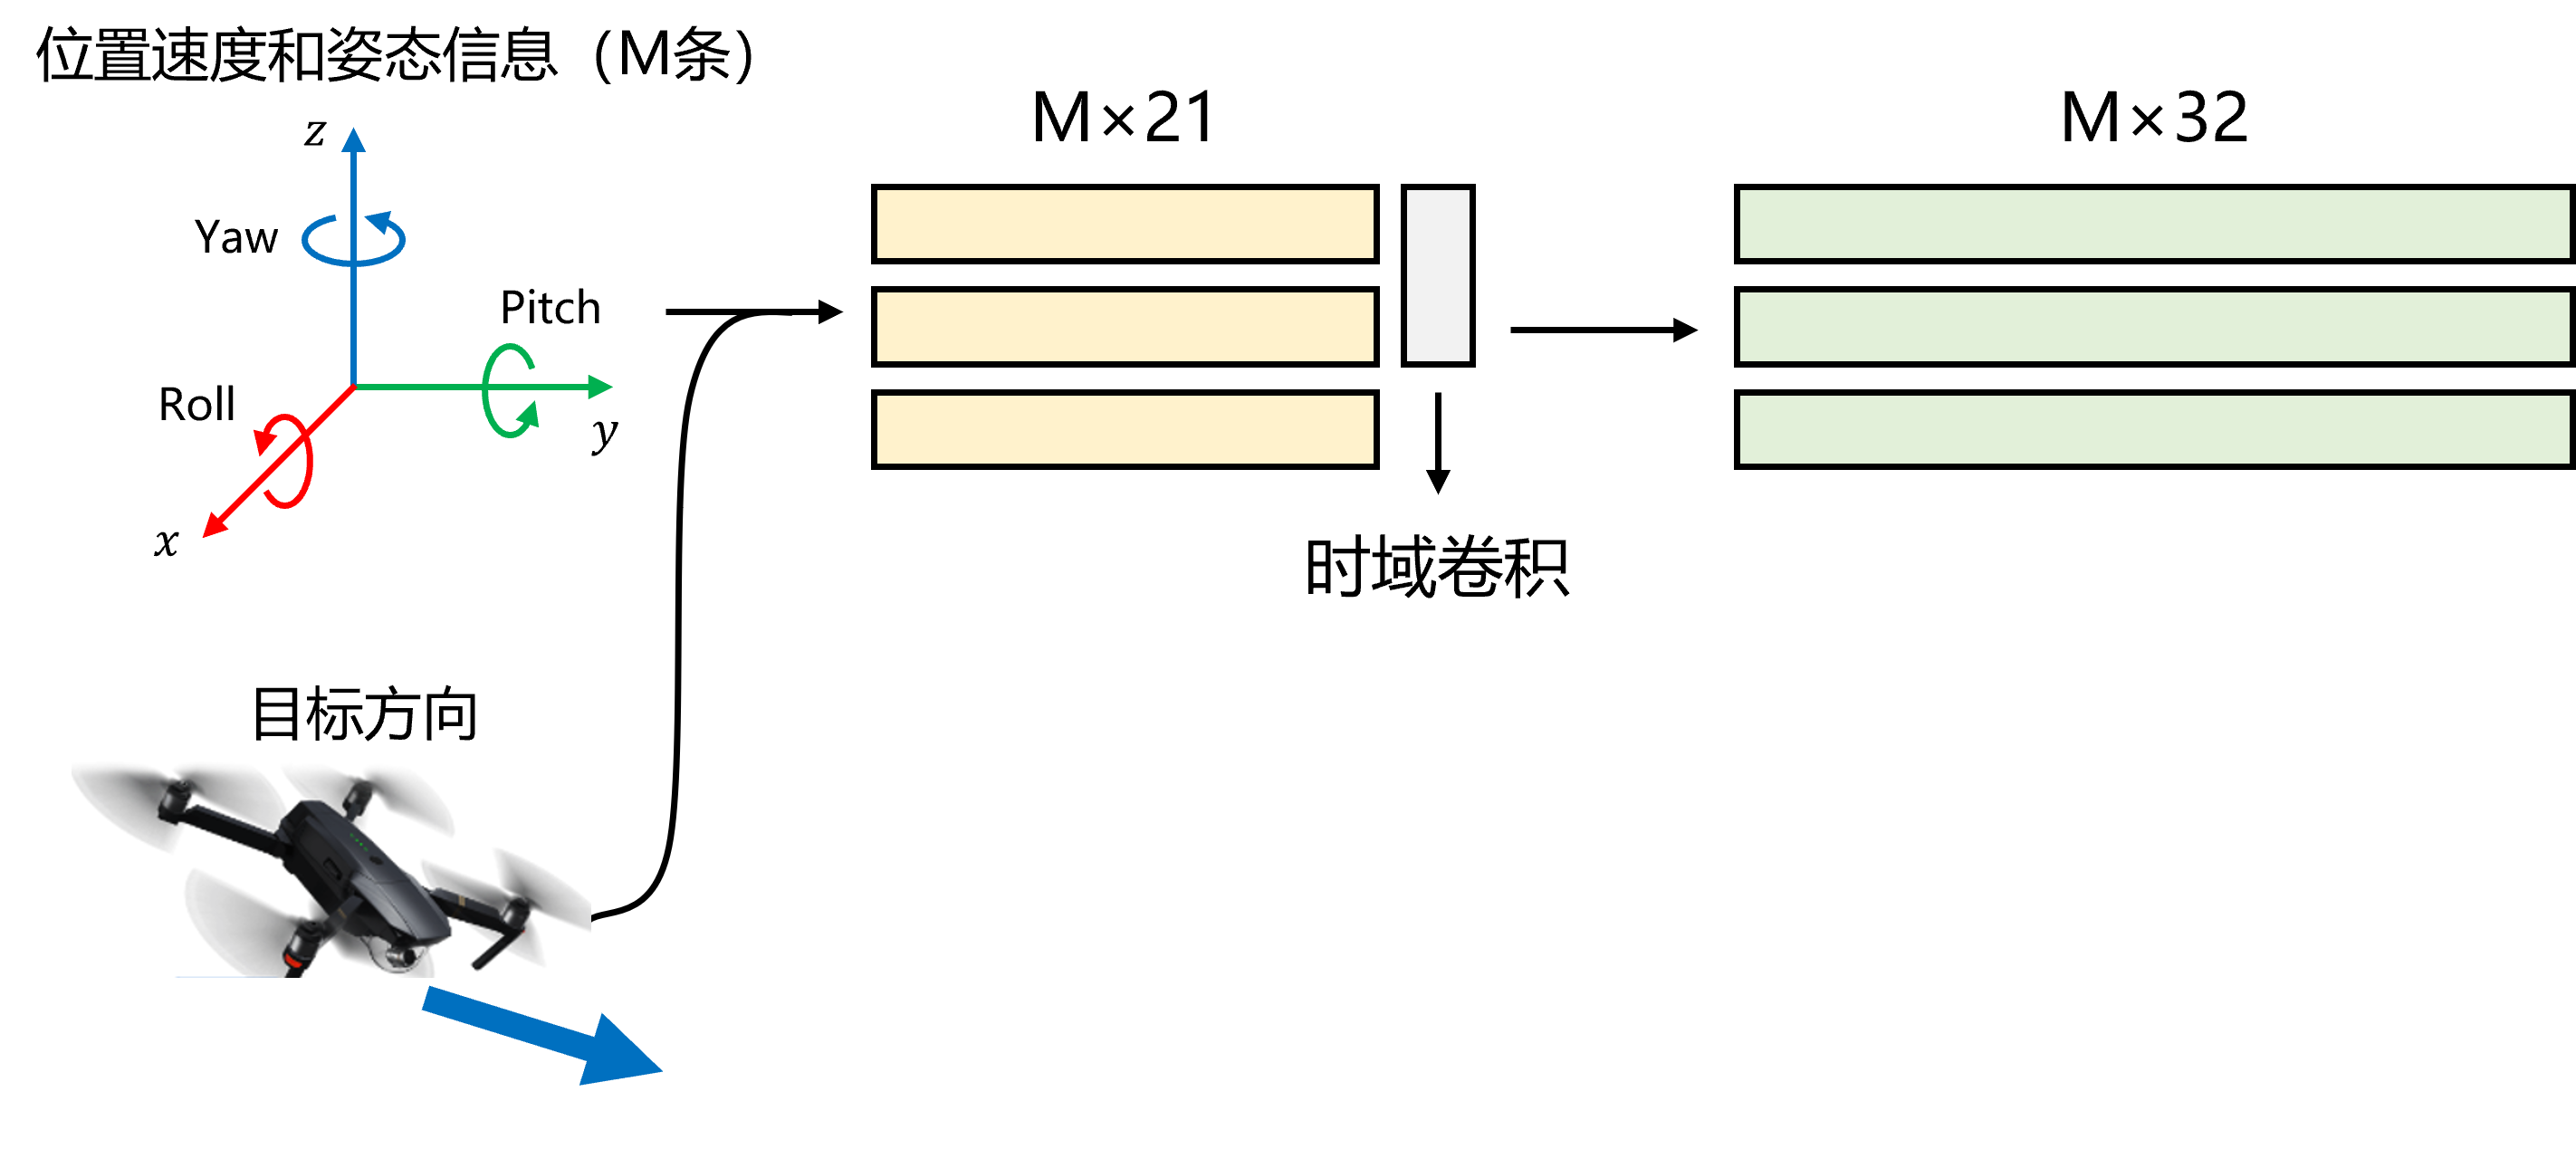
\includegraphics[width = 0.8\textwidth]{state_encoder.png}
  \caption{飞行状态编码器结构图}
  \label{fig_state_encoder}
\end{figure}

\subsection{规划器(Planner)}
将编码器编码过的两个$3*32$维的矩阵拼接为$3*64$维的矩阵,作为规划器的输入。规划器的结构如图\ref{fig_planner}所示,由一个时域卷积模块和一个全连接层组成。在时域再次进行卷积后输入全连接层,经过$[512, 256, 128, 64]$节点的四个隐藏层后输出为$4$维,分别表示CTBR四个维度的指令。规划器的输出会被送入飞行控制器,由飞行控制器将CTBR指令转换为四个电动机推力并执行。
\begin{figure}
  \centering
  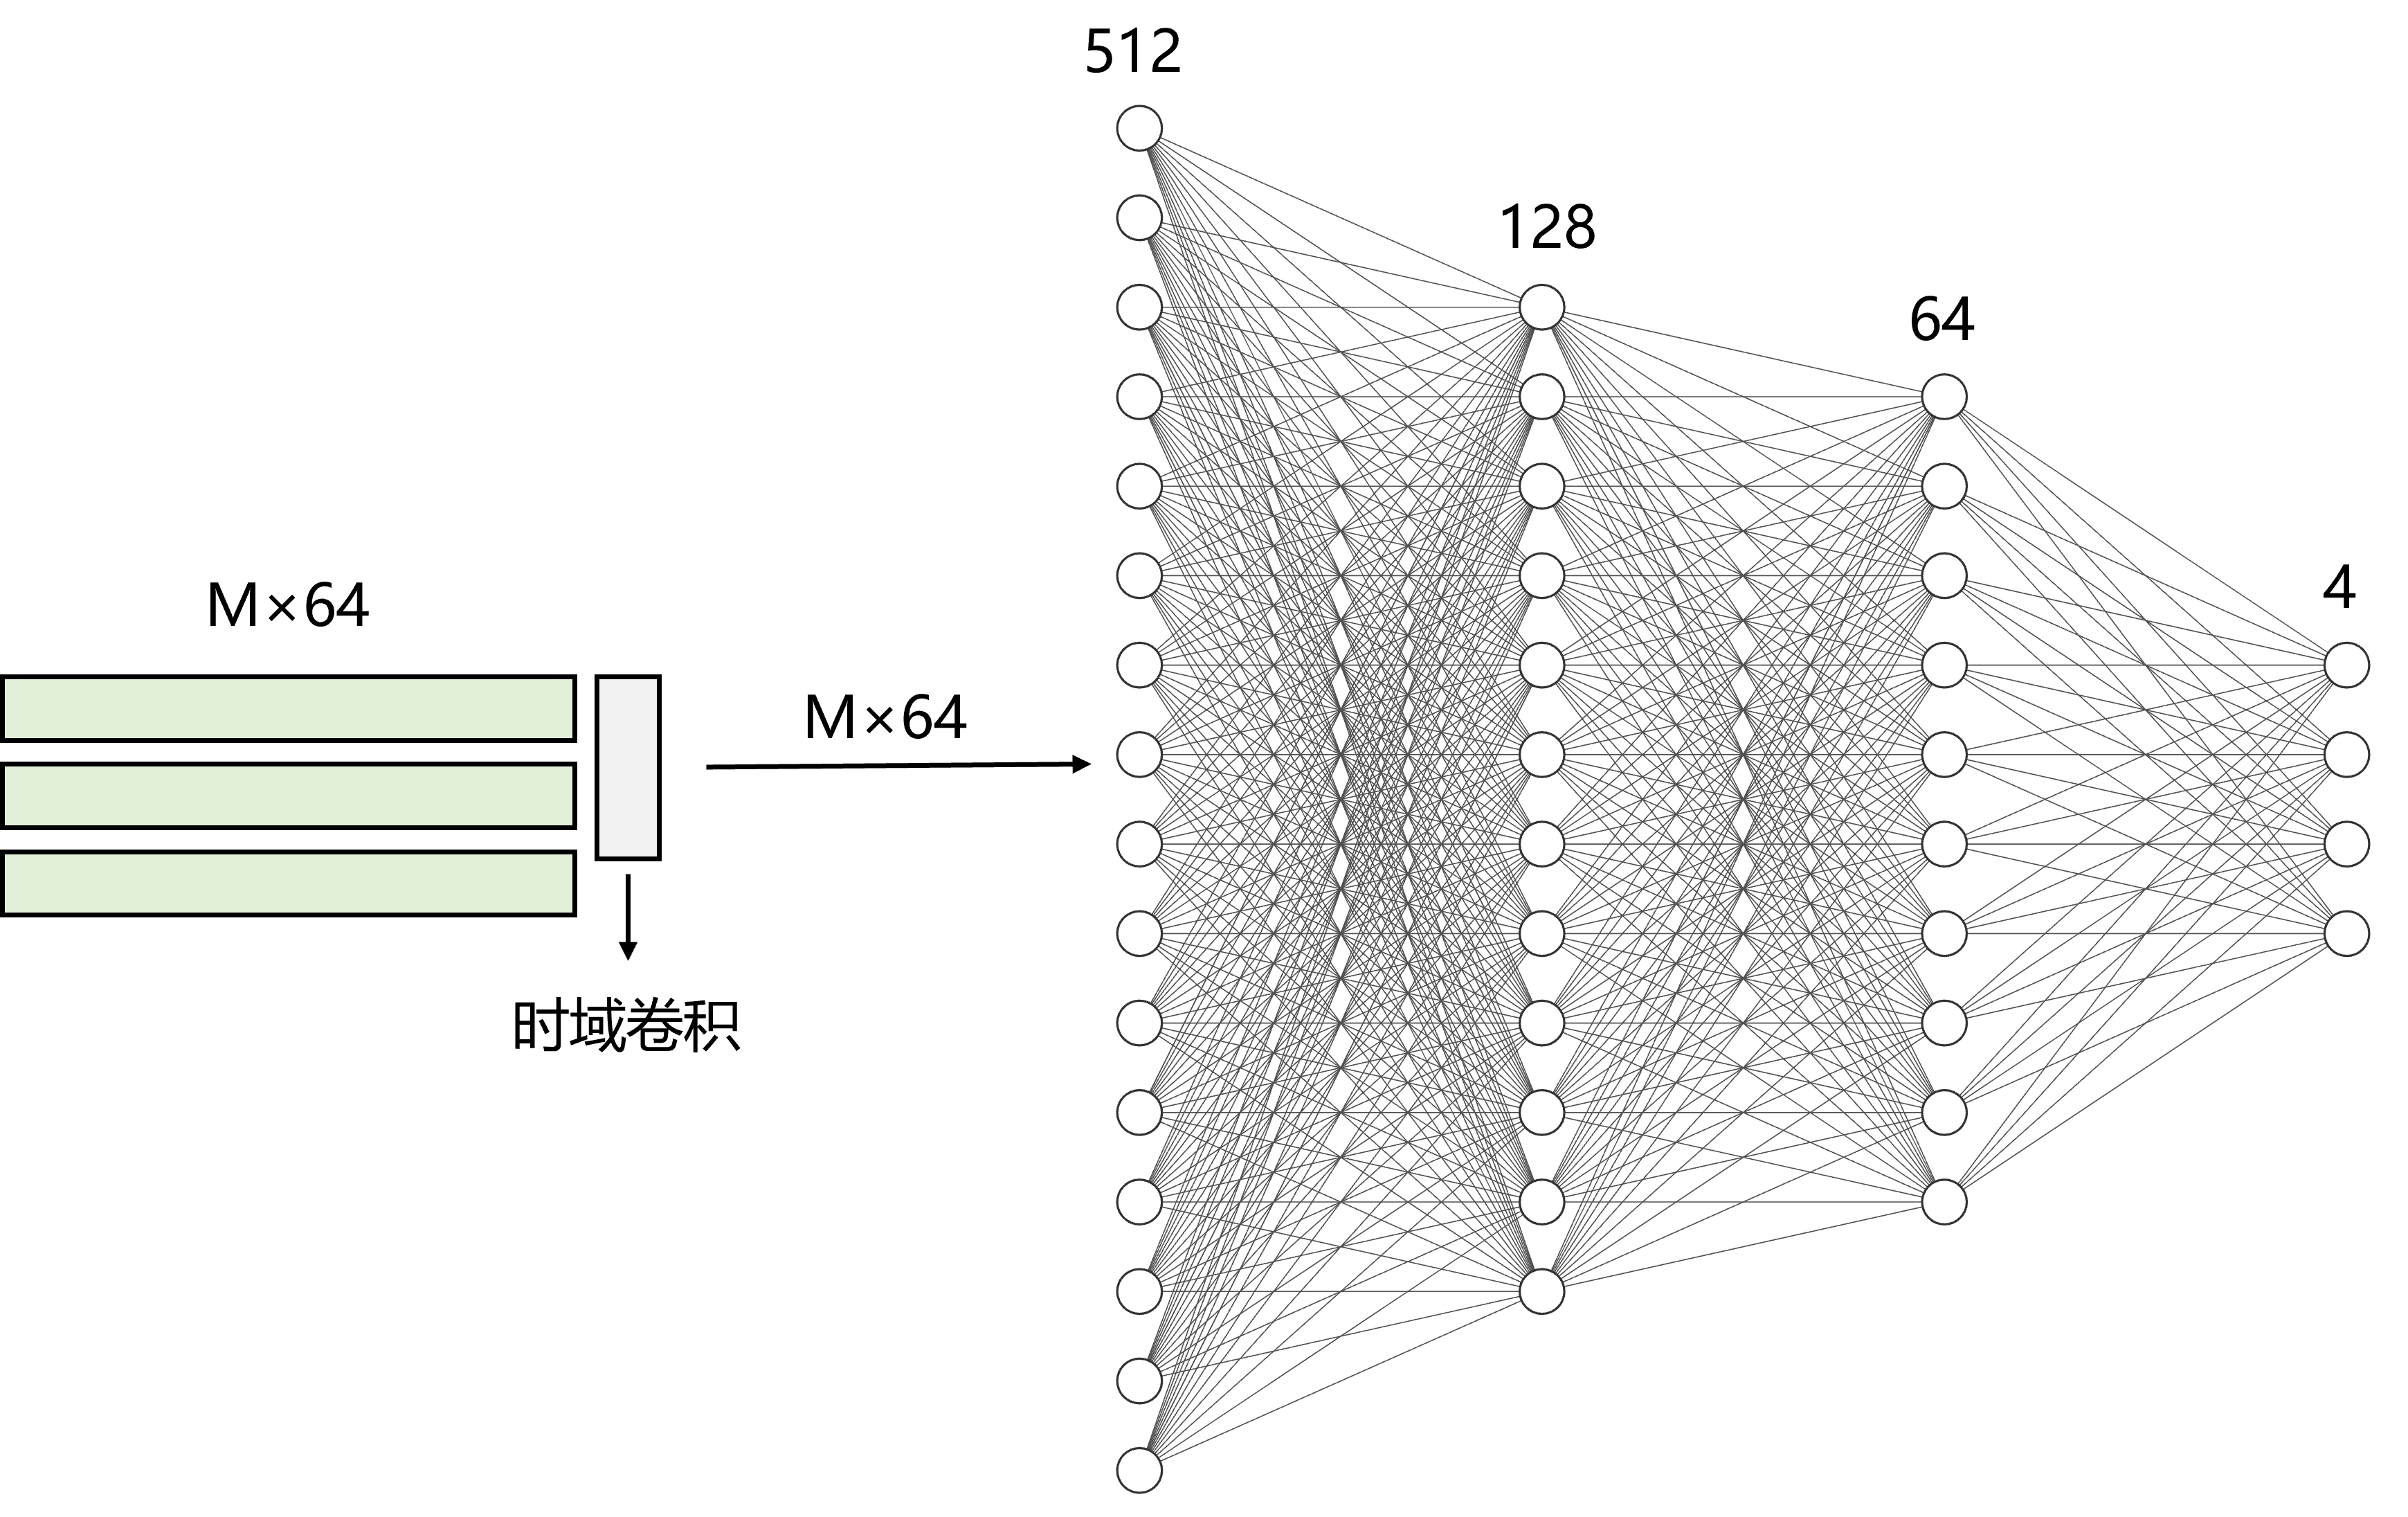
\includegraphics[width = 0.9\textwidth]{planner.png}
  \caption{规划器结构图}
  \label{fig_planner}
\end{figure}
经过实验与调研\cite{loquercio2021learning},该端到端框架相比传统感知-建图-规划的方法执行速度更快,与其它基于学习的方法执行速度类似,测试结果如表\ref{tab_exetime}所示。

\begin{table}
  \centering
  \begin{tabular}{ccccc}
  \hline
      \textbf{方法} & \textbf{阶段} & \textbf{用时(ms)} & \textbf{占比} & \textbf{总用时} \\ \hline
      \multirow{3}*{FastPlanner\cite{zhou2019robust}} & 预处理 & 14.6 & 22.4\% & \multirow{3}*{65.2} \\ %\cline{2-4}
      ~ & 建图 & 49.2 & 75.5\% & ~ \\ %\cline{2-4}
      ~ & 规划 & 1.4 & 2.1\% & ~ \\ \hline
      \multirow{2}*{Reactive\cite{florence2020integrated}} & 预处理 & 13.8 & 72.3\% & \multirow{2}*{19.1} \\ %\cline{2-4}
      ~ & 规划 & 5.3 & 27.7\% & ~ \\ \hline
      \multirow{3}*{Learning Planner\cite{loquercio2021learning}} & 预处理 & 0.1 & 1\% & \multirow{3}*{10.3} \\ 
      ~ & 神经网络推理 & 10.1 & 98\% & ~ \\ 
      ~ & 规划 & 0.08 & 1\% & ~ \\ \hline
      \multirow{2}*{本方法} & 预处理 & 0.1 & 1\% & \multirow{2}*{13.3} \\ 
      ~ & 神经网络推理 & 13.2 & 99\% & ~ \\ \hline
  \end{tabular}
  \caption{各自主导航算法执行时间}
  \caption*{测试平台为Intel Core i7-8700K CPU, NVIDIA GeForce RTX 2080 GPU}
  \label{tab_exetime}
\end{table}

\section{训练方法}
\subsection{三段式训练方法}
将自主导航算法整体接入仿真器训练,经测试训练各模块运行频率如表\ref{train_freq}所示。Unity渲染深度图像运行频率慢,成为训练瓶颈。为此本研究提出了三段式训练方法,主要思路是在在线(Online)强化学习阶段使用更快速获取的信息(点云)作为输入以避免渲染深度图像对训练速度的影响。具体地,三段式训练方法如图\ref{fig_step1}\ref{fig_step2}\ref{fig_step3}所示。第一阶段需在采集好的点云数据集上使用自动编码器 (Autoencoder)的方法训练点云编码器。第二阶段将预训练的点云编码器和点云输入接入规划器,进行在线强化学习训练。第三阶段再采集点云-深度图像数据对,有监督地训练深度图编码器。在部署时仅需要接入分别在第二、三步训练好的深度图编码器和规划器即可。下面将分别详细介绍这三个步骤。
\begin{table}
  \centering
  \begin{tabular}{ccccc}
      \hline
      \textbf{仿真模块} & \textbf{Unity渲染深度图} & \textbf{Gazebo动力学模拟} & \textbf{控制器} & \textbf{神经网络推理} \\ \hline
      运行频率(Hz) & 15$\sim$30 & 2000 & $>$1000 & $>$300 \\ \hline
  \end{tabular}
  \caption{仿真器各模块运行频率}
  \caption*{测试平台为Intel Core i9-13900K CPU, NVIDIA GeForce RTX 4090 GPU}
  \label{train_freq}
\end{table}

\begin{figure}
  \centering
  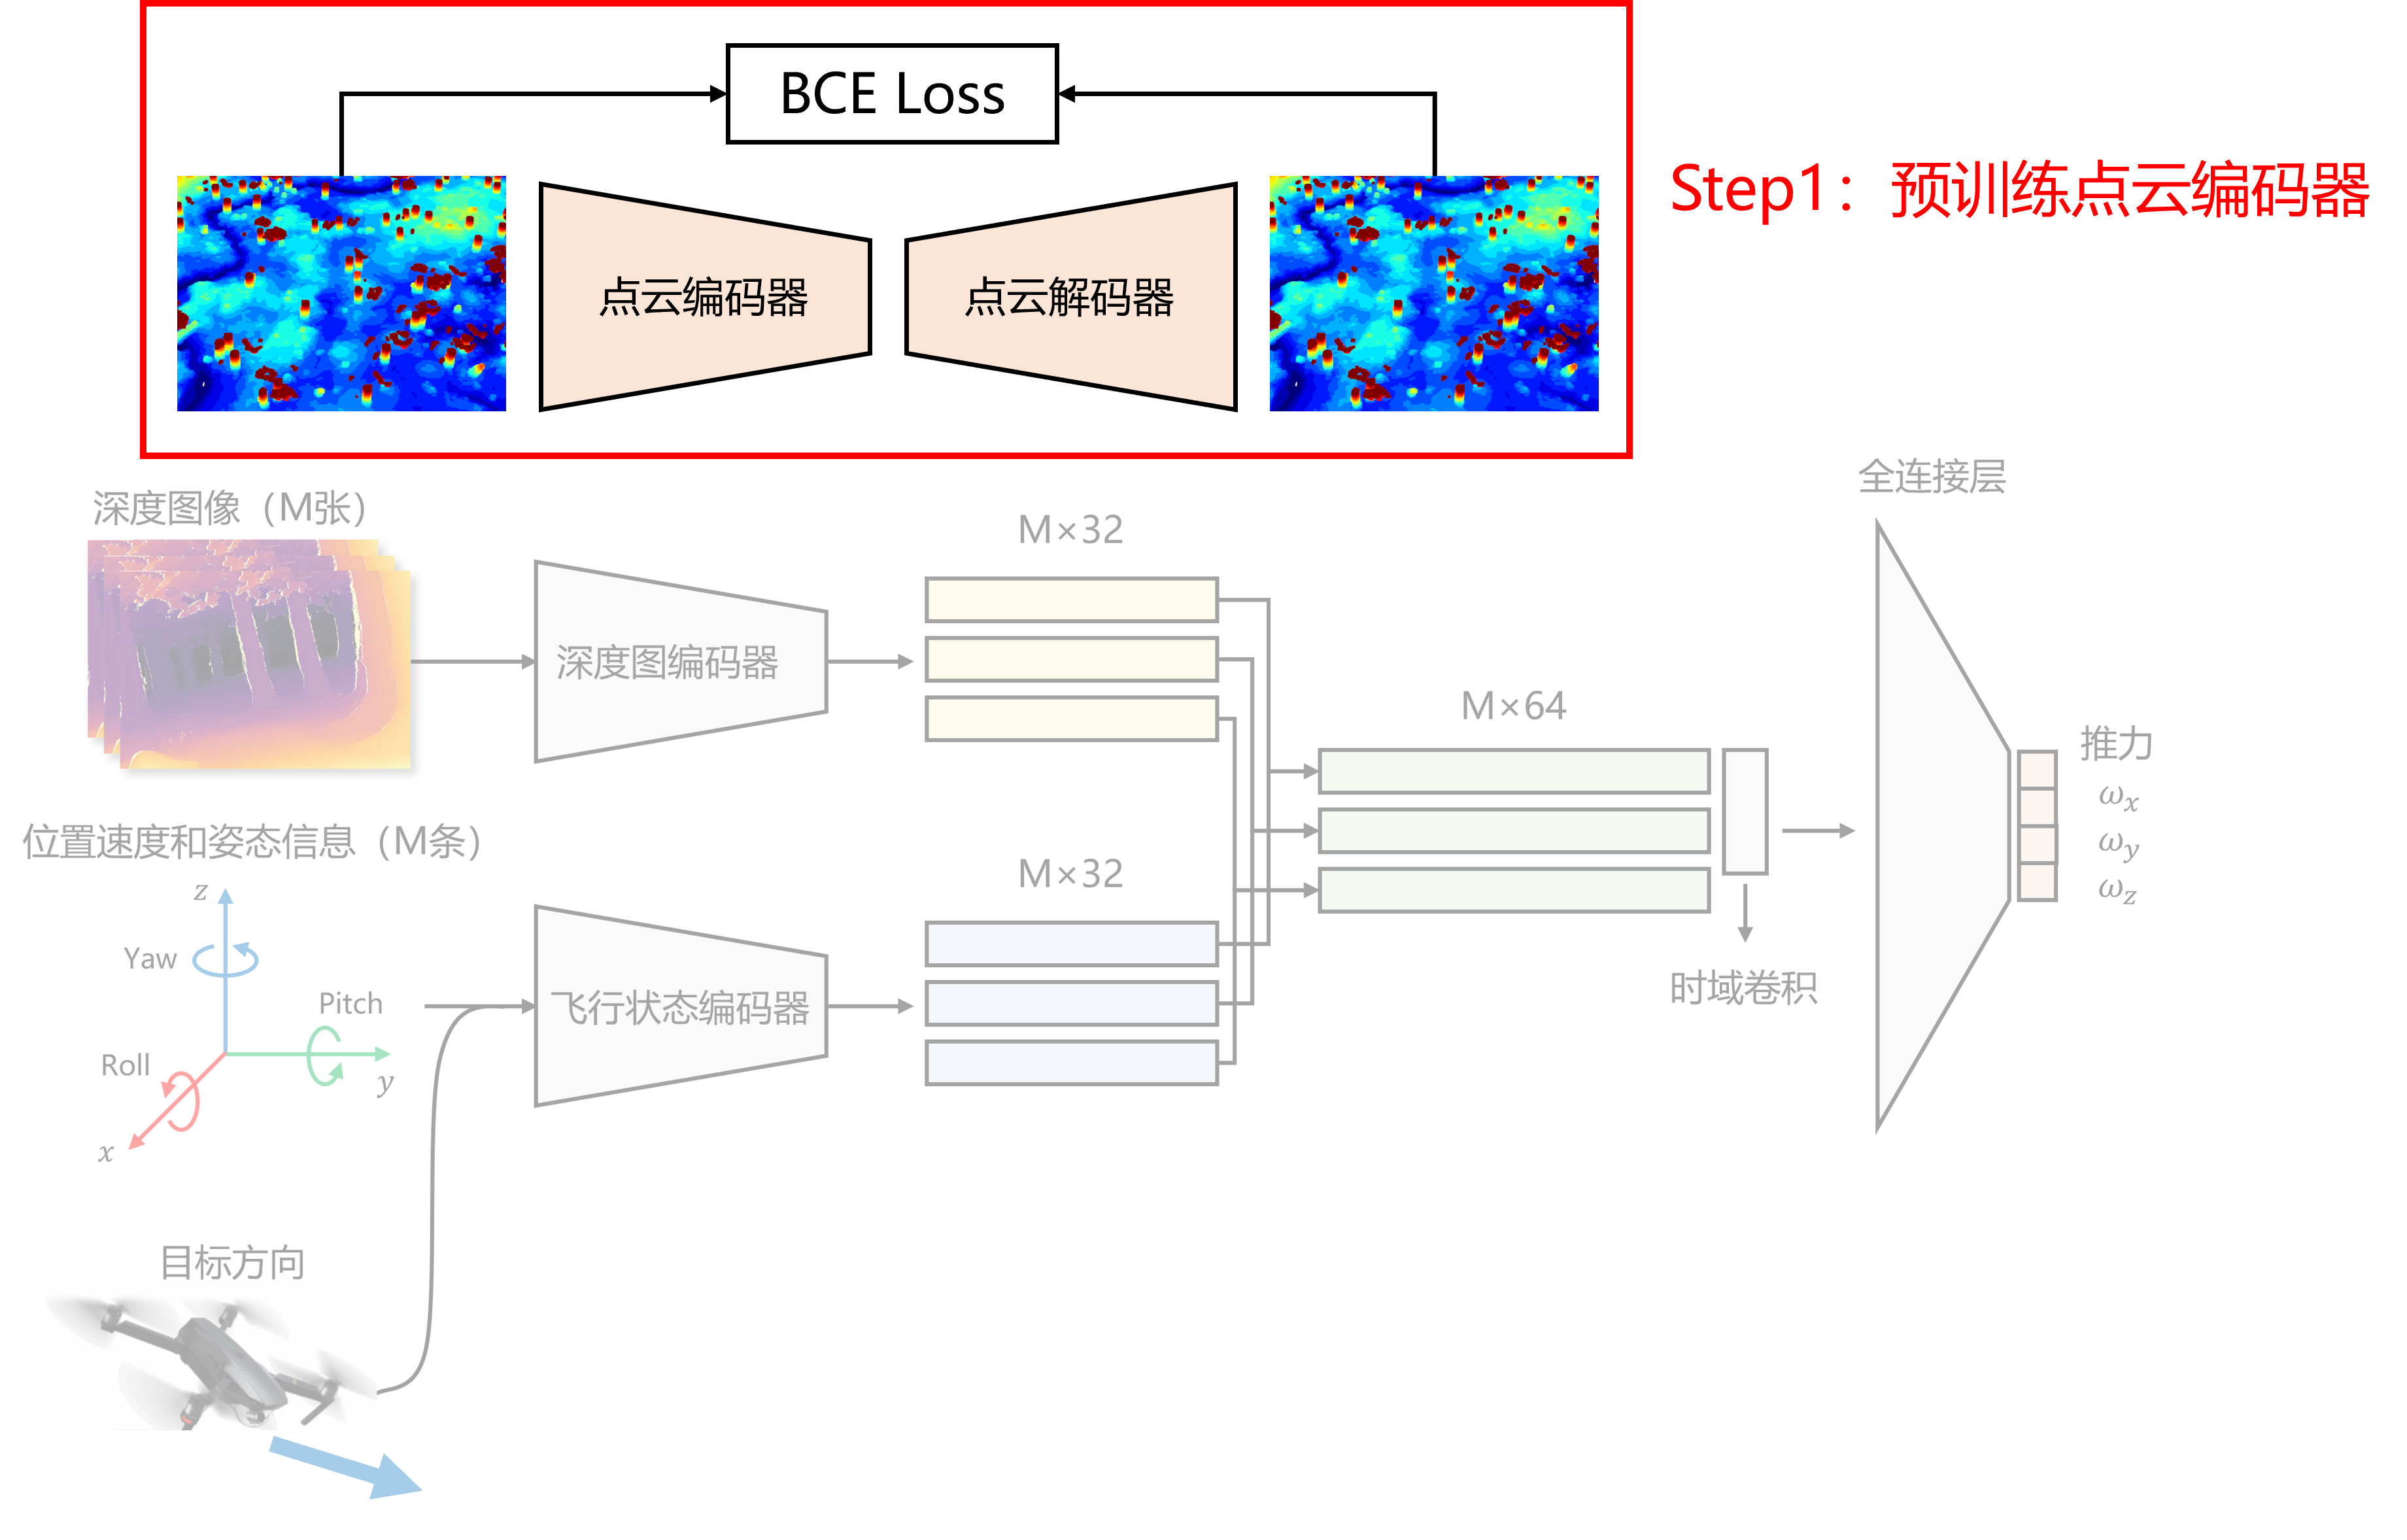
\includegraphics[width = 0.95\textwidth]{step1.png}
  \caption{预训练点云编码器}
  \label{fig_step1}
\end{figure}

\begin{figure}
  \centering
  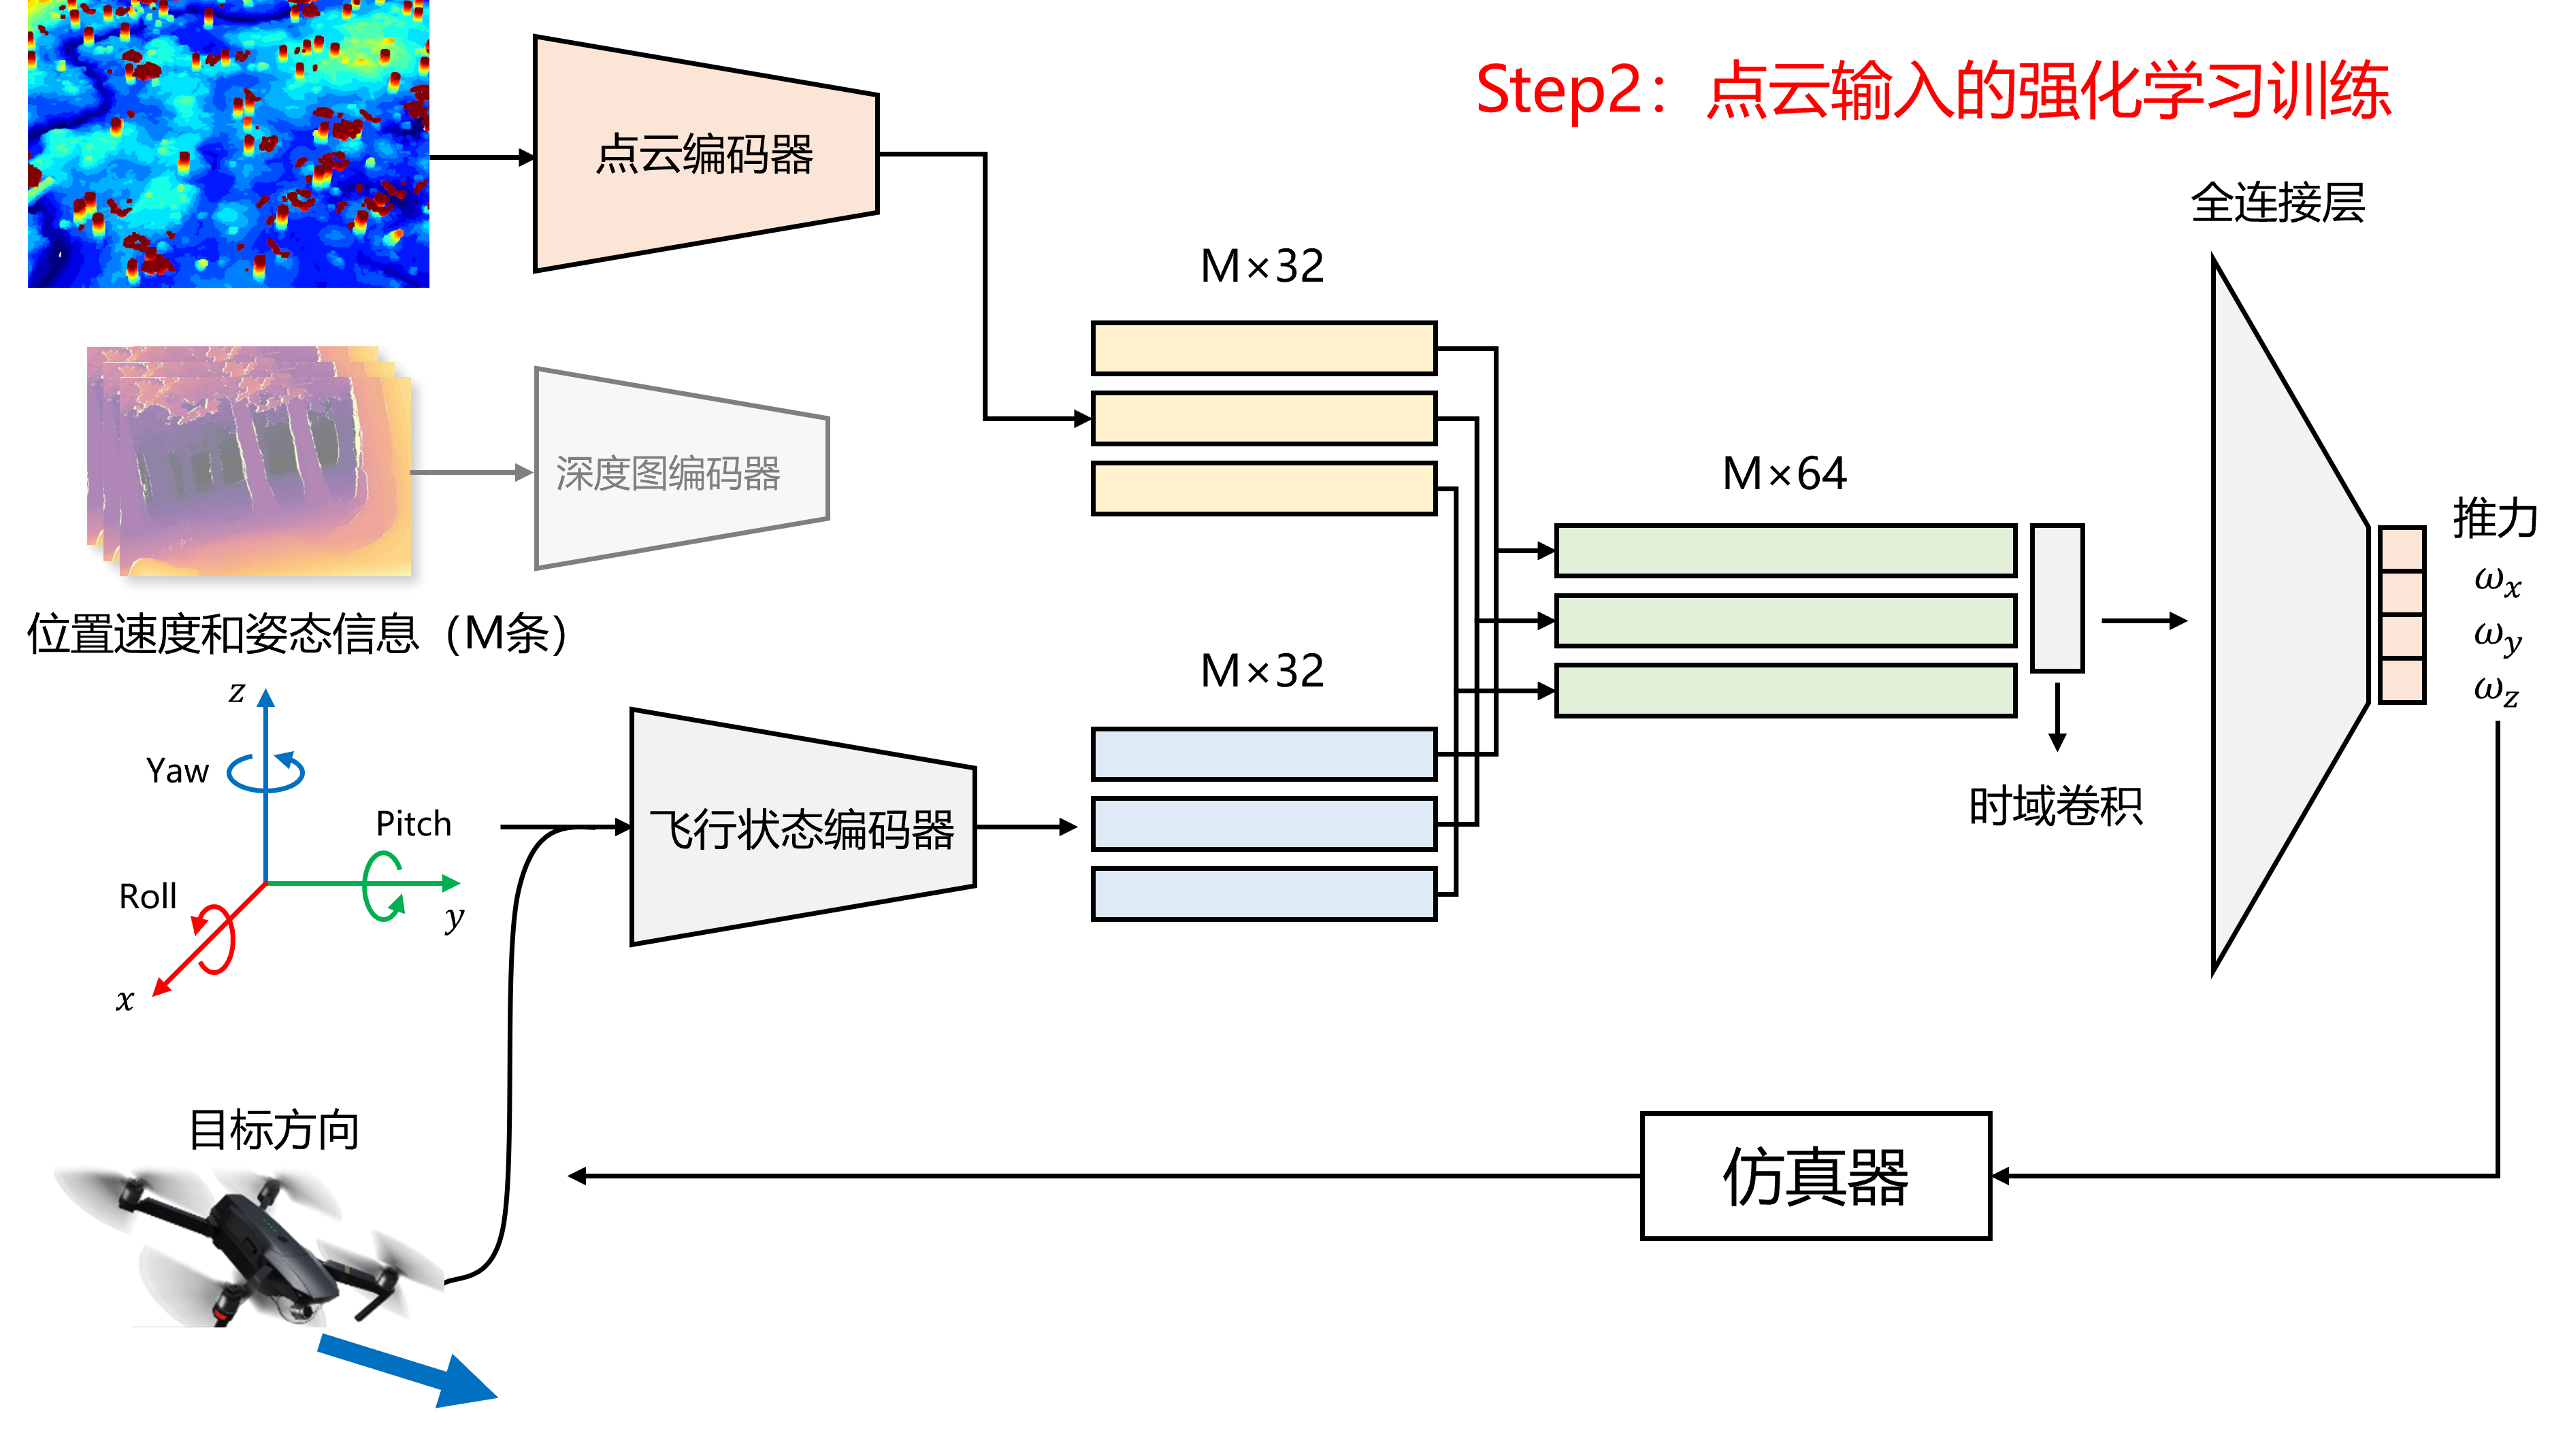
\includegraphics[width = 1\textwidth]{step2.png}
  \caption{点云输入的强化学习训练}
  \label{fig_step2}
\end{figure}

\begin{figure}
  \centering
  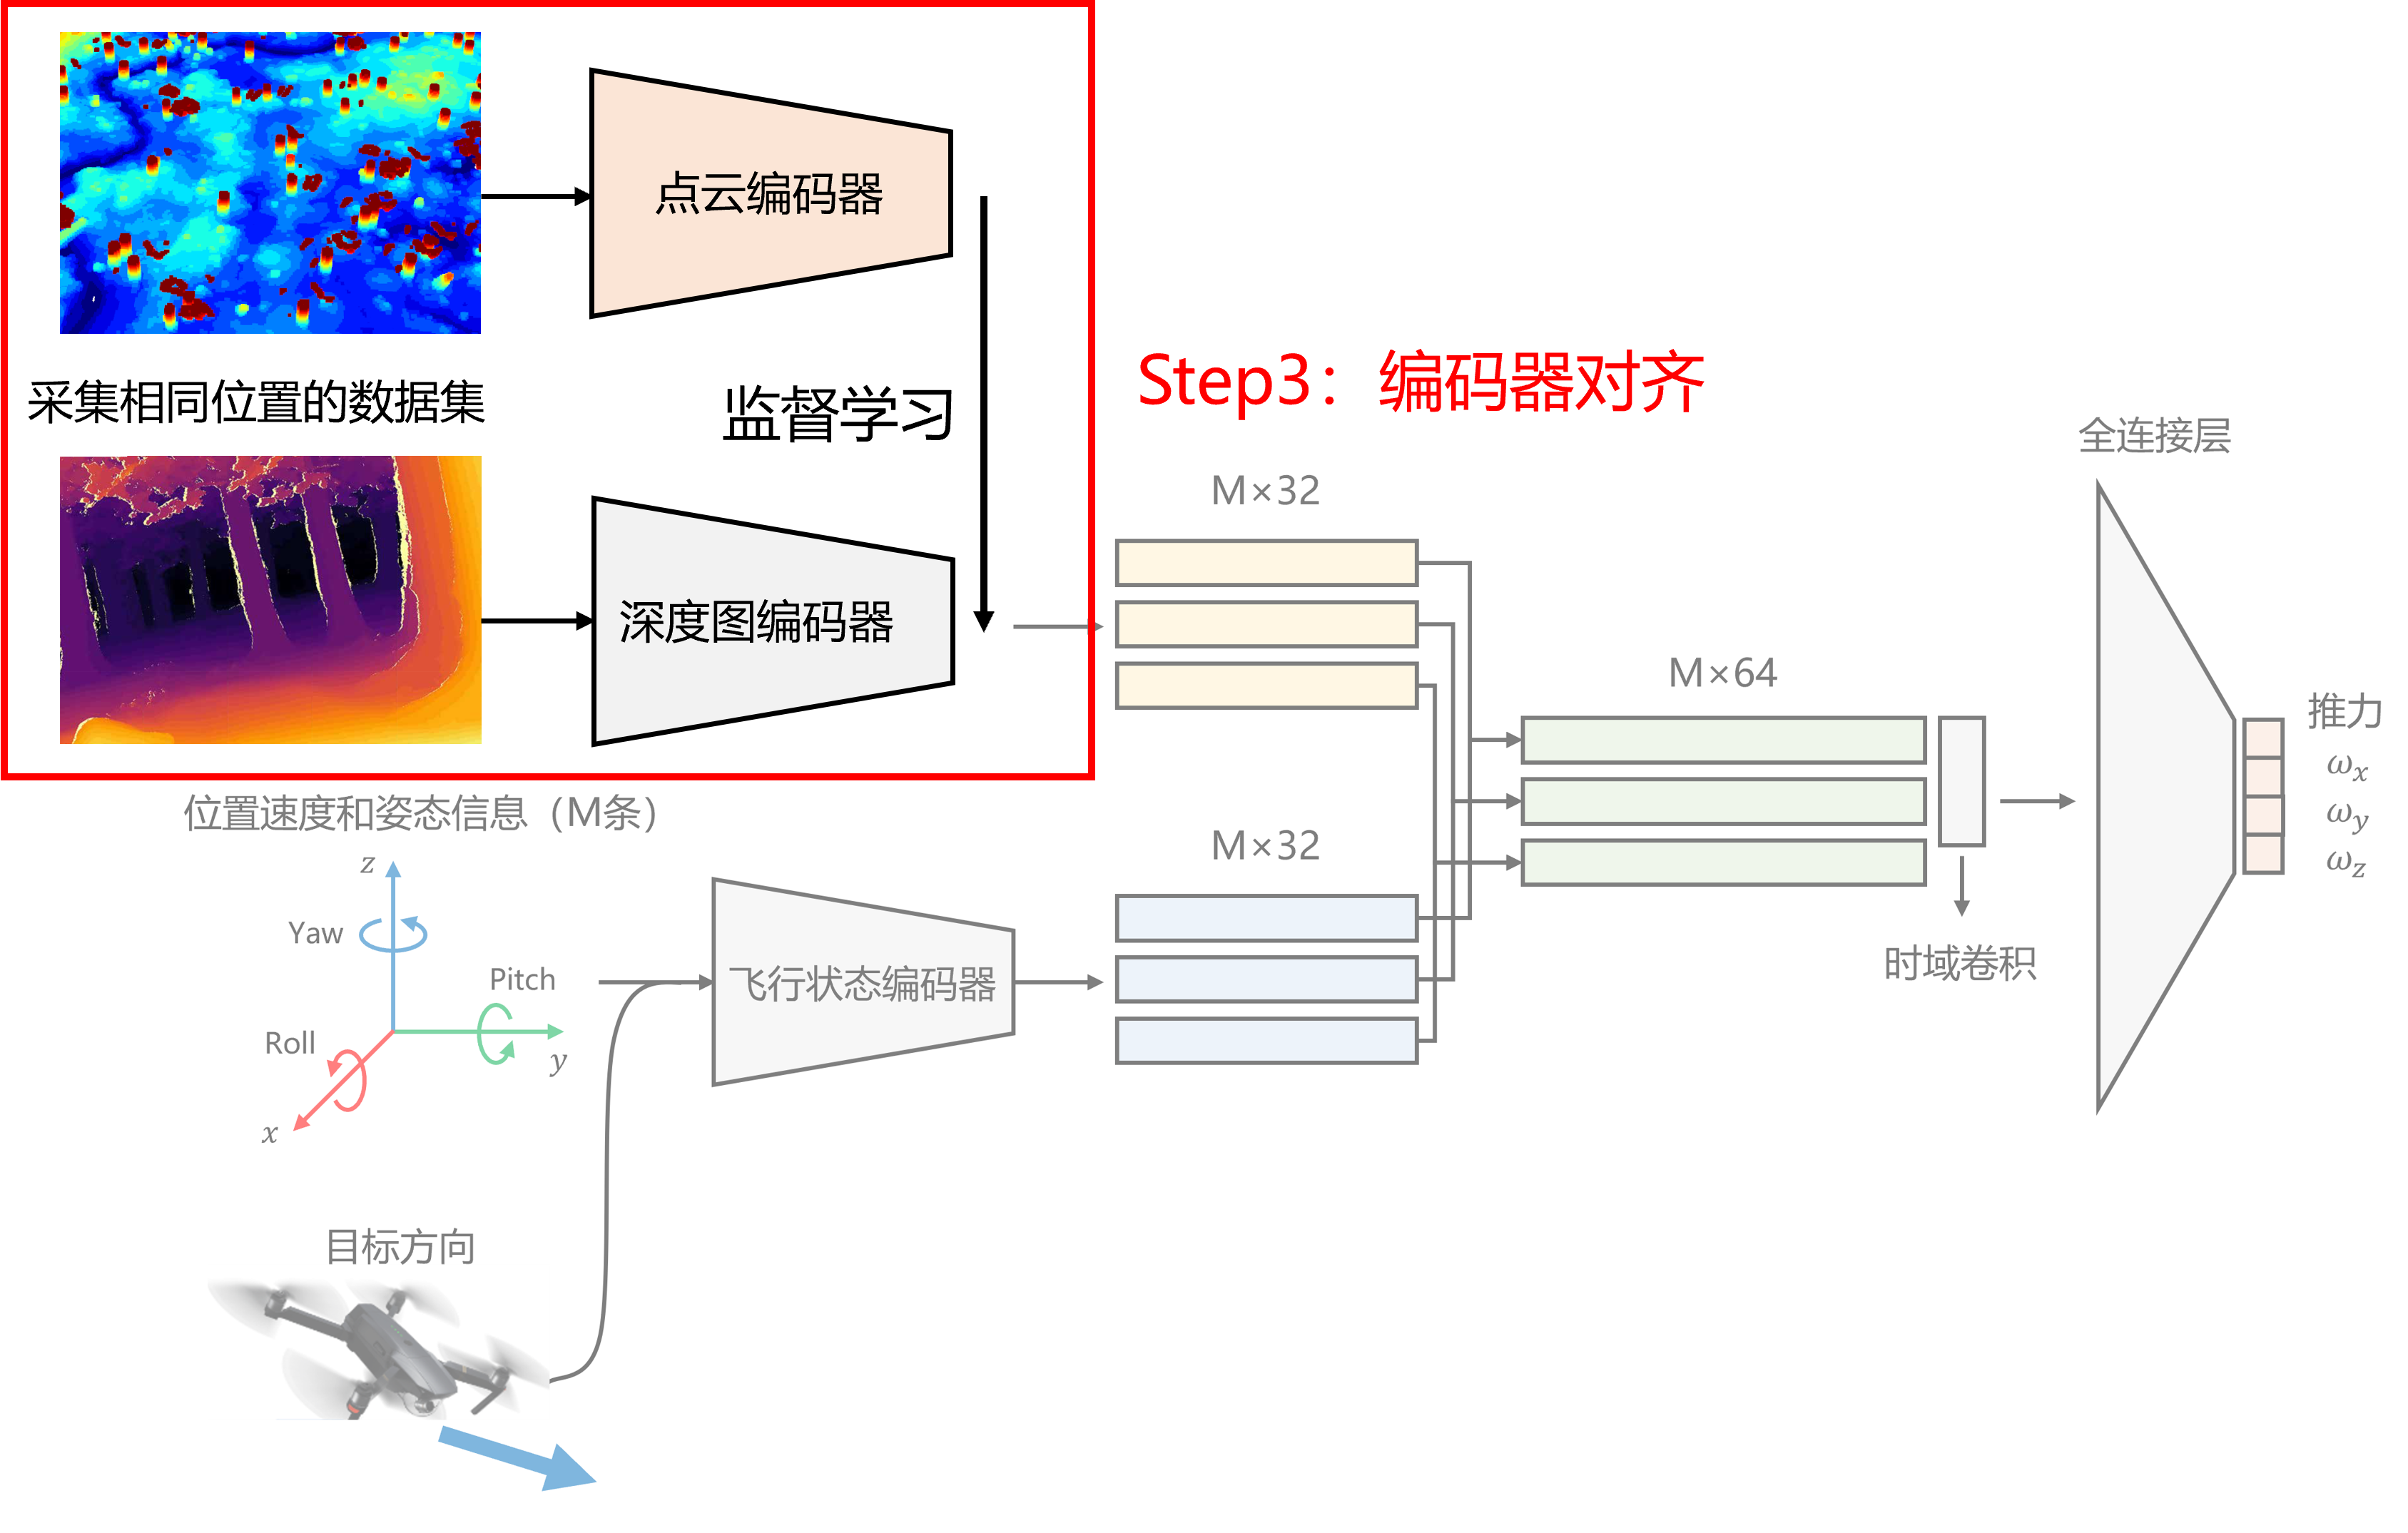
\includegraphics[width = 0.89\textwidth]{step3.png}
  \caption{编码器对齐}
  \label{fig_step3}
\end{figure}

\subsubsection{预训练点云编码器}
同\ref{encoder}节所讲,以点云为输入的训练同样需要点云编码器。虽然无人机自主导航任务的环境是未知的,但环境的类型和大体分布是已知的。我们预渲染了几百幅地图的点云数据,从中随机裁剪(Crop)大小与深度相机感知范围一致,即$3m\times 3m\times 2m$的点云块。这些随机采集的点云块数据集与飞行中可能遇到的点云输入是类似的,因此可以在点云块数据集上训练点云编码器,如图\ref{fig_step1}。点云编码器的结构如图\ref{fig_pcd_encoder}所示,在其后接入与编码器对应的解码器(Decoder)以重建输入点云块。训练使用二进制交叉熵(Binary cross entropy, BCE)损失函数,将解码器重建的点云块与原始点云块对比做自监督训练。训练完成后,点云编码器可以将点云块编码为512维的向量,该向量就可作为规划器的输入。

\begin{figure}
  \centering
  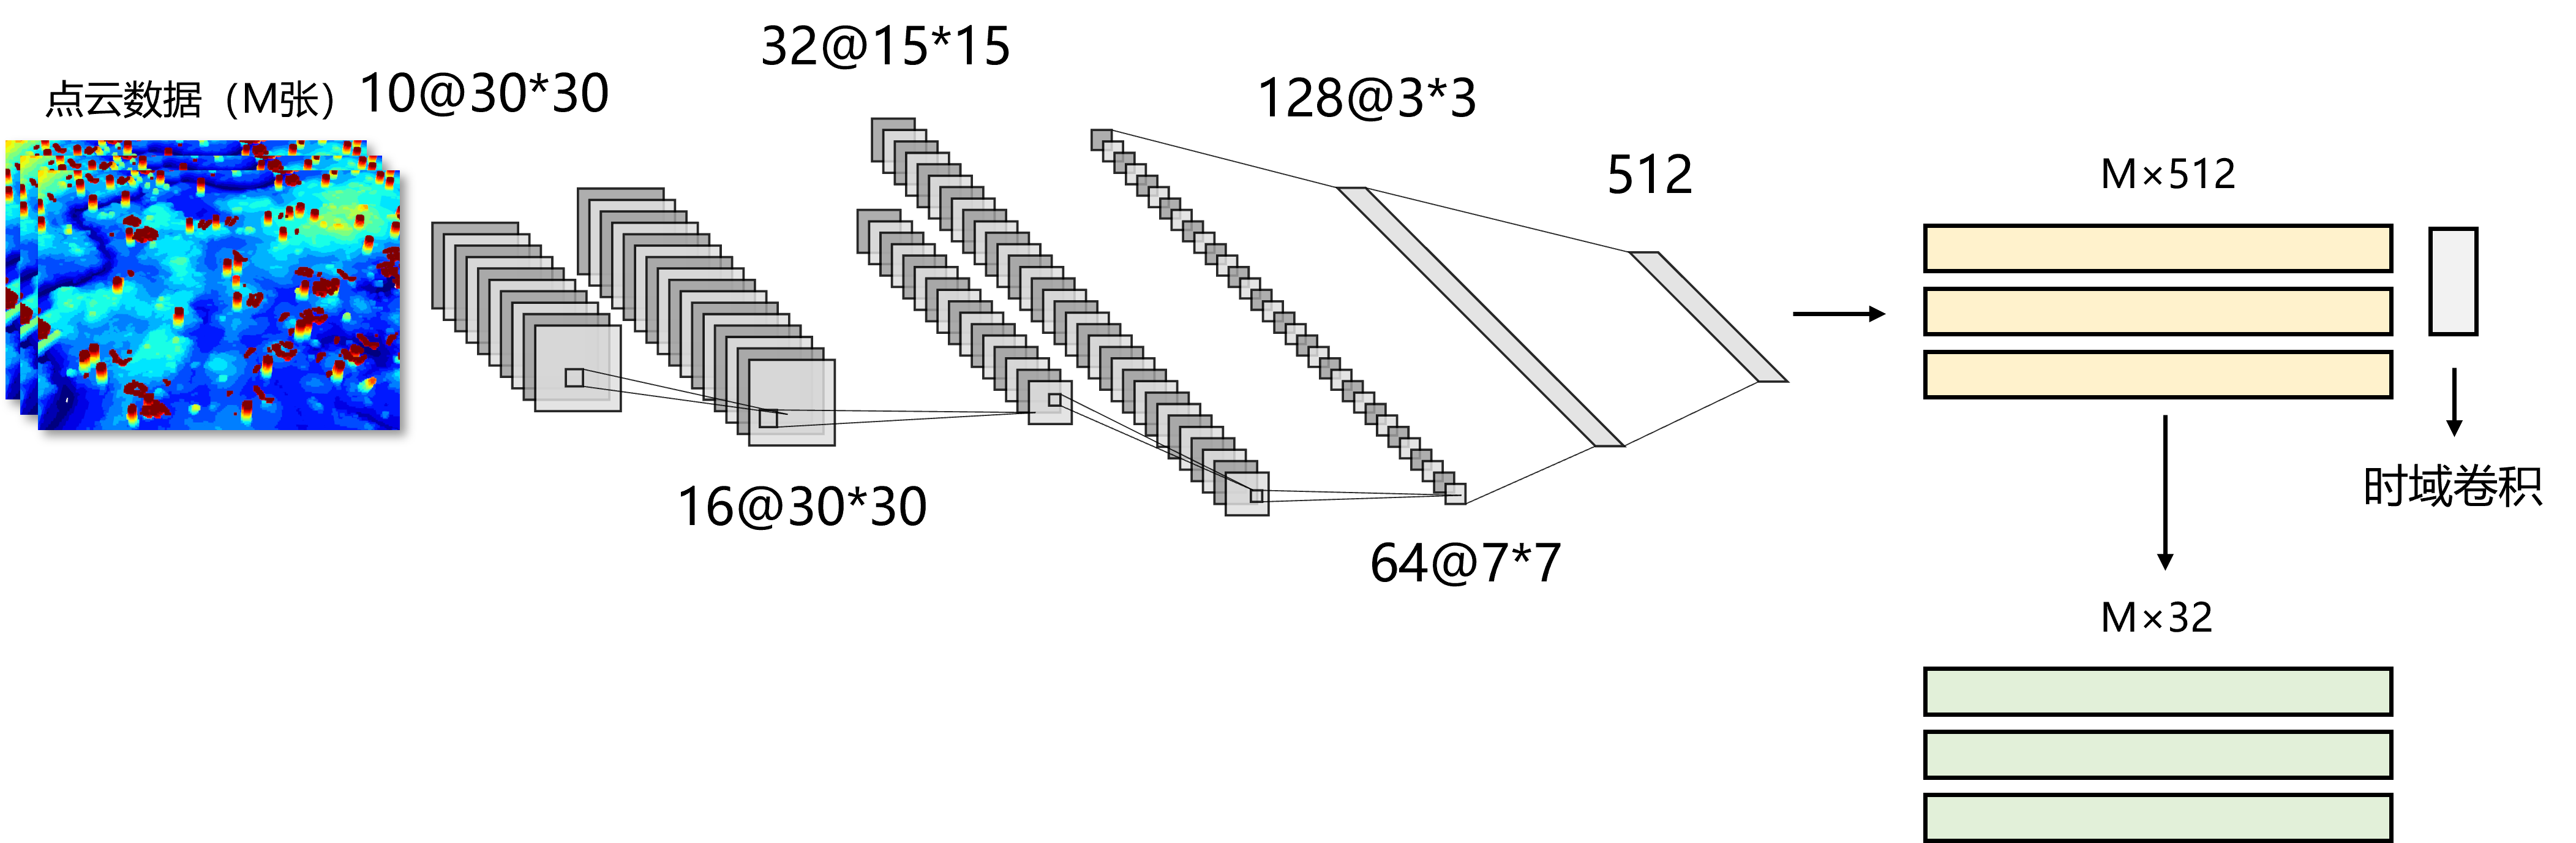
\includegraphics[width = 1\textwidth]{pcd_encoder.png}
  \caption{点云编码器结构图}
  \label{fig_pcd_encoder}
\end{figure}

\subsubsection{点云输入的强化学习训练}
在获得点云编码器后,就可以使用使用点云编码器连接输入,用\ref{PPO_alg}节提到的PPO算法训练规划器。具体训练流程如图\ref{fig_step2}所示。训练中使用的奖励函数$\mathcal{R}$将在\ref{reward_design}节中详细介绍。在训练中为了进一步提高训练效率,还设计了以下两个技术细节:
\begin{enumerate}
  \item 编码器固定。强化学习的基本原理决定了其需要通过试错来改进策略。在训练最开始阶段,策略是几乎随机的。若编码器也被同时训练,可能会降低预训练编码器的性能。故在训练开始时先固定编码器参数,仅改变规划器使其能够在固定的编码器下学到较好的策略。当规划器训练到一定程度(具体表现为平均回合长度达到6s,即策略学会了基本的飞行)后,再开始以较低的更新率一同训练编码器,以微调其编码能力。
  \item 域随机化(Domain randomization)。在训练时将障碍物密度、起始位置、飞行参考速度等任务参数在一定比例范围内随机化,增加训练数据的多样性,提高模型的泛化能力。
\end{enumerate}

\subsubsection{编码器对齐}

使用点云作为输入是为了加速训练,而实际应用和部署的阶段仍需要深度相机拍摄的深度图作为输入。因此训练的最后一步就是以调整过后的点云编码器为监督,训练深度图编码器。我们采集了约$3\times 10^5$组数据,每组数据都有一张深度图和一块点云组成,采用有监督学习的方法。具体训练流程如图\ref{fig_step3}。训练过程中使用均方误差(Mean Square Error, MSE)损失函数。两种编码器虽输入不同,但编码完成后在相同环境的情况下其编码产生的嵌入(Embedding)应是相似的,因此可以接在相同的规划器前完成相同的任务。

在使用如上所述的三段式训练方法后,在线强化学习阶段的数据采集效率提升了1$\sim$2个数量级,从约60FPS提升至约3000FPS。而第一三阶段的监督训练在NVIDIA GeForce RTX 4090 GPU环境下所需时间仅以在10分钟量级,相比在线强化学习训练的时间几乎可以忽略不计。三段式训练方法大大提升了训练效率。在第\ref{result}章的结果分析中可以看到使用编码器对齐技术的自主导航算法在性能上的损失也非常小。

\subsection{奖励设计}
\label{reward_design}
\begin{figure}
  \centering
  \includegraphics[width = 1\textwidth]{reward.png}
  \caption{计算奖励函数示意图}
  \label{fig_reward}
\end{figure}
在强化学习中,奖励函数$\mathcal{R}$的设计是十分重要的。奖励函数的设计直接影响到强化学习的训练效率和最终的性能。为了更好地评判智能体完成导航任务的情况,在训练和部署的过程中引入参考轨迹(Reference trajectory),这是一条连接任务起始点和终点的直线轨迹,每$0.04m$取一个点。在训练中,取轨迹长为$40m$的一条直线轨迹,记作$\psi$,其中$\psi(k)$表示轨迹上第$k$个点的空间位置。如图\ref{fig_reward}所示,设飞行器在$t$时刻的位置为$p(t)$,速度为 $v(t)$,角速度为$\omega(t)$,总推力(由策略采集的动作给出)为$ct(t)$。定义
\[\begin{aligned}
  k(t) &= {\arg\min}_k {||p(t)-\psi(k)||}\\
  a &= ||p(t)-\psi(k(t))||
\end{aligned}\]
分别表示参考轨迹上距飞行器最近点的编号和飞行器距最近点的距离。再定义
\[
  s(p(t)) = \sum_{i=1}^{k(t)} ||\psi(i)-\psi(i-1)||
\]
表示参考轨迹上距飞行器最近点在参考轨迹上与初始点的距离。这样奖励函数中与导航任务进度相关的几项便可以定义:
\[\begin{aligned}
  r_p &= k(t)-k(t-1)\\
  r_a &= a(t-1)-a(t)\\
\end{aligned}\]
在定义与飞行状态相关的几项:
\[\begin{aligned}
  r_\omega &= -||\omega(t)||^2\\
  r_v &= -||v(t)-v_\text{ref}||^2\\
  r_e & = -||ct(t)||^2\\
\end{aligned}\]
而$R_T$是一项离散的奖励,当飞机碰撞障碍时为$-10$,到达目标点时为$+10$,其余情况为$0$。

结合自主导航的任务设定,本研究的奖励函数设计为:
\[
  R(t) = k_Tr_T + k_\omega r_\omega + k_v r_v+ k_p r_p + k_s s(p(t))+ k_e r_e + k_a r_a
\]
其中$k_i$表示第$i$项的系数,用于平衡各项奖励在总奖励中的占比。

奖励函数中$r_p,\ s(p(t))$两项鼓励智能体向目标点前进,$r_a$项惩罚飞行器离参考轨迹过远,$r_\omega,\ r_v,\ r_e$三项惩罚飞行器采取过于激进的飞行状态,$R_T$惩罚飞行器碰撞障碍物并鼓励飞行器到达目标点。该奖励函数综合考虑了重要事件带来的稀疏奖励(Sparse reward)和飞行过程中的连续奖励(Dense reward),能够有效地指导智能体完成导航任务。

\section{本章小结}

本章介绍了本研究的核心创新点:一种自主导航算法框架和配套的三段式训练方法。算法框架由编码器和规划器组成。三段式训练方法从解决训练瓶颈的角度出发,使用点云替代深度图做输入加速训练,并使用编码器固定等方式加快算法收敛,最后使用编码器对齐的方式得到部署和应用所需的深度图编码器从而完成整个算法的训练。通过这样的设计,算法训练效率提升了一个数量级。本章还介绍了训练过程中的其他细节,例如输入输出的选择、奖励函数的设计等。算法部分调试的参数和训练结果将在第\ref{result}章展开。
% \section{数学符号}

% 中文论文的数学符号默认遵循 GB/T 3102.11—1993《物理科学和技术中使用的数学符号》
% \footnote{原 GB 3102.11—1993,自 2017 年 3 月 23 日起,该标准转为推荐性标准。}。
% 该标准参照采纳 ISO 31-11:1992 \footnote{目前已更新为 ISO 80000-2:2019。},
% 但是与 \TeX{} 默认的美国数学学会(AMS)的符号习惯有所区别。
% 具体地来说主要有以下差异:
% \begin{enumerate}
%   \item 大写希腊字母默认为斜体,如
%     \begin{equation*}
%       \Gamma \Delta \Theta \Lambda \Xi \Pi \Sigma \Upsilon \Phi \Psi \Omega.
%     \end{equation*}
%     注意有限增量符号 $\increment$ 固定使用正体,模板提供了 \cs{increment} 命令。
%   \item 小于等于号和大于等于号使用倾斜的字形 $\le$、$\ge$。
%   \item 积分号使用正体,比如 $\int$、$\oint$。
%   \item
%     偏微分符号 $\partial$ 使用正体。
%   \item
%     省略号 \cs{dots} 按照中文的习惯固定居中,比如
%     \begin{equation*}
%       1, 2, \dots, n \quad 1 + 2 + \dots + n.
%     \end{equation*}
%   \item
%     实部 $\Re$ 和虚部 $\Im$ 的字体使用罗马体。
% \end{enumerate}

% 以上数学符号样式的差异可以在模板中统一设置。
% 另外国标还有一些与 AMS 不同的符号使用习惯,需要用户在写作时进行处理:
% \begin{enumerate}
%   \item 数学常数和特殊函数名用正体,如
%     \begin{equation*}
%       \uppi = 3.14\dots; \quad
%       \symup{i}^2 = -1; \quad
%       \symup{e} = \lim_{n \to \infty} \left( 1 + \frac{1}{n} \right)^n.
%     \end{equation*}
%   \item 微分号使用正体,比如 $\dif y / \dif x$。
%   \item 向量、矩阵和张量用粗斜体(\cs{symbf}),如 $\symbf{x}$、$\symbf{\Sigma}$、$\symbfsf{T}$。
%   \item 自然对数用 $\ln x$ 不用 $\log x$。
% \end{enumerate}


% 英文论文的数学符号使用 \TeX{} 默认的样式。
% 如果有必要,也可以通过设置 \verb|math-style| 选择数学符号样式。

% 关于量和单位推荐使用
% \href{http://mirrors.ctan.org/macros/latex/contrib/siunitx/siunitx.pdf}{\pkg{siunitx}}
% 宏包,
% 可以方便地处理希腊字母以及数字与单位之间的空白,
% 比如:
% \SI{6.4e6}{m},
% \SI{9}{\micro\meter},
% \si{kg.m.s^{-1}},
% \SIrange{10}{20}{\degreeCelsius}。



% \section{数学公式}

% 数学公式可以使用 \env{equation} 和 \env{equation*} 环境。
% 注意数学公式的引用应前后带括号,通常使用 \cs{eqref} 命令,比如式\eqref{eq:example}。
% \begin{equation}
%   \frac{1}{2 \uppi \symup{i}} \int_\gamma f = \sum_{k=1}^m n(\gamma; a_k) \mathscr{R}(f; a_k).
%   \label{eq:example}
% \end{equation}

% 多行公式尽可能在“=”处对齐,推荐使用 \env{align} 环境。
% \begin{align}
%   a & = b + c + d + e \\
%     & = f + g
% \end{align}



% \section{数学定理}

% 定理环境的格式可以使用 \pkg{amsthm} 或者 \pkg{ntheorem} 宏包配置。
% 用户在导言区载入这两者之一后,模板会自动配置 \env{thoerem}、\env{proof} 等环境。

% \begin{theorem}[Lindeberg--Lévy 中心极限定理]
%   设随机变量 $X_1, X_2, \dots, X_n$ 独立同分布, 且具有期望 $\mu$ 和有限的方差 $\sigma^2 \ne 0$,
%   记 $\bar{X}_n = \frac{1}{n} \sum_{i+1}^n X_i$,则
%   \begin{equation}
%     \lim_{n \to \infty} P \left(\frac{\sqrt{n} \left( \bar{X}_n - \mu \right)}{\sigma} \le z \right) = \Phi(z),
%   \end{equation}
%   其中 $\Phi(z)$ 是标准正态分布的分布函数。
% \end{theorem}
% \begin{proof}
%   Trivial.
% \end{proof}

% 同时模板还提供了 \env{assumption}、\env{definition}、\env{proposition}、
% \env{lemma}、\env{theorem}、\env{axiom}、\env{corollary}、\env{exercise}、
% \env{example}、\env{remar}、\env{problem}、\env{conjecture} 这些相关的环境。

% !TeX root = ../thuthesis-example.tex

\chapter{部署平台设计}
一个完备的飞行部署平台应具备性能稳定、接口完善、易用性高等优点。目前市面上尚没有一种满足本研究算法部署需求的平台。本研究从硬件选型、装配再到部署系统的开发,设计了整个部署平台。本部署平台的开发参考了相关工作的开源硬件平台\cite{zhou2020ego}和控制系统\cite{Faessler18ral}。

\section{硬件平台搭建}

截止本报告撰写,为本研究设计的自主无人机已经迭代三个版本。如图\ref{}所示。这三个版本无人机的功能改进如表\ref{}所示。最新版本自主无人机的基本参数如表\ref{}所示。
% 详细的硬件平台选型及各部件基本参数如附录\ref{}所示。

\section{部署系统}
本研究基于ROS开发了一套运行于机载计算机上的部署系统。部署系统的主要功能是收集传感器的输入、提供算法接口、为飞行器保证基本的飞行能力、以及与底层执行器(在本研究中是飞行控制器)通信。本研究开发的部署系统结构如图\ref{}所示,每个方框表示一个ROS节点。

\subsection{系统输入}
系统的输入与表\ref{tab_input}所示一致。其中VIO的算法被嵌入式地集成到定位相机模块中,定位相机会直接输出飞行器的位置、姿态和速度信息。深度图的信息直接来源于深度相机模块。

为增强定位系统的稳定性,本研究同样使用飞行控制器携带的IMU读取位姿信息。部署系统与飞行控制器通过Mavros桥(\ref{mavros_bridge}节)通信,读取IMU信息并使用增强卡尔曼滤波\cite{kalman1960contributions}\cite{kalman1960new}\cite{kalman1961new}(extended Kalman filter, EKF)融合定位相机与IMU的信息,得到更可靠的飞行器位姿信息。

\subsection{算法接口}
本部署框架于AUtopilot节点内集成了模型预测控制器\cite{Falanga2018}(Model predict control, MPC)和比例-积分-微分控制器(Proportion-integration-differentiation, PID)控制器。通过封装,两个控制器均可以接受五种不同的命令输入,并将他们转换为统一的输出。输出有两种模式可供选择。输入和输出命令的具体介绍如表\ref{tab_autopilot_input}和表\ref{tab_autopilot_output}所示。

\begin{table}[!ht]
    \centering
    \begin{tabular}{ccl}
    \hline
        \textbf{输入名称} & \textbf{输入内容} & \textbf{输入描述} \\ \hline
        pos\_command & $(x,\ y,\ z)$ & 指定空间中一点,按照直线飞行至该位置。 \\ 
        velo\_command & $(v_x,\ v_y,\ v_z,\ \omega_{z})$ & 指定线速度和$z$向角速度,按照该速度飞行。 \\ 
        \multirow{3}*{ref\_command} & 一个轨迹点(Trajectory Point): & 指定轨迹点,使飞行器的状态与轨迹点尽 \\ 
        & $(x,\ y,\ z,\ \text{roll, pitch, yaw})$ & 可能接近。通常轨迹点与当前状态差别不 \\
        & 及其$1\sim3$阶时间导数 & 大,连续发送轨迹点以实现光滑控制。 \\
        traj\_command & 一串轨迹点 & 从初始位置连续飞行全部轨迹点 \\ 
        control\_command & 控制器输出的指令格式 & 控制器不工作 \\ \hline
    \end{tabular}
    \caption{集成控制器可选输入}
    \label{tab_autopilot_input}
\end{table}

\begin{table}[!ht]
    \centering
    \begin{tabular}{ccl}
    \hline
        \textbf{输出模式} & \textbf{输出内容} & \textbf{输入描述} \\ \hline
        attitude & $(\text{thrust},\ \text{roll, pitch, yaw})$ & 飞行器的总推力和目标姿态 \\ 
        bodyrates & $(\text{thrust},\ \omega_x,\ \omega_y,\ \omega_z)$ & 即CTBR命令 \\ \hline
    \end{tabular}
    \caption{集成控制器可选输出}
    \label{tab_autopilot_output}
\end{table}

\subsection{状态切换}
\subsection{Mavros桥}
\label{mavros_bridge}
\subsection{部署系统的基本性能}

%此处应包含部署系统的基础能力测试

% 模板支持 BibTeX 和 BibLaTeX 两种方式处理参考文献。
% 下文主要介绍 BibTeX 配合 \pkg{natbib} 宏包的主要使用方法。


% \section{顺序编码制}

% 在顺序编码制下,默认的 \cs{cite} 命令同 \cs{citep} 一样,序号置于方括号中,
% 引文页码会放在括号外。
% 统一处引用的连续序号会自动用短横线连接。

% \thusetup{
%   cite-style = super,
% }
% \noindent
% \begin{tabular}{l@{\quad$\Rightarrow$\quad}l}
%   \verb|\cite{zhangkun1994}|               & \cite{zhangkun1994}               \\
%   \verb|\citet{zhangkun1994}|              & \citet{zhangkun1994}              \\
%   \verb|\citep{zhangkun1994}|              & \citep{zhangkun1994}              \\
%   \verb|\cite[42]{zhangkun1994}|           & \cite[42]{zhangkun1994}           \\
%   \verb|\cite{zhangkun1994,zhukezhen1973}| & \cite{zhangkun1994,zhukezhen1973} \\
% \end{tabular}


% 也可以取消上标格式,将数字序号作为文字的一部分。
% 建议全文统一使用相同的格式。

% \thusetup{
%   cite-style = inline,
% }
% \noindent
% \begin{tabular}{l@{\quad$\Rightarrow$\quad}l}
%   \verb|\cite{zhangkun1994}|               & \cite{zhangkun1994}               \\
%   \verb|\citet{zhangkun1994}|              & \citet{zhangkun1994}              \\
%   \verb|\citep{zhangkun1994}|              & \citep{zhangkun1994}              \\
%   \verb|\cite[42]{zhangkun1994}|           & \cite[42]{zhangkun1994}           \\
%   \verb|\cite{zhangkun1994,zhukezhen1973}| & \cite{zhangkun1994,zhukezhen1973} \\
% \end{tabular}



% \section{著者-出版年制}

% 著者-出版年制下的 \cs{cite} 跟 \cs{citet} 一样。

% \thusetup{
%   cite-style = author-year,
% }
% \noindent
% \begin{tabular}{@{}l@{$\Rightarrow$}l@{}}
%   \verb|\cite{zhangkun1994}|                & \cite{zhangkun1994}                \\
%   \verb|\citet{zhangkun1994}|               & \citet{zhangkun1994}               \\
%   \verb|\citep{zhangkun1994}|               & \citep{zhangkun1994}               \\
%   \verb|\cite[42]{zhangkun1994}|            & \cite[42]{zhangkun1994}            \\
%   \verb|\citep{zhangkun1994,zhukezhen1973}| & \citep{zhangkun1994,zhukezhen1973} \\
% \end{tabular}

% \vskip 2ex
% \thusetup{
%   cite-style = super,
% }
% 注意,引文参考文献的每条都要在正文中标注
% \cite{zhangkun1994,zhukezhen1973,dupont1974bone,zhengkaiqing1987,%
%   jiangxizhou1980,jianduju1994,merkt1995rotational,mellinger1996laser,%
%   bixon1996dynamics,mahui1995,carlson1981two,taylor1983scanning,%
%   taylor1981study,shimizu1983laser,atkinson1982experimental,%
%   kusch1975perturbations,guangxi1993,huosini1989guwu,wangfuzhi1865songlun,%
%   zhaoyaodong1998xinshidai,biaozhunhua2002tushu,chubanzhuanye2004,%
%   who1970factors,peebles2001probability,baishunong1998zhiwu,%
%   weinstein1974pathogenic,hanjiren1985lun,dizhi1936dizhi,%
%   tushuguan1957tushuguanxue,aaas1883science,fugang2000fengsha,%
%   xiaoyu2001chubanye,oclc2000about,scitor2000project%
% }。



% 其他部分
\backmatter

\listoffigures           % 插图清单
\listoftables            % 附表清单


% 参考文献
\bibliography{ref/refs}  % 参考文献使用 BibTeX 编译
% \printbibliography       % 参考文献使用 BibLaTeX 编译

% 附录
% 本科生需要将附录放到声明之后,个人简历之前

% % !TeX root = ../thuthesis-example.tex

\begin{survey}
\label{cha:survey}

\title{Title of the Survey}
\maketitle


\tableofcontents


本科生的外文资料调研阅读报告。


\section{Figures and Tables}

\subsection{Figures}

An example figure in appendix (Figure~\ref{fig:appendix-survey-figure}).

\begin{figure}
  \centering
  
\includegraphics[width=0.6\linewidth]{example-image-a.pdf}
  \caption{Example figure in appendix}
  \label{fig:appendix-survey-figure}
\end{figure}


\subsection{Tables}

An example table in appendix (Table~\ref{tab:appendix-survey-table}).

\begin{table}
  \centering
  \caption{Example table in appendix}
  \begin{tabular}{ll}
    \toprule
    File name       & Description                                         \\
    \midrule
    thuthesis.dtx   & The source file including documentaion and comments \\
    thuthesis.cls   & The template file                                   \\
    thuthesis-*.bst & BibTeX styles                                       \\
    thuthesis-*.bbx & BibLaTeX styles for bibliographies                  \\
    thuthesis-*.cbx & BibLaTeX styles for citations                       \\
    \bottomrule
  \end{tabular}
  \label{tab:appendix-survey-table}
\end{table}


\section{Equations}

An example equation in appendix (Equation~\eqref{eq:appendix-survey-equation}).
\begin{equation}
  \frac{1}{2 \uppi \symup{i}} \int_\gamma f = \sum_{k=1}^m n(\gamma; a_k) \mathscr{R}(f; a_k)
  \label{eq:appendix-survey-equation}
\end{equation}


\section{Citations}

Example citations in appendix.
\cite{abrahams99tex}
\cite{salomon1995advanced}
\cite{abrahams99tex,salomon1995advanced}


\bibliographystyle{unsrtnat}
\bibliography{ref/appendix}

\end{survey}
       % 本科生:外文资料的调研阅读报告
% % !TeX root = ../thuthesis-example.tex

\begin{translation}
\label{cha:translation}

\title{书面翻译题目}
\maketitle

\tableofcontents


本科生的外文资料书面翻译。


\section{图表示例}

\subsection{图}

附录中的图片示例(图~\ref{fig:appendix-translation-figure})。

\begin{figure}
  \centering
  
\includegraphics[width=0.6\linewidth]{example-image-a.pdf}
  \caption{附录中的图片示例}
  \label{fig:appendix-translation-figure}
\end{figure}


\subsection{表格}

附录中的表格示例(表~\ref{tab:appendix-translation-table})。

\begin{table}
  \centering
  \caption{附录中的表格示例}
  \begin{tabular}{ll}
    \toprule
    文件名          & 描述                         \\
    \midrule
    thuthesis.dtx   & 模板的源文件,包括文档和注释 \\
    thuthesis.cls   & 模板文件                     \\
    thuthesis-*.bst & BibTeX 参考文献表样式文件    \\
    thuthesis-*.bbx & BibLaTeX 参考文献表样式文件  \\
    thuthesis-*.cbx & BibLaTeX 引用样式文件        \\
    \bottomrule
  \end{tabular}
  \label{tab:appendix-translation-table}
\end{table}


\section{数学公式}

附录中的数学公式示例(公式\eqref{eq:appendix-translation-equation})。
\begin{equation}
  \frac{1}{2 \uppi \symup{i}} \int_\gamma f = \sum_{k=1}^m n(\gamma; a_k) \mathscr{R}(f; a_k)
  \label{eq:appendix-translation-equation}
\end{equation}


\section{文献引用}

文献引用示例\cite{abrahams99tex}。


\appendix

\section{附录}

附录的内容。


% 书面翻译的参考文献
\bibliographystyle{unsrtnat}
\bibliography{ref/appendix}

% 书面翻译对应的原文索引
\begin{translation-index}
  \nocite{salomon1995advanced}
  \bibliographystyle{unsrtnat}
  \bibliography{ref/appendix}
\end{translation-index}

\end{translation}
  % 本科生:外文资料的书面翻译
% % !TeX root = ../thuthesis-example.tex

\chapter{补充内容}

附录是与论文内容密切相关、但编入正文又影响整篇论文编排的条理和逻辑性的资料,例如某些重要的数据表格、计算程序、统计表等,是论文主体的补充内容,可根据需要设置。

附录中的图、表、数学表达式、参考文献等另行编序号,与正文分开,一律用阿拉伯数字编码,
但在数码前冠以附录的序号,例如“图~\ref{fig:appendix-figure}”,
“表~\ref{tab:appendix-table}”,“式\eqref{eq:appendix-equation}”等。


\section{插图}

% 附录中的插图示例(图~\ref{fig:appendix-figure})。

\begin{figure}
  \centering
  
\includegraphics[width=0.6\linewidth]{example-image-a.pdf}
  \caption{附录中的图片示例}
  \label{fig:appendix-figure}
\end{figure}


\section{表格}

% 附录中的表格示例(表~\ref{tab:appendix-table})。

\begin{table}
  \centering
  \caption{附录中的表格示例}
  \begin{tabular}{ll}
    \toprule
    文件名          & 描述                         \\
    \midrule
    thuthesis.dtx   & 模板的源文件,包括文档和注释 \\
    thuthesis.cls   & 模板文件                     \\
    thuthesis-*.bst & BibTeX 参考文献表样式文件    \\
    thuthesis-*.bbx & BibLaTeX 参考文献表样式文件  \\
    thuthesis-*.cbx & BibLaTeX 引用样式文件        \\
    \bottomrule
  \end{tabular}
  \label{tab:appendix-table}
\end{table}


\section{数学表达式}

% 附录中的数学表达式示例(式\eqref{eq:appendix-equation})。
\begin{equation}
  \frac{1}{2 \uppi \symup{i}} \int_\gamma f = \sum_{k=1}^m n(\gamma; a_k) \mathscr{R}(f; a_k)
  \label{eq:appendix-equation}
\end{equation}


\section{参考文献}

附录中的参考文献示例(\cite{carlson1981two} 和 \cite{carlson1981two,taylor1983scanning,taylor1981study})。

%\printbibliography


% 致谢
% !TeX root = ../thuthesis-example.tex

\begin{acknowledgements}
  衷心感谢导师×××教授和物理系××副教授对本人的精心指导。他们的言传身教将使我终生受益。

  在美国麻省理工学院化学系进行九个月的合作研究期间,承蒙 Robert Field 教授热心指导与帮助,不胜感激。

  感谢×××××实验室主任×××教授,以及实验室全体老师和同窗们学的热情帮助和支持!

  本课题承蒙国家自然科学基金资助,特此致谢。
\end{acknowledgements}


% 声明
\statement
% 将签字扫描后的声明文件 scan-statement.pdf 替换原始页面
% \statement[file=scan-statement.pdf]
% 本科生编译生成的声明页默认不加页脚,插入扫描版时再补上;
% 研究生编译生成时有页眉页脚,插入扫描版时不再重复。
% 也可以手动控制是否加页眉页脚
% \statement[page-style=empty]
% \statement[file=scan-statement.pdf, page-style=plain]

\appendix


% 个人简历、在学期间完成的相关学术成果
% 本科生可以附个人简历,也可以不附个人简历
%% !TeX root = ../thuthesis-example.tex

\begin{resume}

  \section*{个人简历}

  197× 年 ×× 月 ×× 日出生于四川××县。

  1992 年 9 月考入××大学化学系××化学专业,1996 年 7 月本科毕业并获得理学学士学位。

  1996 年 9 月免试进入清华大学化学系攻读××化学博士至今。


  \section*{在学期间完成的相关学术成果}

  \subsection*{学术论文}

  \begin{achievements}
    \item Yang Y, Ren T L, Zhang L T, et al. Miniature microphone with silicon-based ferroelectric thin films[J]. Integrated Ferroelectrics, 2003, 52:229-235.
    \item 杨轶, 张宁欣, 任天令, 等. 硅基铁电微声学器件中薄膜残余应力的研究[J]. 中国机械工程, 2005, 16(14):1289-1291.
    \item 杨轶, 张宁欣, 任天令, 等. 集成铁电器件中的关键工艺研究[J]. 仪器仪表学报, 2003, 24(S4):192-193.
    \item Yang Y, Ren T L, Zhu Y P, et al. PMUTs for handwriting recognition. In press[J]. (已被Integrated Ferroelectrics录用)
  \end{achievements}


  \subsection*{专利}

  \begin{achievements}
    \item 任天令, 杨轶, 朱一平, 等. 硅基铁电微声学传感器畴极化区域控制和电极连接的方法: 中国, CN1602118A[P]. 2005-03-30.
    \item Ren T L, Yang Y, Zhu Y P, et al. Piezoelectric micro acoustic sensor based on ferroelectric materials: USA, No.11/215, 102[P]. (美国发明专利申请号.)
  \end{achievements}

\end{resume}


% 指导教师/指导小组评语
% 本科生不需要
%% !TeX root = ../thuthesis-example.tex

\begin{comments}
% \begin{comments}[name = {指导小组评语}]
% \begin{comments}[name = {Comments from Thesis Supervisor}]
% \begin{comments}[name = {Comments from Thesis Supervision Committee}]

  论文提出了……

\end{comments}


% 答辩委员会决议书
% 本科生不需要
%% !TeX root = ../thuthesis-example.tex

\begin{resolution}

  论文提出了……

  论文取得的主要创新性成果包括:

  1. ……

  2. ……

  3. ……

  论文工作表明作者在×××××具有×××××知识,具有××××能力,论文××××,答辩××××。

  答辩委员会表决,(×票/一致)同意通过论文答辩,并建议授予×××(姓名)×××(门类)学博士/硕士学位。

\end{resolution}


% 本科生的综合论文训练记录表(扫描版)
% \record{file=scan-record.pdf}

\end{document}
